\documentclass[twoside]{book}

% Packages required by doxygen
\usepackage{fixltx2e}
\usepackage{calc}
\usepackage{doxygen}
\usepackage[export]{adjustbox} % also loads graphicx
\usepackage{graphicx}
\usepackage[utf8]{inputenc}
\usepackage{makeidx}
\usepackage{multicol}
\usepackage{multirow}
\PassOptionsToPackage{warn}{textcomp}
\usepackage{textcomp}
\usepackage[nointegrals]{wasysym}
\usepackage[table]{xcolor}

% Font selection
\usepackage[T1]{fontenc}
\usepackage[scaled=.90]{helvet}
\usepackage{courier}
\usepackage{amssymb}
\usepackage{sectsty}
\renewcommand{\familydefault}{\sfdefault}
\allsectionsfont{%
  \fontseries{bc}\selectfont%
  \color{darkgray}%
}
\renewcommand{\DoxyLabelFont}{%
  \fontseries{bc}\selectfont%
  \color{darkgray}%
}
\newcommand{\+}{\discretionary{\mbox{\scriptsize$\hookleftarrow$}}{}{}}

% Page & text layout
\usepackage{geometry}
\geometry{%
  a4paper,%
  top=2.5cm,%
  bottom=2.5cm,%
  left=2.5cm,%
  right=2.5cm%
}
\tolerance=750
\hfuzz=15pt
\hbadness=750
\setlength{\emergencystretch}{15pt}
\setlength{\parindent}{0cm}
\setlength{\parskip}{3ex plus 2ex minus 2ex}
\makeatletter
\renewcommand{\paragraph}{%
  \@startsection{paragraph}{4}{0ex}{-1.0ex}{1.0ex}{%
    \normalfont\normalsize\bfseries\SS@parafont%
  }%
}
\renewcommand{\subparagraph}{%
  \@startsection{subparagraph}{5}{0ex}{-1.0ex}{1.0ex}{%
    \normalfont\normalsize\bfseries\SS@subparafont%
  }%
}
\makeatother

% Headers & footers
\usepackage{fancyhdr}
\pagestyle{fancyplain}
\fancyhead[LE]{\fancyplain{}{\bfseries\thepage}}
\fancyhead[CE]{\fancyplain{}{}}
\fancyhead[RE]{\fancyplain{}{\bfseries\leftmark}}
\fancyhead[LO]{\fancyplain{}{\bfseries\rightmark}}
\fancyhead[CO]{\fancyplain{}{}}
\fancyhead[RO]{\fancyplain{}{\bfseries\thepage}}
\fancyfoot[LE]{\fancyplain{}{}}
\fancyfoot[CE]{\fancyplain{}{}}
\fancyfoot[RE]{\fancyplain{}{\bfseries\scriptsize Generated by Doxygen }}
\fancyfoot[LO]{\fancyplain{}{\bfseries\scriptsize Generated by Doxygen }}
\fancyfoot[CO]{\fancyplain{}{}}
\fancyfoot[RO]{\fancyplain{}{}}
\renewcommand{\footrulewidth}{0.4pt}
\renewcommand{\chaptermark}[1]{%
  \markboth{#1}{}%
}
\renewcommand{\sectionmark}[1]{%
  \markright{\thesection\ #1}%
}

% Indices & bibliography
\usepackage{natbib}
\usepackage[titles]{tocloft}
\setcounter{tocdepth}{3}
\setcounter{secnumdepth}{5}
\makeindex

% Hyperlinks (required, but should be loaded last)
\usepackage{ifpdf}
\ifpdf
  \usepackage[pdftex,pagebackref=true]{hyperref}
\else
  \usepackage[ps2pdf,pagebackref=true]{hyperref}
\fi
\hypersetup{%
  colorlinks=true,%
  linkcolor=blue,%
  citecolor=blue,%
  unicode%
}

% Custom commands
\newcommand{\clearemptydoublepage}{%
  \newpage{\pagestyle{empty}\cleardoublepage}%
}

\usepackage{caption}
\captionsetup{labelsep=space,justification=centering,font={bf},singlelinecheck=off,skip=4pt,position=top}

%===== C O N T E N T S =====

\begin{document}

% Titlepage & ToC
\hypersetup{pageanchor=false,
             bookmarksnumbered=true,
             pdfencoding=unicode
            }
\pagenumbering{alph}
\begin{titlepage}
\vspace*{7cm}
\begin{center}%
{\Large R\+OS Navigation from Scratch }\\
\vspace*{1cm}
{\large Generated by Doxygen 1.8.13}\\
\end{center}
\end{titlepage}
\clearemptydoublepage
\pagenumbering{roman}
\tableofcontents
\clearemptydoublepage
\pagenumbering{arabic}
\hypersetup{pageanchor=true}

%--- Begin generated contents ---
\chapter{Navigation in R\+OS from Scratch}
\label{index}\hypertarget{index}{}\subsection*{Description}

This repository contains files that that implements odometry and E\+KF S\+L\+AM for a differential drive robot, as well as various supporting libraries and testing nodes. Currently, there is no path planning implementation. The currently repository also contains files to run everything on the Turtle\+Bot3 Burger.

\subsection*{Packages}

Here is a high level description of each package, more details for the nodes and libraries can be found in the A\+PI.


\begin{DoxyItemize}
\item {\ttfamily rigid2d}\+: This package contains nodes and libraries that support all of the odometry based functions.
\item {\ttfamily nuslam}\+: This package contains nodes and libraries that support all of the S\+L\+AM based functions.
\item {\ttfamily tsim}\+: This package contains nodes to test various features of the rigid2d package using the built in turtle sim in R\+OS.
\item {\ttfamily nuturtle\+\_\+robot}\+: This package contains nodes to interface the odometry and S\+L\+AM packages to the Turtle\+Bot3.
\item {\ttfamily nuturtle\+\_\+gazebo}\+: This package contains a gazebo plugin to run a Turtle\+Bot3 in simulation using the existing files.
\item {\ttfamily nuturtle\+\_\+description}\+: This package contains all files relevant to the robots visualizations.
\end{DoxyItemize}

Select libraries and functions also have accompanying test files usings {\ttfamily gtest} and {\ttfamily rostest}.

\subsection*{How to use this repo\+:}

Most likely entirety of this repo will not be plug and play since a lot all of the real world implementations are configured for our lab\textquotesingle{}s specific turtlebots with stripped down firmware targeted at this project. But everything should work out of the box if you use the simulation options instead of the real world options.

\subsubsection*{1) Get all of the necessary files.}

Use the nuturtle.\+rosinstall file to clone this repo as well a peripheral one that contains some custom messages

\subsubsection*{2) Launch something!}

\paragraph*{The main launch files\+:}


\begin{DoxyItemize}
\item {\ttfamily nuslam/slam.\+launch}\+: This file will run the full S\+L\+AM implementation along side a comparison to only odometry. It currently uses the keyboard teleop control to send velocity commands to the turtlebot. Check out demo videos here.
\end{DoxyItemize}

\subparagraph*{Parameters\+:}


\begin{DoxyItemize}
\item robot\+: Use a value of -\/1 to launch everything based on a gazebo simulation. Using a number $>$ 0 will launch everything using a robot in the real world.
\item debug\+: Use 1 to feed the S\+L\+AM node groundtruth data to do the pose estimation. Use 0 to feed S\+L\+AM the slam node data from the actual laser scanner.
\end{DoxyItemize}

{\ttfamily nuturtle\+\_\+robot/follow\+\_\+waypoints.\+launch}\+: This file will run a waypoint following script that uses only odometry to estimate the robot pose as it follows a list of waypoints and compares the pose to the \textquotesingle{}perfect\textquotesingle{} robot (nodes in the {\ttfamily fake} namespace). Once launched, call the {\ttfamily /start} service to actually start sending velocity commands. Once the path has been completed, call {\ttfamily /start} again to complete another loop. Currently only proportional control is used to follow the waypoints. Check out a demo video \href{https://www.youtube.com/watch?v=V_Ljk7B5whE}{\tt here}.

To use this file with the simulated robot, just launch {\ttfamily nuturtle\+\_\+gazebo/gazebo\+\_\+waypoints.\+launch}. No need to pass any arguments.

\subparagraph*{Parameters\+:}


\begin{DoxyItemize}
\item robot\+: Using a number $>$ 0 will launch everything using a robot in the real world. See the lower section for how to set this up. 0 will launch everything only on the local machine and should only be used for testing or running locally on the turtlebot.
\item with\+\_\+rviz\+: Use True to also launch rviz.
\end{DoxyItemize}

\paragraph*{The other launch files\+:}

{\ttfamily nuslam}\+:
\begin{DoxyItemize}
\item {\ttfamily landmarks.\+launch}\+: test laser scan landmark detection and visualization
\item {\ttfamily analysis\+\_\+landmarks.\+launch}\+: test gazebo landmark data conversion and visualization {\ttfamily nuturtle\+\_\+description}\+:
\item {\ttfamily view\+\_\+diff\+\_\+drive.\+launch}\+: view the robot urdf file in rviz
\end{DoxyItemize}

{\ttfamily nuturtle\+\_\+gazebo}\+:
\begin{DoxyItemize}
\item {\ttfamily diff\+\_\+drive\+\_\+gazebo.\+launch}\+: test file for plugin development
\end{DoxyItemize}

{\ttfamily nuturtle\+\_\+robot}\+:
\begin{DoxyItemize}
\item {\ttfamily basic\+\_\+remote.\+launch}\+: used to configure the interface between the real robot and your computer for running remotely.
\item {\ttfamily teleop\+\_\+turtle.\+launch}\+: used to launch odometry with turtlebot3\textquotesingle{}s keyboard teleop node.
\item {\ttfamily test\+\_\+movement.\+launch}\+: used to test the interface between the robot sensor data and the odometry calculations.
\end{DoxyItemize}

{\ttfamily tsim}\+:
\begin{DoxyItemize}
\item {\ttfamily trect.\+launch}\+: uses turtle sim to test the rigid2d and diff drive libraries with feed-\/forward control.
\item {\ttfamily turtle\+\_\+odom.\+launch}\+: uses turtle sim to test the odometer and encoder simulation node.
\item {\ttfamily turtle\+\_\+pent.\+launch}\+: uses turtle sim to test waypoiont following library.
\end{DoxyItemize}

\subsection*{Under the hood\+:}

All of the odometry calculations are built on the conversions from the desired body velocity to individual wheel velocity commands that actually are sent to the robot. The derivation for this can be found \href{nuturtle_robot/doc/Kinematics.pdf}{\tt here} in the rigid2d package.

This S\+L\+AM implementation is using an E\+KF to perform the pose estimation for the robot and each landmark. \href{https://nu-msr.github.io/navigation_site/slam.pdf}{\tt Here} is a detailed resource for practically implementing the E\+KF.

This implementation has the constraint that all of the landmarks it expects to see are cylindrical pillars of a uniform radius. The landmarks are identified using laser scan data reported by the simulation/real robot. First the laser scan data is divided into clusters based on the range values reported by the scanner. If a cluster has more than 3 data points it is then processed using a circle fitting algorithm based on this \href{https://nu-msr.github.io/navigation_site/circle_fit.html}{\tt practical guide} to identify the center and estimated radius. For more information on the circle fitting see this \href{https://projecteuclid.org/euclid.ejs/1251119958}{\tt paper} and related \href{https://people.cas.uab.edu/~mosya/cl/CPPcircle.html}{\tt website}. After fitting the circle any fit with a radius greater than the threshold parameter is discarded. Initially, a \href{http://miarn.sourceforge.net/pdf/a1738b.pdf}{\tt classification algorithm} based on this paper was also implemented, but it yielded worse results than screening by radius in this application.

 In order to associate incoming data with the current estimation of the landmark states, Euclidean distance was used. If the the distance between a data point and an estimated landmark is under a minimum threshold it is considered a match to an existing landmark. If the distance between a data point and all estimated landmarks is greater than a maximum threshold it is considered a new landmark. An alternative option for associating data points is using the Mahalanobis distance. While this method is more complex, it has the advantage of taking into account the covarience of the estimated pose. See this \href{https://nu-msr.github.io/navigation_site/data_assoc.html}{\tt resource} for how to implement this type of data association. 
\chapter{nuturtle\+\_\+description Description}
\label{md_nuturtle_description_README}
\Hypertarget{md_nuturtle_description_README}
This package contains files to create robot descriptions suitable for simulation. It contains various urdf/xacro files and basic debugging, testing, and visualization code for the robots used in the other packages.

\section*{How to run\+:}

Copy the following into a console window\+:  
\begin{DoxyCode}
roslaunch nuturtle\_description view\_diff\_drive.launch
\end{DoxyCode}


\section*{File Tree\+:}


\begin{DoxyCode}
├── config
│   ├── diff\_params.yaml - contains parameters to define a generic diff drive robot
│   └── view\_urdf.rviz - rviz config file
├── launch
│   └── view\_diff\_drive.launch - main launch file to view diff drive robot
└── urdf
    └── diff\_drive.urdf.xacro - xacro file that generates a diff drive robot
\end{DoxyCode}
 
\chapter{tsim Description}
\label{md_tsim_README}
\Hypertarget{md_tsim_README}
This package is used to control the turtlesim simulation.

\section*{How to run\+:}

{\ttfamily roslaunch tsim trect.\+launch} -\/ It uses feedforward control to drive the turtle in a rectangle based on the parameters set in the yaml file. It also calculates and plots the positional error.

{\ttfamily roslaunch tsim turtle\+\_\+pent.\+launch} -\/ Drives the turtle in a pentagon using the Waypoints and Diff\+Drive classes from rigid2d.

{\ttfamily roslaunch tsim trutle\+\_\+odom.\+launch} -\/ Uses {\ttfamily fake\+\_\+diff\+\_\+encoders} and {\ttfamily odometer} nodes to control a diff drive robot in rviz to mimic the turtle. (This launch file includes {\ttfamily turtle\+\_\+pent.\+launch})


\begin{DoxyCode}
├── config
│   └── turtle\_rect\_params.yaml - parameters the determine the turtle trajectory
├── launch
│   ├── trect.launch
│   ├── turtle\_odom.launch
│   └── turtle\_pent.launch
├── msg
│   └── PoseError.msg - custom message to publish positional error values
└── src
    ├── turtle\_rect.cpp - main source file for turtle\_rect node
    └── turtle\_way.cpp - main source file for turtle\_way node
\end{DoxyCode}


\section*{Results}

\subsection*{For {\ttfamily turtle\+\_\+rect.\+launch}}

\href{https://youtu.be/aji3aDB8LBI}{\tt Video Link}

  

\subsection*{For {\ttfamily turtle\+\_\+pent.\+launch}}



\subsection*{For {\ttfamily turtle\+\_\+odom.\+launch}}

\href{https://youtu.be/058QKyPgfmI}{\tt Video link} 
\chapter{Hierarchical Index}
\section{Class Hierarchy}
This inheritance list is sorted roughly, but not completely, alphabetically\+:\begin{DoxyCompactList}
\item \contentsline{section}{rigid2d\+:\+:Diff\+Drive}{\pageref{classrigid2d_1_1DiffDrive}}{}
\item Model\+Plugin\begin{DoxyCompactList}
\item \contentsline{section}{gazebo\+:\+:Turtle\+Drive\+Plugin}{\pageref{classgazebo_1_1TurtleDrivePlugin}}{}
\end{DoxyCompactList}
\item \contentsline{section}{rigid2d\+:\+:Pose2D}{\pageref{structrigid2d_1_1Pose2D}}{}
\item \contentsline{section}{Pose\+Vals}{\pageref{structPoseVals}}{}
\item \contentsline{section}{ekf\+\_\+slam\+:\+:Slam}{\pageref{classekf__slam_1_1Slam}}{}
\item \contentsline{section}{rigid2d\+:\+:Transform2D}{\pageref{classrigid2d_1_1Transform2D}}{}
\item \contentsline{section}{rigid2d\+:\+:Twist2D}{\pageref{structrigid2d_1_1Twist2D}}{}
\item \contentsline{section}{rigid2d\+:\+:Vector2D}{\pageref{structrigid2d_1_1Vector2D}}{}
\item \contentsline{section}{rigid2d\+:\+:Waypoints}{\pageref{classrigid2d_1_1Waypoints}}{}
\item \contentsline{section}{rigid2d\+:\+:Wheel\+Velocities}{\pageref{structrigid2d_1_1WheelVelocities}}{}
\end{DoxyCompactList}

\chapter{Class Index}
\section{Class List}
Here are the classes, structs, unions and interfaces with brief descriptions\+:\begin{DoxyCompactList}
\item\contentsline{section}{\hyperlink{classrigid2d_1_1DiffDrive}{rigid2d\+::\+Diff\+Drive} }{\pageref{classrigid2d_1_1DiffDrive}}{}
\item\contentsline{section}{\hyperlink{structrigid2d_1_1Pose2D}{rigid2d\+::\+Pose2D} \\*A 2-\/\+Dimensional Pose }{\pageref{structrigid2d_1_1Pose2D}}{}
\item\contentsline{section}{\hyperlink{structPoseVals}{Pose\+Vals} \\*A struct to hold related positional values }{\pageref{structPoseVals}}{}
\item\contentsline{section}{\hyperlink{classekf__slam_1_1Slam}{ekf\+\_\+slam\+::\+Slam} }{\pageref{classekf__slam_1_1Slam}}{}
\item\contentsline{section}{\hyperlink{classrigid2d_1_1Transform2D}{rigid2d\+::\+Transform2D} \\*Rigid body transformation in 2 dimensions }{\pageref{classrigid2d_1_1Transform2D}}{}
\item\contentsline{section}{\hyperlink{classgazebo_1_1TurtleDrivePlugin}{gazebo\+::\+Turtle\+Drive\+Plugin} }{\pageref{classgazebo_1_1TurtleDrivePlugin}}{}
\item\contentsline{section}{\hyperlink{structrigid2d_1_1Twist2D}{rigid2d\+::\+Twist2D} \\*A 2-\/\+Dimensional Twist }{\pageref{structrigid2d_1_1Twist2D}}{}
\item\contentsline{section}{\hyperlink{structrigid2d_1_1Vector2D}{rigid2d\+::\+Vector2D} \\*A 2-\/\+Dimensional Vector }{\pageref{structrigid2d_1_1Vector2D}}{}
\item\contentsline{section}{\hyperlink{classrigid2d_1_1Waypoints}{rigid2d\+::\+Waypoints} }{\pageref{classrigid2d_1_1Waypoints}}{}
\item\contentsline{section}{\hyperlink{structrigid2d_1_1WheelVelocities}{rigid2d\+::\+Wheel\+Velocities} \\*Wheel velocities for a diff drive robot }{\pageref{structrigid2d_1_1WheelVelocities}}{}
\end{DoxyCompactList}

\chapter{File Index}
\section{File List}
Here is a list of all documented files with brief descriptions\+:\begin{DoxyCompactList}
\item\contentsline{section}{nuslam/include/nuslam/\hyperlink{cylinder__detect_8hpp}{cylinder\+\_\+detect.\+hpp} \\*Function to fit circles }{\pageref{cylinder__detect_8hpp}}{}
\item\contentsline{section}{nuslam/include/nuslam/\hyperlink{ekf__slam_8hpp}{ekf\+\_\+slam.\+hpp} \\*Library to contain S\+L\+AM class and supporting functions }{\pageref{ekf__slam_8hpp}}{}
\item\contentsline{section}{nuslam/src/\hyperlink{analysis_8cpp}{analysis.\+cpp} \\*This node takes the information from gazebo and publishes it for debuggin S\+L\+AM node }{\pageref{analysis_8cpp}}{}
\item\contentsline{section}{nuslam/src/\hyperlink{draw__map_8cpp}{draw\+\_\+map.\+cpp} \\*This node takes a list of centers and radii to draw the coresponding map }{\pageref{draw__map_8cpp}}{}
\item\contentsline{section}{nuslam/src/\hyperlink{landmarks_8cpp}{landmarks.\+cpp} \\*This node clusters laser scan data points and fits each cluster to a circular landmark }{\pageref{landmarks_8cpp}}{}
\item\contentsline{section}{nuslam/src/\hyperlink{slam_8cpp}{slam.\+cpp} \\*This node publishes an estimate of the robot state using E\+KF S\+L\+AM }{\pageref{slam_8cpp}}{}
\item\contentsline{section}{nuslam/test/\hyperlink{test__landmarks_8cpp}{test\+\_\+landmarks.\+cpp} \\*This node tests the landmark node circle fitting functions }{\pageref{test__landmarks_8cpp}}{}
\item\contentsline{section}{nuturtle\+\_\+robot/src/\hyperlink{real__waypoints_8cpp}{real\+\_\+waypoints.\+cpp} \\*This node publishes a twist to drive the turtlebot along a path of waypoints }{\pageref{real__waypoints_8cpp}}{}
\item\contentsline{section}{nuturtle\+\_\+robot/src/\hyperlink{rotation_8cpp}{rotation.\+cpp} \\*This node interfaces between a main computer and the raspberri pi on the turtlebot }{\pageref{rotation_8cpp}}{}
\item\contentsline{section}{nuturtle\+\_\+robot/src/\hyperlink{turtle__interface_8cpp}{turtle\+\_\+interface.\+cpp} \\*This node interfaces between a main computer and the raspberri pi on the turtlebot }{\pageref{turtle__interface_8cpp}}{}
\item\contentsline{section}{nuturtle\+\_\+robot/src/test/\hyperlink{test__turtle__interface_8cpp}{test\+\_\+turtle\+\_\+interface.\+cpp} \\*This node tests the turtle interface node }{\pageref{test__turtle__interface_8cpp}}{}
\item\contentsline{section}{rigid2d/include/rigid2d/\hyperlink{diff__drive_8hpp}{diff\+\_\+drive.\+hpp} \\*Library for tracking the state of a diff drive robot }{\pageref{diff__drive_8hpp}}{}
\item\contentsline{section}{rigid2d/include/rigid2d/\hyperlink{rigid2d_8hpp}{rigid2d.\+hpp} \\*Library for two-\/dimensional rigid body transformations }{\pageref{rigid2d_8hpp}}{}
\item\contentsline{section}{rigid2d/include/rigid2d/\hyperlink{waypoints_8hpp}{waypoints.\+hpp} \\*Library for calculating the velocities to move between waypoints }{\pageref{waypoints_8hpp}}{}
\item\contentsline{section}{rigid2d/src/\hyperlink{fake__diff__encoders_8cpp}{fake\+\_\+diff\+\_\+encoders.\+cpp} \\*This file contains the source code for the turtle\+\_\+rect node. It pulls in parameters set from the yaml file and uses feed forward control to drive the turtle in a rectangle. It also calculates the positional error over time }{\pageref{fake__diff__encoders_8cpp}}{}
\item\contentsline{section}{rigid2d/src/\hyperlink{odometer_8cpp}{odometer.\+cpp} \\*This node publishes the Odometry messages per R\+OS standard format }{\pageref{odometer_8cpp}}{}
\item\contentsline{section}{rigid2d/src/\hyperlink{rigid2d__node_8cpp}{rigid2d\+\_\+node.\+cpp} \\*Manipulates 2D Transforms, Vectors, and Twists to test the ridig2d files }{\pageref{rigid2d__node_8cpp}}{}
\item\contentsline{section}{rigid2d/src/rigid2d/\hyperlink{diff__drive_8cpp}{diff\+\_\+drive.\+cpp} \\*Source file for Diff Dirve Robot library }{\pageref{diff__drive_8cpp}}{}
\item\contentsline{section}{rigid2d/src/rigid2d/\hyperlink{rigid2d_8cpp}{rigid2d.\+cpp} \\*Source file for rigid2D 2D Transformation library }{\pageref{rigid2d_8cpp}}{}
\item\contentsline{section}{rigid2d/src/rigid2d/\hyperlink{waypoints_8cpp}{waypoints.\+cpp} \\*Library for calculating the velocities to move between waypoints }{\pageref{waypoints_8cpp}}{}
\item\contentsline{section}{tsim/src/\hyperlink{turtle__rect_8cpp}{turtle\+\_\+rect.\+cpp} \\*This file contains the source code for the turtle\+\_\+rect node. It pulls in parameters set from the yaml file and uses feed forward control to drive the turtle in a rectangle. It also calculates the positional error over time }{\pageref{turtle__rect_8cpp}}{}
\item\contentsline{section}{tsim/src/\hyperlink{turtle__way_8cpp}{turtle\+\_\+way.\+cpp} \\*This file contains the source code for the turtle\+\_\+way node. It reads in a list of waypoints and sends commands to turtlesim to follow that path }{\pageref{turtle__way_8cpp}}{}
\end{DoxyCompactList}

\chapter{Class Documentation}
\hypertarget{classrigid2d_1_1DiffDrive}{}\section{rigid2d\+:\+:Diff\+Drive Class Reference}
\label{classrigid2d_1_1DiffDrive}\index{rigid2d\+::\+Diff\+Drive@{rigid2d\+::\+Diff\+Drive}}
\subsection*{Public Member Functions}
\begin{DoxyCompactItemize}
\item 
\mbox{\Hypertarget{classrigid2d_1_1DiffDrive_a2d646290b7a03d391a59e8a296fea30d}\label{classrigid2d_1_1DiffDrive_a2d646290b7a03d391a59e8a296fea30d}} 
\hyperlink{classrigid2d_1_1DiffDrive_a2d646290b7a03d391a59e8a296fea30d}{Diff\+Drive} ()
\begin{DoxyCompactList}\small\item\em the default constructor creates a robot at (0,0,0), with a default wheel base and wheel radius \end{DoxyCompactList}\item 
\hyperlink{classrigid2d_1_1DiffDrive_a5af54c5b7f4bacebb75a287031e792b4}{Diff\+Drive} (\hyperlink{structrigid2d_1_1Pose2D}{Pose2D} \hyperlink{classrigid2d_1_1DiffDrive_a3af583df8981ddfb338bba07b7297ff2}{pose}, double wheel\+\_\+base, double wheel\+\_\+radius)
\begin{DoxyCompactList}\small\item\em create a \hyperlink{classrigid2d_1_1DiffDrive}{Diff\+Drive} model by specifying the pose, and geometry \end{DoxyCompactList}\item 
\hyperlink{structrigid2d_1_1WheelVelocities}{Wheel\+Velocities} \hyperlink{classrigid2d_1_1DiffDrive_a636194ac11bb3851059989ae118bbf1d}{twist\+To\+Wheels} (\hyperlink{structrigid2d_1_1Twist2D}{Twist2D} twist)
\begin{DoxyCompactList}\small\item\em determine the wheel velocities required to make the robot move with the desired linear and angular velocities. See doc directory for derivation. \end{DoxyCompactList}\item 
\hyperlink{structrigid2d_1_1Twist2D}{Twist2D} \hyperlink{classrigid2d_1_1DiffDrive_a34f3a4df7a14565563a6b56d8eef2b9b}{wheels\+To\+Twist} (\hyperlink{structrigid2d_1_1WheelVelocities}{Wheel\+Velocities} vel) const
\begin{DoxyCompactList}\small\item\em determine the body twist of the robot from its wheel velocities. See doc directory for derivation. \end{DoxyCompactList}\item 
\hyperlink{structrigid2d_1_1WheelVelocities}{Wheel\+Velocities} \hyperlink{classrigid2d_1_1DiffDrive_aa037844753d585eca7023bfd935e084b}{update\+Odometry} (double left, double right)
\begin{DoxyCompactList}\small\item\em Update the robot\textquotesingle{}s odometry based on the current encoder readings. \end{DoxyCompactList}\item 
void \hyperlink{classrigid2d_1_1DiffDrive_a09e8b9b8fe6539b75bb08f1b71242b7c}{feedforward} (\hyperlink{structrigid2d_1_1Twist2D}{Twist2D} cmd)
\begin{DoxyCompactList}\small\item\em update the odometry of the diff drive robot, assuming that it follows the given body twist for one time unit \end{DoxyCompactList}\item 
void \hyperlink{classrigid2d_1_1DiffDrive_adc465e5cf9027ffb207a3775800d2033}{set\+Radius} (double radius)
\begin{DoxyCompactList}\small\item\em Sets the wheel radius. \end{DoxyCompactList}\item 
void \hyperlink{classrigid2d_1_1DiffDrive_aed9b82741312243d9ea1f705afc372dc}{set\+Base} (double b)
\begin{DoxyCompactList}\small\item\em Sets the wheel base. \end{DoxyCompactList}\item 
\hyperlink{structrigid2d_1_1Pose2D}{Pose2D} \hyperlink{classrigid2d_1_1DiffDrive_a3af583df8981ddfb338bba07b7297ff2}{pose} () const
\begin{DoxyCompactList}\small\item\em get the current pose of the robot \end{DoxyCompactList}\item 
\hyperlink{structrigid2d_1_1WheelVelocities}{Wheel\+Velocities} \hyperlink{classrigid2d_1_1DiffDrive_add7b4cb6d5e4edaffdcefbfa930a2f43}{get\+Encoders} () const
\begin{DoxyCompactList}\small\item\em get the current absolute encoder position \end{DoxyCompactList}\item 
\hyperlink{structrigid2d_1_1WheelVelocities}{Wheel\+Velocities} \hyperlink{classrigid2d_1_1DiffDrive_a4153bdc614be0535b88d5e43461df7dc}{wheel\+Velocities} () const
\begin{DoxyCompactList}\small\item\em get the wheel speeds, based on the last encoder update \end{DoxyCompactList}\item 
void \hyperlink{classrigid2d_1_1DiffDrive_afffa18508c27b368767182dba1a7d367}{reset} (\hyperlink{structrigid2d_1_1Pose2D}{Pose2D} ps)
\begin{DoxyCompactList}\small\item\em reset the robot to the given position/orientation \end{DoxyCompactList}\end{DoxyCompactItemize}


\subsection{Constructor \& Destructor Documentation}
\mbox{\Hypertarget{classrigid2d_1_1DiffDrive_a5af54c5b7f4bacebb75a287031e792b4}\label{classrigid2d_1_1DiffDrive_a5af54c5b7f4bacebb75a287031e792b4}} 
\index{rigid2d\+::\+Diff\+Drive@{rigid2d\+::\+Diff\+Drive}!Diff\+Drive@{Diff\+Drive}}
\index{Diff\+Drive@{Diff\+Drive}!rigid2d\+::\+Diff\+Drive@{rigid2d\+::\+Diff\+Drive}}
\subsubsection{\texorpdfstring{Diff\+Drive()}{DiffDrive()}}
{\footnotesize\ttfamily rigid2d\+::\+Diff\+Drive\+::\+Diff\+Drive (\begin{DoxyParamCaption}\item[{\hyperlink{structrigid2d_1_1Pose2D}{Pose2D}}]{pose,  }\item[{double}]{wheel\+\_\+base,  }\item[{double}]{wheel\+\_\+radius }\end{DoxyParamCaption})}



create a \hyperlink{classrigid2d_1_1DiffDrive}{Diff\+Drive} model by specifying the pose, and geometry 


\begin{DoxyParams}{Parameters}
{\em pose} & -\/ the current position of the robot \\
\hline
{\em wheel\+\_\+base} & -\/ the distance between the wheel centers \\
\hline
{\em wheel\+\_\+radius} & -\/ the raidus of the wheels \\
\hline
\end{DoxyParams}


\subsection{Member Function Documentation}
\mbox{\Hypertarget{classrigid2d_1_1DiffDrive_a09e8b9b8fe6539b75bb08f1b71242b7c}\label{classrigid2d_1_1DiffDrive_a09e8b9b8fe6539b75bb08f1b71242b7c}} 
\index{rigid2d\+::\+Diff\+Drive@{rigid2d\+::\+Diff\+Drive}!feedforward@{feedforward}}
\index{feedforward@{feedforward}!rigid2d\+::\+Diff\+Drive@{rigid2d\+::\+Diff\+Drive}}
\subsubsection{\texorpdfstring{feedforward()}{feedforward()}}
{\footnotesize\ttfamily void rigid2d\+::\+Diff\+Drive\+::feedforward (\begin{DoxyParamCaption}\item[{\hyperlink{structrigid2d_1_1Twist2D}{Twist2D}}]{cmd }\end{DoxyParamCaption})}



update the odometry of the diff drive robot, assuming that it follows the given body twist for one time unit 


\begin{DoxyParams}{Parameters}
{\em cmd} & -\/ the twist command to send to the robot \\
\hline
\end{DoxyParams}
\mbox{\Hypertarget{classrigid2d_1_1DiffDrive_add7b4cb6d5e4edaffdcefbfa930a2f43}\label{classrigid2d_1_1DiffDrive_add7b4cb6d5e4edaffdcefbfa930a2f43}} 
\index{rigid2d\+::\+Diff\+Drive@{rigid2d\+::\+Diff\+Drive}!get\+Encoders@{get\+Encoders}}
\index{get\+Encoders@{get\+Encoders}!rigid2d\+::\+Diff\+Drive@{rigid2d\+::\+Diff\+Drive}}
\subsubsection{\texorpdfstring{get\+Encoders()}{getEncoders()}}
{\footnotesize\ttfamily \hyperlink{structrigid2d_1_1WheelVelocities}{Wheel\+Velocities} rigid2d\+::\+Diff\+Drive\+::get\+Encoders (\begin{DoxyParamCaption}{ }\end{DoxyParamCaption}) const}



get the current absolute encoder position 

\begin{DoxyReturn}{Returns}
the encoder position 
\end{DoxyReturn}
\mbox{\Hypertarget{classrigid2d_1_1DiffDrive_a3af583df8981ddfb338bba07b7297ff2}\label{classrigid2d_1_1DiffDrive_a3af583df8981ddfb338bba07b7297ff2}} 
\index{rigid2d\+::\+Diff\+Drive@{rigid2d\+::\+Diff\+Drive}!pose@{pose}}
\index{pose@{pose}!rigid2d\+::\+Diff\+Drive@{rigid2d\+::\+Diff\+Drive}}
\subsubsection{\texorpdfstring{pose()}{pose()}}
{\footnotesize\ttfamily \hyperlink{structrigid2d_1_1Pose2D}{Pose2D} rigid2d\+::\+Diff\+Drive\+::pose (\begin{DoxyParamCaption}{ }\end{DoxyParamCaption}) const}



get the current pose of the robot 

\begin{DoxyReturn}{Returns}
the current pose of the robot 
\end{DoxyReturn}
\mbox{\Hypertarget{classrigid2d_1_1DiffDrive_afffa18508c27b368767182dba1a7d367}\label{classrigid2d_1_1DiffDrive_afffa18508c27b368767182dba1a7d367}} 
\index{rigid2d\+::\+Diff\+Drive@{rigid2d\+::\+Diff\+Drive}!reset@{reset}}
\index{reset@{reset}!rigid2d\+::\+Diff\+Drive@{rigid2d\+::\+Diff\+Drive}}
\subsubsection{\texorpdfstring{reset()}{reset()}}
{\footnotesize\ttfamily void rigid2d\+::\+Diff\+Drive\+::reset (\begin{DoxyParamCaption}\item[{\hyperlink{structrigid2d_1_1Pose2D}{Pose2D}}]{ps }\end{DoxyParamCaption})}



reset the robot to the given position/orientation 


\begin{DoxyParams}{Parameters}
{\em ps} & -\/ the desired position/orientation to place the robot \\
\hline
\end{DoxyParams}
\mbox{\Hypertarget{classrigid2d_1_1DiffDrive_aed9b82741312243d9ea1f705afc372dc}\label{classrigid2d_1_1DiffDrive_aed9b82741312243d9ea1f705afc372dc}} 
\index{rigid2d\+::\+Diff\+Drive@{rigid2d\+::\+Diff\+Drive}!set\+Base@{set\+Base}}
\index{set\+Base@{set\+Base}!rigid2d\+::\+Diff\+Drive@{rigid2d\+::\+Diff\+Drive}}
\subsubsection{\texorpdfstring{set\+Base()}{setBase()}}
{\footnotesize\ttfamily void rigid2d\+::\+Diff\+Drive\+::set\+Base (\begin{DoxyParamCaption}\item[{double}]{b }\end{DoxyParamCaption})}



Sets the wheel base. 


\begin{DoxyParams}{Parameters}
{\em b} & -\/ value to update the class parameter to \\
\hline
\end{DoxyParams}
\mbox{\Hypertarget{classrigid2d_1_1DiffDrive_adc465e5cf9027ffb207a3775800d2033}\label{classrigid2d_1_1DiffDrive_adc465e5cf9027ffb207a3775800d2033}} 
\index{rigid2d\+::\+Diff\+Drive@{rigid2d\+::\+Diff\+Drive}!set\+Radius@{set\+Radius}}
\index{set\+Radius@{set\+Radius}!rigid2d\+::\+Diff\+Drive@{rigid2d\+::\+Diff\+Drive}}
\subsubsection{\texorpdfstring{set\+Radius()}{setRadius()}}
{\footnotesize\ttfamily void rigid2d\+::\+Diff\+Drive\+::set\+Radius (\begin{DoxyParamCaption}\item[{double}]{radius }\end{DoxyParamCaption})}



Sets the wheel radius. 


\begin{DoxyParams}{Parameters}
{\em radius} & -\/ value to update the class parameter to \\
\hline
\end{DoxyParams}
\mbox{\Hypertarget{classrigid2d_1_1DiffDrive_a636194ac11bb3851059989ae118bbf1d}\label{classrigid2d_1_1DiffDrive_a636194ac11bb3851059989ae118bbf1d}} 
\index{rigid2d\+::\+Diff\+Drive@{rigid2d\+::\+Diff\+Drive}!twist\+To\+Wheels@{twist\+To\+Wheels}}
\index{twist\+To\+Wheels@{twist\+To\+Wheels}!rigid2d\+::\+Diff\+Drive@{rigid2d\+::\+Diff\+Drive}}
\subsubsection{\texorpdfstring{twist\+To\+Wheels()}{twistToWheels()}}
{\footnotesize\ttfamily \hyperlink{structrigid2d_1_1WheelVelocities}{Wheel\+Velocities} rigid2d\+::\+Diff\+Drive\+::twist\+To\+Wheels (\begin{DoxyParamCaption}\item[{\hyperlink{structrigid2d_1_1Twist2D}{Twist2D}}]{twist }\end{DoxyParamCaption})}



determine the wheel velocities required to make the robot move with the desired linear and angular velocities. See doc directory for derivation. 


\begin{DoxyParams}{Parameters}
{\em twist} & -\/ the desired twist in the body frame of the robot \\
\hline
\end{DoxyParams}
\begin{DoxyReturn}{Returns}
-\/ the wheel velocities to use 
\end{DoxyReturn}

\begin{DoxyExceptions}{Exceptions}
{\em std\+::exception} & when yb != 0 \\
\hline
\end{DoxyExceptions}
\mbox{\Hypertarget{classrigid2d_1_1DiffDrive_aa037844753d585eca7023bfd935e084b}\label{classrigid2d_1_1DiffDrive_aa037844753d585eca7023bfd935e084b}} 
\index{rigid2d\+::\+Diff\+Drive@{rigid2d\+::\+Diff\+Drive}!update\+Odometry@{update\+Odometry}}
\index{update\+Odometry@{update\+Odometry}!rigid2d\+::\+Diff\+Drive@{rigid2d\+::\+Diff\+Drive}}
\subsubsection{\texorpdfstring{update\+Odometry()}{updateOdometry()}}
{\footnotesize\ttfamily \hyperlink{structrigid2d_1_1WheelVelocities}{Wheel\+Velocities} rigid2d\+::\+Diff\+Drive\+::update\+Odometry (\begin{DoxyParamCaption}\item[{double}]{left,  }\item[{double}]{right }\end{DoxyParamCaption})}



Update the robot\textquotesingle{}s odometry based on the current encoder readings. 


\begin{DoxyParams}{Parameters}
{\em left} & -\/ the left encoder angle (in radians) \\
\hline
{\em right} & -\/ the right encoder angle (in radians) \\
\hline
\end{DoxyParams}
\begin{DoxyReturn}{Returns}
the velocities of each wheel, assuming that they have been constant since the last call to update\+Odometry 
\end{DoxyReturn}
\mbox{\Hypertarget{classrigid2d_1_1DiffDrive_a34f3a4df7a14565563a6b56d8eef2b9b}\label{classrigid2d_1_1DiffDrive_a34f3a4df7a14565563a6b56d8eef2b9b}} 
\index{rigid2d\+::\+Diff\+Drive@{rigid2d\+::\+Diff\+Drive}!wheels\+To\+Twist@{wheels\+To\+Twist}}
\index{wheels\+To\+Twist@{wheels\+To\+Twist}!rigid2d\+::\+Diff\+Drive@{rigid2d\+::\+Diff\+Drive}}
\subsubsection{\texorpdfstring{wheels\+To\+Twist()}{wheelsToTwist()}}
{\footnotesize\ttfamily \hyperlink{structrigid2d_1_1Twist2D}{Twist2D} rigid2d\+::\+Diff\+Drive\+::wheels\+To\+Twist (\begin{DoxyParamCaption}\item[{\hyperlink{structrigid2d_1_1WheelVelocities}{Wheel\+Velocities}}]{vel }\end{DoxyParamCaption}) const}



determine the body twist of the robot from its wheel velocities. See doc directory for derivation. 


\begin{DoxyParams}{Parameters}
{\em vel} & -\/ the velocities of the wheels, assumed to be held constant for one time unit \\
\hline
\end{DoxyParams}
\begin{DoxyReturn}{Returns}
twist in the original body frame of the robot 
\end{DoxyReturn}
\mbox{\Hypertarget{classrigid2d_1_1DiffDrive_a4153bdc614be0535b88d5e43461df7dc}\label{classrigid2d_1_1DiffDrive_a4153bdc614be0535b88d5e43461df7dc}} 
\index{rigid2d\+::\+Diff\+Drive@{rigid2d\+::\+Diff\+Drive}!wheel\+Velocities@{wheel\+Velocities}}
\index{wheel\+Velocities@{wheel\+Velocities}!rigid2d\+::\+Diff\+Drive@{rigid2d\+::\+Diff\+Drive}}
\subsubsection{\texorpdfstring{wheel\+Velocities()}{wheelVelocities()}}
{\footnotesize\ttfamily \hyperlink{structrigid2d_1_1WheelVelocities}{Wheel\+Velocities} rigid2d\+::\+Diff\+Drive\+::wheel\+Velocities (\begin{DoxyParamCaption}{ }\end{DoxyParamCaption}) const}



get the wheel speeds, based on the last encoder update 

\begin{DoxyReturn}{Returns}
the velocity of the wheels, which is equivalent to displacement because Delta\+\_\+T = 1 
\end{DoxyReturn}


The documentation for this class was generated from the following files\+:\begin{DoxyCompactItemize}
\item 
rigid2d/include/rigid2d/\hyperlink{diff__drive_8hpp}{diff\+\_\+drive.\+hpp}\item 
rigid2d/src/rigid2d/\hyperlink{diff__drive_8cpp}{diff\+\_\+drive.\+cpp}\end{DoxyCompactItemize}

\hypertarget{structrigid2d_1_1Pose2D}{}\section{rigid2d\+:\+:Pose2D Struct Reference}
\label{structrigid2d_1_1Pose2D}\index{rigid2d\+::\+Pose2D@{rigid2d\+::\+Pose2D}}


A 2-\/\+Dimensional Pose.  




{\ttfamily \#include $<$rigid2d.\+hpp$>$}

\subsection*{Public Member Functions}
\begin{DoxyCompactItemize}
\item 
\mbox{\Hypertarget{structrigid2d_1_1Pose2D_a88bf20c7ba06e18f9a8b01cef60e2c98}\label{structrigid2d_1_1Pose2D_a88bf20c7ba06e18f9a8b01cef60e2c98}} 
\hyperlink{structrigid2d_1_1Pose2D_a88bf20c7ba06e18f9a8b01cef60e2c98}{Pose2D} ()
\begin{DoxyCompactList}\small\item\em create an empty pose \end{DoxyCompactList}\item 
\hyperlink{structrigid2d_1_1Pose2D_aec3600c75f7341955ba7e8881cdd101a}{Pose2D} (double ang, double xpos, double ypos)
\begin{DoxyCompactList}\small\item\em create a pose \end{DoxyCompactList}\end{DoxyCompactItemize}
\subsection*{Public Attributes}
\begin{DoxyCompactItemize}
\item 
\mbox{\Hypertarget{structrigid2d_1_1Pose2D_aec39cadb59c95c2add01f01b07168a36}\label{structrigid2d_1_1Pose2D_aec39cadb59c95c2add01f01b07168a36}} 
double {\bfseries th} = 0.\+0
\item 
\mbox{\Hypertarget{structrigid2d_1_1Pose2D_a706d15249c213d0236481ff1bd13c42d}\label{structrigid2d_1_1Pose2D_a706d15249c213d0236481ff1bd13c42d}} 
double {\bfseries x} = 0.\+0
\item 
\mbox{\Hypertarget{structrigid2d_1_1Pose2D_a13f985853cc2b924ed87ed37e1857e7f}\label{structrigid2d_1_1Pose2D_a13f985853cc2b924ed87ed37e1857e7f}} 
double {\bfseries y} = 0.\+0
\end{DoxyCompactItemize}


\subsection{Detailed Description}
A 2-\/\+Dimensional Pose. 

\subsection{Constructor \& Destructor Documentation}
\mbox{\Hypertarget{structrigid2d_1_1Pose2D_aec3600c75f7341955ba7e8881cdd101a}\label{structrigid2d_1_1Pose2D_aec3600c75f7341955ba7e8881cdd101a}} 
\index{rigid2d\+::\+Pose2D@{rigid2d\+::\+Pose2D}!Pose2D@{Pose2D}}
\index{Pose2D@{Pose2D}!rigid2d\+::\+Pose2D@{rigid2d\+::\+Pose2D}}
\subsubsection{\texorpdfstring{Pose2\+D()}{Pose2D()}}
{\footnotesize\ttfamily rigid2d\+::\+Pose2\+D\+::\+Pose2D (\begin{DoxyParamCaption}\item[{double}]{ang,  }\item[{double}]{xpos,  }\item[{double}]{ypos }\end{DoxyParamCaption})}



create a pose 


\begin{DoxyParams}{Parameters}
{\em ang} & -\/ the angular heading \\
\hline
{\em xpos} & -\/ the x position \\
\hline
{\em ypos} & -\/ the y position \\
\hline
\end{DoxyParams}


The documentation for this struct was generated from the following files\+:\begin{DoxyCompactItemize}
\item 
rigid2d/include/rigid2d/\hyperlink{rigid2d_8hpp}{rigid2d.\+hpp}\item 
rigid2d/src/rigid2d/\hyperlink{rigid2d_8cpp}{rigid2d.\+cpp}\end{DoxyCompactItemize}

\hypertarget{structPoseVals}{}\section{Pose\+Vals Struct Reference}
\label{structPoseVals}\index{Pose\+Vals@{Pose\+Vals}}


A struct to hold related positional values.  


\subsection*{Public Attributes}
\begin{DoxyCompactItemize}
\item 
\mbox{\Hypertarget{structPoseVals_a142b98972fd33e398b5d2d39229a4fba}\label{structPoseVals_a142b98972fd33e398b5d2d39229a4fba}} 
double {\bfseries x}
\item 
\mbox{\Hypertarget{structPoseVals_a4f5f251edbab93cba37a4bd37b63d103}\label{structPoseVals_a4f5f251edbab93cba37a4bd37b63d103}} 
double {\bfseries y}
\item 
\mbox{\Hypertarget{structPoseVals_a70c84b784cbbb35c33d076e9493dcbd3}\label{structPoseVals_a70c84b784cbbb35c33d076e9493dcbd3}} 
double {\bfseries ang}
\end{DoxyCompactItemize}


\subsection{Detailed Description}
A struct to hold related positional values. 


\begin{DoxyParams}{Parameters}
{\em x} & -\/ xposition \\
\hline
{\em y} & -\/ yposition \\
\hline
{\em ang} & -\/ heading angle in radians \\
\hline
\end{DoxyParams}


The documentation for this struct was generated from the following file\+:\begin{DoxyCompactItemize}
\item 
tsim/src/\hyperlink{turtle__rect_8cpp}{turtle\+\_\+rect.\+cpp}\end{DoxyCompactItemize}

\hypertarget{classekf__slam_1_1Slam}{}\section{ekf\+\_\+slam\+:\+:Slam Class Reference}
\label{classekf__slam_1_1Slam}\index{ekf\+\_\+slam\+::\+Slam@{ekf\+\_\+slam\+::\+Slam}}
\subsection*{Public Member Functions}
\begin{DoxyCompactItemize}
\item 
\hyperlink{classekf__slam_1_1Slam_abc573b570700f3dfb0ff1e80c0263255}{Slam} (int num\+\_\+landmarks, Eigen\+::\+Matrix3d q\+\_\+var, Eigen\+::\+Matrix2d r\+\_\+var)
\begin{DoxyCompactList}\small\item\em Initialize an instance of E\+KF \hyperlink{classekf__slam_1_1Slam}{Slam}. Initializes the covarience matrix. \end{DoxyCompactList}\item 
void \hyperlink{classekf__slam_1_1Slam_ab26e0c13cbaaa3bce75be953f8c3b39d}{Motion\+Model\+Update} (\hyperlink{structrigid2d_1_1Twist2D}{rigid2d\+::\+Twist2D} tw)
\begin{DoxyCompactList}\small\item\em Predict the current state of the robot using the motion model. \end{DoxyCompactList}\item 
void \hyperlink{classekf__slam_1_1Slam_ae95105bbeeea067f5dc09e44e594dd3e}{Measurment\+Model\+Update} (nuslam\+::\+Turtle\+Map map\+\_\+data)
\begin{DoxyCompactList}\small\item\em Incorperate sensor information into the prediction from the motion model. \end{DoxyCompactList}\item 
std\+::vector$<$ double $>$ \hyperlink{classekf__slam_1_1Slam_a8c218402ba9d30177c6740d001430cac}{get\+Robot\+State} ()
\begin{DoxyCompactList}\small\item\em Extract the robot state. \end{DoxyCompactList}\item 
std\+::vector$<$ geometry\+\_\+msgs\+::\+Point $>$ \hyperlink{classekf__slam_1_1Slam_a66a7be45bb77f0c44717385908443832}{get\+Landmark\+States} ()
\begin{DoxyCompactList}\small\item\em Extract the landmark states. \end{DoxyCompactList}\end{DoxyCompactItemize}


\subsection{Constructor \& Destructor Documentation}
\mbox{\Hypertarget{classekf__slam_1_1Slam_abc573b570700f3dfb0ff1e80c0263255}\label{classekf__slam_1_1Slam_abc573b570700f3dfb0ff1e80c0263255}} 
\index{ekf\+\_\+slam\+::\+Slam@{ekf\+\_\+slam\+::\+Slam}!Slam@{Slam}}
\index{Slam@{Slam}!ekf\+\_\+slam\+::\+Slam@{ekf\+\_\+slam\+::\+Slam}}
\subsubsection{\texorpdfstring{Slam()}{Slam()}}
{\footnotesize\ttfamily ekf\+\_\+slam\+::\+Slam\+::\+Slam (\begin{DoxyParamCaption}\item[{int}]{num\+\_\+landmarks,  }\item[{Eigen\+::\+Matrix3d}]{q\+\_\+var,  }\item[{Eigen\+::\+Matrix2d}]{r\+\_\+var }\end{DoxyParamCaption})}



Initialize an instance of E\+KF \hyperlink{classekf__slam_1_1Slam}{Slam}. Initializes the covarience matrix. 


\begin{DoxyParams}{Parameters}
{\em num\+\_\+landmarks} & the number of landmarks in the map \\
\hline
{\em q\+\_\+var} & the process noise \\
\hline
{\em r\+\_\+var} & the sensor noise \\
\hline
\end{DoxyParams}


\subsection{Member Function Documentation}
\mbox{\Hypertarget{classekf__slam_1_1Slam_a66a7be45bb77f0c44717385908443832}\label{classekf__slam_1_1Slam_a66a7be45bb77f0c44717385908443832}} 
\index{ekf\+\_\+slam\+::\+Slam@{ekf\+\_\+slam\+::\+Slam}!get\+Landmark\+States@{get\+Landmark\+States}}
\index{get\+Landmark\+States@{get\+Landmark\+States}!ekf\+\_\+slam\+::\+Slam@{ekf\+\_\+slam\+::\+Slam}}
\subsubsection{\texorpdfstring{get\+Landmark\+States()}{getLandmarkStates()}}
{\footnotesize\ttfamily std\+::vector$<$ geometry\+\_\+msgs\+::\+Point $>$ ekf\+\_\+slam\+::\+Slam\+::get\+Landmark\+States (\begin{DoxyParamCaption}{ }\end{DoxyParamCaption})}



Extract the landmark states. 

\begin{DoxyReturn}{Returns}
a vector of the points 
\end{DoxyReturn}
\mbox{\Hypertarget{classekf__slam_1_1Slam_a8c218402ba9d30177c6740d001430cac}\label{classekf__slam_1_1Slam_a8c218402ba9d30177c6740d001430cac}} 
\index{ekf\+\_\+slam\+::\+Slam@{ekf\+\_\+slam\+::\+Slam}!get\+Robot\+State@{get\+Robot\+State}}
\index{get\+Robot\+State@{get\+Robot\+State}!ekf\+\_\+slam\+::\+Slam@{ekf\+\_\+slam\+::\+Slam}}
\subsubsection{\texorpdfstring{get\+Robot\+State()}{getRobotState()}}
{\footnotesize\ttfamily std\+::vector$<$ double $>$ ekf\+\_\+slam\+::\+Slam\+::get\+Robot\+State (\begin{DoxyParamCaption}{ }\end{DoxyParamCaption})}



Extract the robot state. 

\begin{DoxyReturn}{Returns}
a vector of the robot state (th, x, y) 
\end{DoxyReturn}
\mbox{\Hypertarget{classekf__slam_1_1Slam_ae95105bbeeea067f5dc09e44e594dd3e}\label{classekf__slam_1_1Slam_ae95105bbeeea067f5dc09e44e594dd3e}} 
\index{ekf\+\_\+slam\+::\+Slam@{ekf\+\_\+slam\+::\+Slam}!Measurment\+Model\+Update@{Measurment\+Model\+Update}}
\index{Measurment\+Model\+Update@{Measurment\+Model\+Update}!ekf\+\_\+slam\+::\+Slam@{ekf\+\_\+slam\+::\+Slam}}
\subsubsection{\texorpdfstring{Measurment\+Model\+Update()}{MeasurmentModelUpdate()}}
{\footnotesize\ttfamily void ekf\+\_\+slam\+::\+Slam\+::\+Measurment\+Model\+Update (\begin{DoxyParamCaption}\item[{nuslam\+::\+Turtle\+Map}]{map\+\_\+data }\end{DoxyParamCaption})}



Incorperate sensor information into the prediction from the motion model. 


\begin{DoxyParams}{Parameters}
{\em \&map\+\_\+data} & a reference to the landmarks observed by the robot \\
\hline
\end{DoxyParams}
\mbox{\Hypertarget{classekf__slam_1_1Slam_ab26e0c13cbaaa3bce75be953f8c3b39d}\label{classekf__slam_1_1Slam_ab26e0c13cbaaa3bce75be953f8c3b39d}} 
\index{ekf\+\_\+slam\+::\+Slam@{ekf\+\_\+slam\+::\+Slam}!Motion\+Model\+Update@{Motion\+Model\+Update}}
\index{Motion\+Model\+Update@{Motion\+Model\+Update}!ekf\+\_\+slam\+::\+Slam@{ekf\+\_\+slam\+::\+Slam}}
\subsubsection{\texorpdfstring{Motion\+Model\+Update()}{MotionModelUpdate()}}
{\footnotesize\ttfamily void ekf\+\_\+slam\+::\+Slam\+::\+Motion\+Model\+Update (\begin{DoxyParamCaption}\item[{\hyperlink{structrigid2d_1_1Twist2D}{rigid2d\+::\+Twist2D}}]{tw }\end{DoxyParamCaption})}



Predict the current state of the robot using the motion model. 


\begin{DoxyParams}{Parameters}
{\em tw} & a twist command the robot will follow \\
\hline
\end{DoxyParams}


The documentation for this class was generated from the following files\+:\begin{DoxyCompactItemize}
\item 
nuslam/include/nuslam/\hyperlink{ekf__slam_8hpp}{ekf\+\_\+slam.\+hpp}\item 
nuslam/src/nuslam/ekf\+\_\+slam.\+cpp\end{DoxyCompactItemize}

\hypertarget{classrigid2d_1_1Transform2D}{}\section{rigid2d\+:\+:Transform2D Class Reference}
\label{classrigid2d_1_1Transform2D}\index{rigid2d\+::\+Transform2D@{rigid2d\+::\+Transform2D}}


a rigid body transformation in 2 dimensions  




{\ttfamily \#include $<$rigid2d.\+hpp$>$}

\subsection*{Public Member Functions}
\begin{DoxyCompactItemize}
\item 
\mbox{\Hypertarget{classrigid2d_1_1Transform2D_a455fbd07f86d3aeaaeca954a0904397a}\label{classrigid2d_1_1Transform2D_a455fbd07f86d3aeaaeca954a0904397a}} 
\hyperlink{classrigid2d_1_1Transform2D_a455fbd07f86d3aeaaeca954a0904397a}{Transform2D} ()
\begin{DoxyCompactList}\small\item\em Create an identity transformation. \end{DoxyCompactList}\item 
\hyperlink{classrigid2d_1_1Transform2D_ab3e595da2315ed50ba8eb24ead0c8d78}{Transform2D} (const \hyperlink{structrigid2d_1_1Vector2D}{Vector2D} \&trans)
\begin{DoxyCompactList}\small\item\em create a transformation that is a pure translation \end{DoxyCompactList}\item 
\hyperlink{classrigid2d_1_1Transform2D_a3f2f654cb039320e331931c0877b39a3}{Transform2D} (double radians)
\begin{DoxyCompactList}\small\item\em create a pure rotation \end{DoxyCompactList}\item 
\hyperlink{classrigid2d_1_1Transform2D_a47de6c24f25c57da553a0fdaf13e2138}{Transform2D} (const \hyperlink{structrigid2d_1_1Vector2D}{Vector2D} \&trans, double radians)
\begin{DoxyCompactList}\small\item\em Create a transformation with a translational and rotational component. \end{DoxyCompactList}\item 
\hyperlink{classrigid2d_1_1Transform2D_a7eee10e3bf1cfdc0df928b9401750dba}{Transform2D} (const \hyperlink{structrigid2d_1_1Pose2D}{Pose2D})
\begin{DoxyCompactList}\small\item\em Create a transformation with a translational and rotational component. \end{DoxyCompactList}\item 
\hyperlink{structrigid2d_1_1Vector2D}{Vector2D} \hyperlink{classrigid2d_1_1Transform2D_aab68d8df21419767d4291e226e0a3481}{operator()} (\hyperlink{structrigid2d_1_1Vector2D}{Vector2D} v) const
\begin{DoxyCompactList}\small\item\em apply a transformation to a \hyperlink{structrigid2d_1_1Vector2D}{Vector2D} \end{DoxyCompactList}\item 
\hyperlink{structrigid2d_1_1Twist2D}{Twist2D} \hyperlink{classrigid2d_1_1Transform2D_ad31ac545a107b5aea5a9a2c69b77ab6c}{operator()} (\hyperlink{structrigid2d_1_1Twist2D}{Twist2D} tw) const
\begin{DoxyCompactList}\small\item\em apply a transformation to a \hyperlink{structrigid2d_1_1Twist2D}{Twist2D} \end{DoxyCompactList}\item 
\hyperlink{classrigid2d_1_1Transform2D}{Transform2D} \hyperlink{classrigid2d_1_1Transform2D_a921bb5138fd83e48aaf75349dfd51653}{inv} () const
\begin{DoxyCompactList}\small\item\em invert the transformation \end{DoxyCompactList}\item 
\hyperlink{structrigid2d_1_1Pose2D}{Pose2D} \hyperlink{classrigid2d_1_1Transform2D_adb4a148944f3629222080db727397f0a}{displacement} () const
\begin{DoxyCompactList}\small\item\em retrieve information about the transform \end{DoxyCompactList}\item 
\hyperlink{structrigid2d_1_1Pose2D}{Pose2D} \hyperlink{classrigid2d_1_1Transform2D_a95c036e753f2a5a44086a15462c20064}{displacement\+Rad} () const
\begin{DoxyCompactList}\small\item\em retrieve information about the transform \end{DoxyCompactList}\item 
\hyperlink{classrigid2d_1_1Transform2D}{Transform2D} \hyperlink{classrigid2d_1_1Transform2D_ae8b441ce0be1b5ea4176f81fe596e5a5}{integrate\+Twist} (const \hyperlink{structrigid2d_1_1Twist2D}{Twist2D} tw) const
\begin{DoxyCompactList}\small\item\em advance the current transform by a twist for one time unit \end{DoxyCompactList}\item 
\hyperlink{classrigid2d_1_1Transform2D}{Transform2D} \& \hyperlink{classrigid2d_1_1Transform2D_ab8ae83c47e43afdcc0b2bcca0ae34fb7}{operator$\ast$=} (const \hyperlink{classrigid2d_1_1Transform2D}{Transform2D} \&rhs)
\begin{DoxyCompactList}\small\item\em compose this transform with another and store the result in this object \end{DoxyCompactList}\end{DoxyCompactItemize}
\subsection*{Friends}
\begin{DoxyCompactItemize}
\item 
std\+::ostream \& \hyperlink{classrigid2d_1_1Transform2D_ad5239a3fa3a0f9cebd73c39f34c2075f}{operator$<$$<$} (std\+::ostream \&os, const \hyperlink{classrigid2d_1_1Transform2D}{Transform2D} \&tf)
\begin{DoxyCompactList}\small\item\em should print a human readable version of the transform\+: An example output\+: dtheta (degrees)\+: 90 dx\+: 3 dy\+: 5 \end{DoxyCompactList}\end{DoxyCompactItemize}


\subsection{Detailed Description}
a rigid body transformation in 2 dimensions 

\subsection{Constructor \& Destructor Documentation}
\mbox{\Hypertarget{classrigid2d_1_1Transform2D_ab3e595da2315ed50ba8eb24ead0c8d78}\label{classrigid2d_1_1Transform2D_ab3e595da2315ed50ba8eb24ead0c8d78}} 
\index{rigid2d\+::\+Transform2D@{rigid2d\+::\+Transform2D}!Transform2D@{Transform2D}}
\index{Transform2D@{Transform2D}!rigid2d\+::\+Transform2D@{rigid2d\+::\+Transform2D}}
\subsubsection{\texorpdfstring{Transform2\+D()}{Transform2D()}\hspace{0.1cm}{\footnotesize\ttfamily [1/4]}}
{\footnotesize\ttfamily rigid2d\+::\+Transform2\+D\+::\+Transform2D (\begin{DoxyParamCaption}\item[{const \hyperlink{structrigid2d_1_1Vector2D}{Vector2D} \&}]{trans }\end{DoxyParamCaption})\hspace{0.3cm}{\ttfamily [explicit]}}



create a transformation that is a pure translation 


\begin{DoxyParams}{Parameters}
{\em trans} & -\/ the vector by which to translate \\
\hline
\end{DoxyParams}
\mbox{\Hypertarget{classrigid2d_1_1Transform2D_a3f2f654cb039320e331931c0877b39a3}\label{classrigid2d_1_1Transform2D_a3f2f654cb039320e331931c0877b39a3}} 
\index{rigid2d\+::\+Transform2D@{rigid2d\+::\+Transform2D}!Transform2D@{Transform2D}}
\index{Transform2D@{Transform2D}!rigid2d\+::\+Transform2D@{rigid2d\+::\+Transform2D}}
\subsubsection{\texorpdfstring{Transform2\+D()}{Transform2D()}\hspace{0.1cm}{\footnotesize\ttfamily [2/4]}}
{\footnotesize\ttfamily rigid2d\+::\+Transform2\+D\+::\+Transform2D (\begin{DoxyParamCaption}\item[{double}]{radians }\end{DoxyParamCaption})\hspace{0.3cm}{\ttfamily [explicit]}}



create a pure rotation 


\begin{DoxyParams}{Parameters}
{\em radians} & -\/ angle of the rotation, in radians \\
\hline
\end{DoxyParams}
\mbox{\Hypertarget{classrigid2d_1_1Transform2D_a47de6c24f25c57da553a0fdaf13e2138}\label{classrigid2d_1_1Transform2D_a47de6c24f25c57da553a0fdaf13e2138}} 
\index{rigid2d\+::\+Transform2D@{rigid2d\+::\+Transform2D}!Transform2D@{Transform2D}}
\index{Transform2D@{Transform2D}!rigid2d\+::\+Transform2D@{rigid2d\+::\+Transform2D}}
\subsubsection{\texorpdfstring{Transform2\+D()}{Transform2D()}\hspace{0.1cm}{\footnotesize\ttfamily [3/4]}}
{\footnotesize\ttfamily rigid2d\+::\+Transform2\+D\+::\+Transform2D (\begin{DoxyParamCaption}\item[{const \hyperlink{structrigid2d_1_1Vector2D}{Vector2D} \&}]{trans,  }\item[{double}]{radians }\end{DoxyParamCaption})}



Create a transformation with a translational and rotational component. 


\begin{DoxyParams}{Parameters}
{\em trans} & -\/ the translation \\
\hline
{\em radians} & -\/ the rotation, in radians \\
\hline
\end{DoxyParams}
\mbox{\Hypertarget{classrigid2d_1_1Transform2D_a7eee10e3bf1cfdc0df928b9401750dba}\label{classrigid2d_1_1Transform2D_a7eee10e3bf1cfdc0df928b9401750dba}} 
\index{rigid2d\+::\+Transform2D@{rigid2d\+::\+Transform2D}!Transform2D@{Transform2D}}
\index{Transform2D@{Transform2D}!rigid2d\+::\+Transform2D@{rigid2d\+::\+Transform2D}}
\subsubsection{\texorpdfstring{Transform2\+D()}{Transform2D()}\hspace{0.1cm}{\footnotesize\ttfamily [4/4]}}
{\footnotesize\ttfamily rigid2d\+::\+Transform2\+D\+::\+Transform2D (\begin{DoxyParamCaption}\item[{const \hyperlink{structrigid2d_1_1Pose2D}{Pose2D}}]{pose }\end{DoxyParamCaption})}



Create a transformation with a translational and rotational component. 


\begin{DoxyParams}{Parameters}
{\em pose} & -\/ the translation and rotation \\
\hline
\end{DoxyParams}


\subsection{Member Function Documentation}
\mbox{\Hypertarget{classrigid2d_1_1Transform2D_adb4a148944f3629222080db727397f0a}\label{classrigid2d_1_1Transform2D_adb4a148944f3629222080db727397f0a}} 
\index{rigid2d\+::\+Transform2D@{rigid2d\+::\+Transform2D}!displacement@{displacement}}
\index{displacement@{displacement}!rigid2d\+::\+Transform2D@{rigid2d\+::\+Transform2D}}
\subsubsection{\texorpdfstring{displacement()}{displacement()}}
{\footnotesize\ttfamily \hyperlink{structrigid2d_1_1Pose2D}{Pose2D} rigid2d\+::\+Transform2\+D\+::displacement (\begin{DoxyParamCaption}{ }\end{DoxyParamCaption}) const}



retrieve information about the transform 

\begin{DoxyReturn}{Returns}
the angle (in degs) and translation of the transform 
\end{DoxyReturn}
\mbox{\Hypertarget{classrigid2d_1_1Transform2D_a95c036e753f2a5a44086a15462c20064}\label{classrigid2d_1_1Transform2D_a95c036e753f2a5a44086a15462c20064}} 
\index{rigid2d\+::\+Transform2D@{rigid2d\+::\+Transform2D}!displacement\+Rad@{displacement\+Rad}}
\index{displacement\+Rad@{displacement\+Rad}!rigid2d\+::\+Transform2D@{rigid2d\+::\+Transform2D}}
\subsubsection{\texorpdfstring{displacement\+Rad()}{displacementRad()}}
{\footnotesize\ttfamily \hyperlink{structrigid2d_1_1Pose2D}{Pose2D} rigid2d\+::\+Transform2\+D\+::displacement\+Rad (\begin{DoxyParamCaption}{ }\end{DoxyParamCaption}) const}



retrieve information about the transform 

\begin{DoxyReturn}{Returns}
the angle (in rads) and translation of the transform 
\end{DoxyReturn}
\mbox{\Hypertarget{classrigid2d_1_1Transform2D_ae8b441ce0be1b5ea4176f81fe596e5a5}\label{classrigid2d_1_1Transform2D_ae8b441ce0be1b5ea4176f81fe596e5a5}} 
\index{rigid2d\+::\+Transform2D@{rigid2d\+::\+Transform2D}!integrate\+Twist@{integrate\+Twist}}
\index{integrate\+Twist@{integrate\+Twist}!rigid2d\+::\+Transform2D@{rigid2d\+::\+Transform2D}}
\subsubsection{\texorpdfstring{integrate\+Twist()}{integrateTwist()}}
{\footnotesize\ttfamily \hyperlink{classrigid2d_1_1Transform2D}{Transform2D} rigid2d\+::\+Transform2\+D\+::integrate\+Twist (\begin{DoxyParamCaption}\item[{const \hyperlink{structrigid2d_1_1Twist2D}{Twist2D}}]{tw }\end{DoxyParamCaption}) const}



advance the current transform by a twist for one time unit 


\begin{DoxyParams}{Parameters}
{\em tw} & -\/ the twist to follow \\
\hline
\end{DoxyParams}
\begin{DoxyReturn}{Returns}
The transform relative to the world after following the given twist 
\end{DoxyReturn}
\mbox{\Hypertarget{classrigid2d_1_1Transform2D_a921bb5138fd83e48aaf75349dfd51653}\label{classrigid2d_1_1Transform2D_a921bb5138fd83e48aaf75349dfd51653}} 
\index{rigid2d\+::\+Transform2D@{rigid2d\+::\+Transform2D}!inv@{inv}}
\index{inv@{inv}!rigid2d\+::\+Transform2D@{rigid2d\+::\+Transform2D}}
\subsubsection{\texorpdfstring{inv()}{inv()}}
{\footnotesize\ttfamily \hyperlink{classrigid2d_1_1Transform2D}{Transform2D} rigid2d\+::\+Transform2\+D\+::inv (\begin{DoxyParamCaption}{ }\end{DoxyParamCaption}) const}



invert the transformation 

\begin{DoxyReturn}{Returns}
the inverse transformation. 
\end{DoxyReturn}
\mbox{\Hypertarget{classrigid2d_1_1Transform2D_aab68d8df21419767d4291e226e0a3481}\label{classrigid2d_1_1Transform2D_aab68d8df21419767d4291e226e0a3481}} 
\index{rigid2d\+::\+Transform2D@{rigid2d\+::\+Transform2D}!operator()@{operator()}}
\index{operator()@{operator()}!rigid2d\+::\+Transform2D@{rigid2d\+::\+Transform2D}}
\subsubsection{\texorpdfstring{operator()()}{operator()()}\hspace{0.1cm}{\footnotesize\ttfamily [1/2]}}
{\footnotesize\ttfamily \hyperlink{structrigid2d_1_1Vector2D}{Vector2D} rigid2d\+::\+Transform2\+D\+::operator() (\begin{DoxyParamCaption}\item[{\hyperlink{structrigid2d_1_1Vector2D}{Vector2D}}]{v }\end{DoxyParamCaption}) const}



apply a transformation to a \hyperlink{structrigid2d_1_1Vector2D}{Vector2D} 


\begin{DoxyParams}{Parameters}
{\em v} & -\/ the vector to transform \\
\hline
\end{DoxyParams}
\begin{DoxyReturn}{Returns}
a vector in the new coordinate system 
\end{DoxyReturn}
\mbox{\Hypertarget{classrigid2d_1_1Transform2D_ad31ac545a107b5aea5a9a2c69b77ab6c}\label{classrigid2d_1_1Transform2D_ad31ac545a107b5aea5a9a2c69b77ab6c}} 
\index{rigid2d\+::\+Transform2D@{rigid2d\+::\+Transform2D}!operator()@{operator()}}
\index{operator()@{operator()}!rigid2d\+::\+Transform2D@{rigid2d\+::\+Transform2D}}
\subsubsection{\texorpdfstring{operator()()}{operator()()}\hspace{0.1cm}{\footnotesize\ttfamily [2/2]}}
{\footnotesize\ttfamily \hyperlink{structrigid2d_1_1Twist2D}{Twist2D} rigid2d\+::\+Transform2\+D\+::operator() (\begin{DoxyParamCaption}\item[{\hyperlink{structrigid2d_1_1Twist2D}{Twist2D}}]{tw }\end{DoxyParamCaption}) const}



apply a transformation to a \hyperlink{structrigid2d_1_1Twist2D}{Twist2D} 


\begin{DoxyParams}{Parameters}
{\em tw} & -\/ the twist to transform \\
\hline
\end{DoxyParams}
\begin{DoxyReturn}{Returns}
a twist in the new frame 
\end{DoxyReturn}
\mbox{\Hypertarget{classrigid2d_1_1Transform2D_ab8ae83c47e43afdcc0b2bcca0ae34fb7}\label{classrigid2d_1_1Transform2D_ab8ae83c47e43afdcc0b2bcca0ae34fb7}} 
\index{rigid2d\+::\+Transform2D@{rigid2d\+::\+Transform2D}!operator$\ast$=@{operator$\ast$=}}
\index{operator$\ast$=@{operator$\ast$=}!rigid2d\+::\+Transform2D@{rigid2d\+::\+Transform2D}}
\subsubsection{\texorpdfstring{operator$\ast$=()}{operator*=()}}
{\footnotesize\ttfamily \hyperlink{classrigid2d_1_1Transform2D}{Transform2D} \& rigid2d\+::\+Transform2\+D\+::operator$\ast$= (\begin{DoxyParamCaption}\item[{const \hyperlink{classrigid2d_1_1Transform2D}{Transform2D} \&}]{rhs }\end{DoxyParamCaption})}



compose this transform with another and store the result in this object 


\begin{DoxyParams}{Parameters}
{\em rhs} & -\/ the first transform to apply \\
\hline
\end{DoxyParams}
\begin{DoxyReturn}{Returns}
a reference to the newly transformed operator 
\end{DoxyReturn}


\subsection{Friends And Related Function Documentation}
\mbox{\Hypertarget{classrigid2d_1_1Transform2D_ad5239a3fa3a0f9cebd73c39f34c2075f}\label{classrigid2d_1_1Transform2D_ad5239a3fa3a0f9cebd73c39f34c2075f}} 
\index{rigid2d\+::\+Transform2D@{rigid2d\+::\+Transform2D}!operator$<$$<$@{operator$<$$<$}}
\index{operator$<$$<$@{operator$<$$<$}!rigid2d\+::\+Transform2D@{rigid2d\+::\+Transform2D}}
\subsubsection{\texorpdfstring{operator$<$$<$}{operator<<}}
{\footnotesize\ttfamily std\+::ostream\& operator$<$$<$ (\begin{DoxyParamCaption}\item[{std\+::ostream \&}]{os,  }\item[{const \hyperlink{classrigid2d_1_1Transform2D}{Transform2D} \&}]{tf }\end{DoxyParamCaption})\hspace{0.3cm}{\ttfamily [friend]}}



should print a human readable version of the transform\+: An example output\+: dtheta (degrees)\+: 90 dx\+: 3 dy\+: 5 

\begin{DoxySeeAlso}{See also}
operator$<$$<$(...) (declared outside this class) for a description
\end{DoxySeeAlso}

\begin{DoxyParams}{Parameters}
{\em os} & -\/ an output stream \\
\hline
{\em tf} & -\/ the transform to print \\
\hline
\end{DoxyParams}


The documentation for this class was generated from the following files\+:\begin{DoxyCompactItemize}
\item 
rigid2d/include/rigid2d/\hyperlink{rigid2d_8hpp}{rigid2d.\+hpp}\item 
rigid2d/src/rigid2d/\hyperlink{rigid2d_8cpp}{rigid2d.\+cpp}\end{DoxyCompactItemize}

\hypertarget{classgazebo_1_1TurtleDrivePlugin}{}\section{gazebo\+:\+:Turtle\+Drive\+Plugin Class Reference}
\label{classgazebo_1_1TurtleDrivePlugin}\index{gazebo\+::\+Turtle\+Drive\+Plugin@{gazebo\+::\+Turtle\+Drive\+Plugin}}


Inheritance diagram for gazebo\+:\+:Turtle\+Drive\+Plugin\+:\nopagebreak
\begin{figure}[H]
\begin{center}
\leavevmode
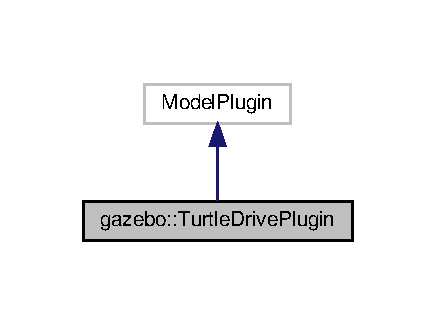
\includegraphics[width=209pt]{d6/d21/classgazebo_1_1TurtleDrivePlugin__inherit__graph}
\end{center}
\end{figure}


Collaboration diagram for gazebo\+:\+:Turtle\+Drive\+Plugin\+:\nopagebreak
\begin{figure}[H]
\begin{center}
\leavevmode
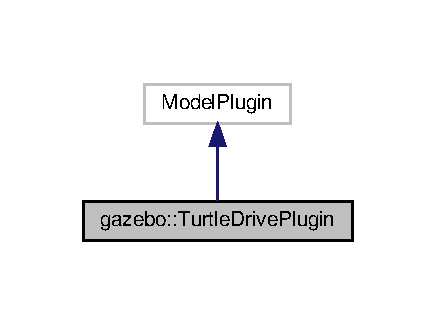
\includegraphics[width=209pt]{da/d2c/classgazebo_1_1TurtleDrivePlugin__coll__graph}
\end{center}
\end{figure}
\subsection*{Public Member Functions}
\begin{DoxyCompactItemize}
\item 
\mbox{\Hypertarget{classgazebo_1_1TurtleDrivePlugin_afde78faf88cde0df02bf1c8780777ba7}\label{classgazebo_1_1TurtleDrivePlugin_afde78faf88cde0df02bf1c8780777ba7}} 
void {\bfseries Load} (physics\+::\+Model\+Ptr \+\_\+parent, sdf\+::\+Element\+Ptr \+\_\+sdf)
\item 
\mbox{\Hypertarget{classgazebo_1_1TurtleDrivePlugin_a7eec7e21f3378aed676cc546692c55db}\label{classgazebo_1_1TurtleDrivePlugin_a7eec7e21f3378aed676cc546692c55db}} 
void {\bfseries callback\+\_\+wheel\+\_\+cmd} (nuturtlebot\+::\+Wheel\+Commands\+::\+Const\+Ptr data)
\item 
\mbox{\Hypertarget{classgazebo_1_1TurtleDrivePlugin_afb0469767e16f4d12e1c854acf43299a}\label{classgazebo_1_1TurtleDrivePlugin_afb0469767e16f4d12e1c854acf43299a}} 
void {\bfseries On\+Update} ()
\end{DoxyCompactItemize}


The documentation for this class was generated from the following file\+:\begin{DoxyCompactItemize}
\item 
nuturtle\+\_\+gazebo/src/turtle\+\_\+drive\+\_\+plugin.\+cpp\end{DoxyCompactItemize}

\hypertarget{structrigid2d_1_1Twist2D}{}\section{rigid2d\+:\+:Twist2D Struct Reference}
\label{structrigid2d_1_1Twist2D}\index{rigid2d\+::\+Twist2D@{rigid2d\+::\+Twist2D}}


A 2-\/\+Dimensional Twist.  




{\ttfamily \#include $<$rigid2d.\+hpp$>$}

\subsection*{Public Member Functions}
\begin{DoxyCompactItemize}
\item 
\mbox{\Hypertarget{structrigid2d_1_1Twist2D_a8a317315c9dc111b01e0f3c53af072b4}\label{structrigid2d_1_1Twist2D_a8a317315c9dc111b01e0f3c53af072b4}} 
\hyperlink{structrigid2d_1_1Twist2D_a8a317315c9dc111b01e0f3c53af072b4}{Twist2D} ()
\begin{DoxyCompactList}\small\item\em create an empty twist \end{DoxyCompactList}\item 
\hyperlink{structrigid2d_1_1Twist2D_a957e7c727d48e4d2b3f6c2390533e1bb}{Twist2D} (double ang, double linx, double liny)
\begin{DoxyCompactList}\small\item\em create a twist \end{DoxyCompactList}\item 
\hyperlink{structrigid2d_1_1Twist2D}{Twist2D} \hyperlink{structrigid2d_1_1Twist2D_ad5fb3449c63fceb7519c89ac84d3546e}{scale\+Twist} (double dt)
\begin{DoxyCompactList}\small\item\em scale this twist based on the current unit time \end{DoxyCompactList}\end{DoxyCompactItemize}
\subsection*{Public Attributes}
\begin{DoxyCompactItemize}
\item 
\mbox{\Hypertarget{structrigid2d_1_1Twist2D_ad556d2a04f31e2c5d8f4b45484782429}\label{structrigid2d_1_1Twist2D_ad556d2a04f31e2c5d8f4b45484782429}} 
double {\bfseries wz} = 0.\+0
\item 
\mbox{\Hypertarget{structrigid2d_1_1Twist2D_a95d7a5655df76416261f48346f549700}\label{structrigid2d_1_1Twist2D_a95d7a5655df76416261f48346f549700}} 
double {\bfseries vx} = 0.\+0
\item 
\mbox{\Hypertarget{structrigid2d_1_1Twist2D_abe86f0f1d0c00e42e5b388ca676e43dd}\label{structrigid2d_1_1Twist2D_abe86f0f1d0c00e42e5b388ca676e43dd}} 
double {\bfseries vy} = 0.\+0
\end{DoxyCompactItemize}


\subsection{Detailed Description}
A 2-\/\+Dimensional Twist. 

\subsection{Constructor \& Destructor Documentation}
\mbox{\Hypertarget{structrigid2d_1_1Twist2D_a957e7c727d48e4d2b3f6c2390533e1bb}\label{structrigid2d_1_1Twist2D_a957e7c727d48e4d2b3f6c2390533e1bb}} 
\index{rigid2d\+::\+Twist2D@{rigid2d\+::\+Twist2D}!Twist2D@{Twist2D}}
\index{Twist2D@{Twist2D}!rigid2d\+::\+Twist2D@{rigid2d\+::\+Twist2D}}
\subsubsection{\texorpdfstring{Twist2\+D()}{Twist2D()}}
{\footnotesize\ttfamily rigid2d\+::\+Twist2\+D\+::\+Twist2D (\begin{DoxyParamCaption}\item[{double}]{ang,  }\item[{double}]{linx,  }\item[{double}]{liny }\end{DoxyParamCaption})}



create a twist 


\begin{DoxyParams}{Parameters}
{\em ang} & -\/ the angular component \\
\hline
{\em xlin} & -\/ the x velocity component \\
\hline
{\em ylin} & -\/ the y velocity component \\
\hline
\end{DoxyParams}


\subsection{Member Function Documentation}
\mbox{\Hypertarget{structrigid2d_1_1Twist2D_ad5fb3449c63fceb7519c89ac84d3546e}\label{structrigid2d_1_1Twist2D_ad5fb3449c63fceb7519c89ac84d3546e}} 
\index{rigid2d\+::\+Twist2D@{rigid2d\+::\+Twist2D}!scale\+Twist@{scale\+Twist}}
\index{scale\+Twist@{scale\+Twist}!rigid2d\+::\+Twist2D@{rigid2d\+::\+Twist2D}}
\subsubsection{\texorpdfstring{scale\+Twist()}{scaleTwist()}}
{\footnotesize\ttfamily \hyperlink{structrigid2d_1_1Twist2D}{Twist2D} rigid2d\+::\+Twist2\+D\+::scale\+Twist (\begin{DoxyParamCaption}\item[{double}]{dt }\end{DoxyParamCaption})}



scale this twist based on the current unit time 


\begin{DoxyParams}{Parameters}
{\em dt} & -\/ the unit time \\
\hline
\end{DoxyParams}
\begin{DoxyReturn}{Returns}
this twist scaled by dt to 
\end{DoxyReturn}


The documentation for this struct was generated from the following files\+:\begin{DoxyCompactItemize}
\item 
rigid2d/include/rigid2d/\hyperlink{rigid2d_8hpp}{rigid2d.\+hpp}\item 
rigid2d/src/rigid2d/\hyperlink{rigid2d_8cpp}{rigid2d.\+cpp}\end{DoxyCompactItemize}

\hypertarget{structrigid2d_1_1Vector2D}{}\section{rigid2d\+:\+:Vector2D Struct Reference}
\label{structrigid2d_1_1Vector2D}\index{rigid2d\+::\+Vector2D@{rigid2d\+::\+Vector2D}}


A 2-\/\+Dimensional Vector.  




{\ttfamily \#include $<$rigid2d.\+hpp$>$}

\subsection*{Public Member Functions}
\begin{DoxyCompactItemize}
\item 
\mbox{\Hypertarget{structrigid2d_1_1Vector2D_aa268d230fdd3ddc7b5f89e6277ee60da}\label{structrigid2d_1_1Vector2D_aa268d230fdd3ddc7b5f89e6277ee60da}} 
\hyperlink{structrigid2d_1_1Vector2D_aa268d230fdd3ddc7b5f89e6277ee60da}{Vector2D} ()
\begin{DoxyCompactList}\small\item\em create an empty vector \end{DoxyCompactList}\item 
\hyperlink{structrigid2d_1_1Vector2D_a26d3fdc99cc873ff8785a70b7f379463}{Vector2D} (double xcomp, double ycomp)
\begin{DoxyCompactList}\small\item\em create a vector \end{DoxyCompactList}\item 
\hyperlink{structrigid2d_1_1Vector2D}{Vector2D} \hyperlink{structrigid2d_1_1Vector2D_a6534f1075f8f3338261331c954b449b2}{normalize} () const
\begin{DoxyCompactList}\small\item\em output a unit vector corresponding to the \mbox{[}xcomponent ycomponent\mbox{]} \end{DoxyCompactList}\item 
double \hyperlink{structrigid2d_1_1Vector2D_afe2117dc061b3f09c890ac13dd59c345}{length} () const
\begin{DoxyCompactList}\small\item\em calculate the length of the vector based on the components \end{DoxyCompactList}\item 
double \hyperlink{structrigid2d_1_1Vector2D_a61ec013677fd4439fa21c35656fe7256}{angle} () const
\begin{DoxyCompactList}\small\item\em calculate the angle of the vector based on the components \end{DoxyCompactList}\item 
double \hyperlink{structrigid2d_1_1Vector2D_a929393171d0ac3cc0a3f438d9a2c9cf1}{distance} (\hyperlink{structrigid2d_1_1Vector2D}{Vector2D} vec) const
\begin{DoxyCompactList}\small\item\em calculate the distance between this vector and another \end{DoxyCompactList}\item 
\hyperlink{structrigid2d_1_1Vector2D}{Vector2D} \& \hyperlink{structrigid2d_1_1Vector2D_aa17e3466179575f598b77153cbfea9e6}{operator+=} (const \hyperlink{structrigid2d_1_1Vector2D}{Vector2D} \&rhs)
\begin{DoxyCompactList}\small\item\em add this vector with another and store the result in this object \end{DoxyCompactList}\item 
\hyperlink{structrigid2d_1_1Vector2D}{Vector2D} \& \hyperlink{structrigid2d_1_1Vector2D_a8ef35cca4a51ecd76bee8b8dca5e3a63}{operator-\/=} (const \hyperlink{structrigid2d_1_1Vector2D}{Vector2D} \&rhs)
\begin{DoxyCompactList}\small\item\em subtract this vector with another and store the result in this object \end{DoxyCompactList}\item 
\hyperlink{structrigid2d_1_1Vector2D}{Vector2D} \& \hyperlink{structrigid2d_1_1Vector2D_a0da46fe8a92fcb6ecea09425c6ead294}{operator$\ast$=} (const \hyperlink{structrigid2d_1_1Vector2D}{Vector2D} \&rhs)
\begin{DoxyCompactList}\small\item\em multiply(scalar) this vector with another and store the result in this object \end{DoxyCompactList}\end{DoxyCompactItemize}
\subsection*{Public Attributes}
\begin{DoxyCompactItemize}
\item 
\mbox{\Hypertarget{structrigid2d_1_1Vector2D_a1876d655fe2da548c4813777c450845c}\label{structrigid2d_1_1Vector2D_a1876d655fe2da548c4813777c450845c}} 
double \hyperlink{structrigid2d_1_1Vector2D_a1876d655fe2da548c4813777c450845c}{x}
\begin{DoxyCompactList}\small\item\em x val of vector \end{DoxyCompactList}\item 
\mbox{\Hypertarget{structrigid2d_1_1Vector2D_aa814ea37ffe4a161b0020609580e4d17}\label{structrigid2d_1_1Vector2D_aa814ea37ffe4a161b0020609580e4d17}} 
double \hyperlink{structrigid2d_1_1Vector2D_aa814ea37ffe4a161b0020609580e4d17}{y}
\begin{DoxyCompactList}\small\item\em y val of vector \end{DoxyCompactList}\end{DoxyCompactItemize}


\subsection{Detailed Description}
A 2-\/\+Dimensional Vector. 

\subsection{Constructor \& Destructor Documentation}
\mbox{\Hypertarget{structrigid2d_1_1Vector2D_a26d3fdc99cc873ff8785a70b7f379463}\label{structrigid2d_1_1Vector2D_a26d3fdc99cc873ff8785a70b7f379463}} 
\index{rigid2d\+::\+Vector2D@{rigid2d\+::\+Vector2D}!Vector2D@{Vector2D}}
\index{Vector2D@{Vector2D}!rigid2d\+::\+Vector2D@{rigid2d\+::\+Vector2D}}
\subsubsection{\texorpdfstring{Vector2\+D()}{Vector2D()}}
{\footnotesize\ttfamily rigid2d\+::\+Vector2\+D\+::\+Vector2D (\begin{DoxyParamCaption}\item[{double}]{xcomp,  }\item[{double}]{ycomp }\end{DoxyParamCaption})}



create a vector 


\begin{DoxyParams}{Parameters}
{\em xcomp} & -\/ the x vector component \\
\hline
{\em ycomp} & -\/ the y vector component \\
\hline
\end{DoxyParams}


\subsection{Member Function Documentation}
\mbox{\Hypertarget{structrigid2d_1_1Vector2D_a61ec013677fd4439fa21c35656fe7256}\label{structrigid2d_1_1Vector2D_a61ec013677fd4439fa21c35656fe7256}} 
\index{rigid2d\+::\+Vector2D@{rigid2d\+::\+Vector2D}!angle@{angle}}
\index{angle@{angle}!rigid2d\+::\+Vector2D@{rigid2d\+::\+Vector2D}}
\subsubsection{\texorpdfstring{angle()}{angle()}}
{\footnotesize\ttfamily double rigid2d\+::\+Vector2\+D\+::angle (\begin{DoxyParamCaption}{ }\end{DoxyParamCaption}) const}



calculate the angle of the vector based on the components 

\begin{DoxyReturn}{Returns}
the angle of this vector in degrees 
\end{DoxyReturn}
\mbox{\Hypertarget{structrigid2d_1_1Vector2D_a929393171d0ac3cc0a3f438d9a2c9cf1}\label{structrigid2d_1_1Vector2D_a929393171d0ac3cc0a3f438d9a2c9cf1}} 
\index{rigid2d\+::\+Vector2D@{rigid2d\+::\+Vector2D}!distance@{distance}}
\index{distance@{distance}!rigid2d\+::\+Vector2D@{rigid2d\+::\+Vector2D}}
\subsubsection{\texorpdfstring{distance()}{distance()}}
{\footnotesize\ttfamily double rigid2d\+::\+Vector2\+D\+::distance (\begin{DoxyParamCaption}\item[{\hyperlink{structrigid2d_1_1Vector2D}{Vector2D}}]{vec }\end{DoxyParamCaption}) const}



calculate the distance between this vector and another 


\begin{DoxyParams}{Parameters}
{\em vec} & -\/ vector to find the distance to \\
\hline
\end{DoxyParams}
\begin{DoxyReturn}{Returns}
the distance between the two vectors 
\end{DoxyReturn}
\mbox{\Hypertarget{structrigid2d_1_1Vector2D_afe2117dc061b3f09c890ac13dd59c345}\label{structrigid2d_1_1Vector2D_afe2117dc061b3f09c890ac13dd59c345}} 
\index{rigid2d\+::\+Vector2D@{rigid2d\+::\+Vector2D}!length@{length}}
\index{length@{length}!rigid2d\+::\+Vector2D@{rigid2d\+::\+Vector2D}}
\subsubsection{\texorpdfstring{length()}{length()}}
{\footnotesize\ttfamily double rigid2d\+::\+Vector2\+D\+::length (\begin{DoxyParamCaption}{ }\end{DoxyParamCaption}) const}



calculate the length of the vector based on the components 

\begin{DoxyReturn}{Returns}
the length of this vector 
\end{DoxyReturn}
\mbox{\Hypertarget{structrigid2d_1_1Vector2D_a6534f1075f8f3338261331c954b449b2}\label{structrigid2d_1_1Vector2D_a6534f1075f8f3338261331c954b449b2}} 
\index{rigid2d\+::\+Vector2D@{rigid2d\+::\+Vector2D}!normalize@{normalize}}
\index{normalize@{normalize}!rigid2d\+::\+Vector2D@{rigid2d\+::\+Vector2D}}
\subsubsection{\texorpdfstring{normalize()}{normalize()}}
{\footnotesize\ttfamily \hyperlink{structrigid2d_1_1Vector2D}{Vector2D} rigid2d\+::\+Vector2\+D\+::normalize (\begin{DoxyParamCaption}{ }\end{DoxyParamCaption}) const}



output a unit vector corresponding to the \mbox{[}xcomponent ycomponent\mbox{]} 

\begin{DoxyReturn}{Returns}
the unit vector corresponding to the current x and y values of the \hyperlink{structrigid2d_1_1Vector2D}{Vector2D} 
\end{DoxyReturn}
\mbox{\Hypertarget{structrigid2d_1_1Vector2D_a0da46fe8a92fcb6ecea09425c6ead294}\label{structrigid2d_1_1Vector2D_a0da46fe8a92fcb6ecea09425c6ead294}} 
\index{rigid2d\+::\+Vector2D@{rigid2d\+::\+Vector2D}!operator$\ast$=@{operator$\ast$=}}
\index{operator$\ast$=@{operator$\ast$=}!rigid2d\+::\+Vector2D@{rigid2d\+::\+Vector2D}}
\subsubsection{\texorpdfstring{operator$\ast$=()}{operator*=()}}
{\footnotesize\ttfamily \hyperlink{structrigid2d_1_1Vector2D}{Vector2D} \& rigid2d\+::\+Vector2\+D\+::operator$\ast$= (\begin{DoxyParamCaption}\item[{const \hyperlink{structrigid2d_1_1Vector2D}{Vector2D} \&}]{rhs }\end{DoxyParamCaption})}



multiply(scalar) this vector with another and store the result in this object 


\begin{DoxyParams}{Parameters}
{\em rhs} & -\/ the vector to multiply by \\
\hline
\end{DoxyParams}
\begin{DoxyReturn}{Returns}
a reference to the newly transformed operator 
\end{DoxyReturn}
\mbox{\Hypertarget{structrigid2d_1_1Vector2D_aa17e3466179575f598b77153cbfea9e6}\label{structrigid2d_1_1Vector2D_aa17e3466179575f598b77153cbfea9e6}} 
\index{rigid2d\+::\+Vector2D@{rigid2d\+::\+Vector2D}!operator+=@{operator+=}}
\index{operator+=@{operator+=}!rigid2d\+::\+Vector2D@{rigid2d\+::\+Vector2D}}
\subsubsection{\texorpdfstring{operator+=()}{operator+=()}}
{\footnotesize\ttfamily \hyperlink{structrigid2d_1_1Vector2D}{Vector2D} \& rigid2d\+::\+Vector2\+D\+::operator+= (\begin{DoxyParamCaption}\item[{const \hyperlink{structrigid2d_1_1Vector2D}{Vector2D} \&}]{rhs }\end{DoxyParamCaption})}



add this vector with another and store the result in this object 


\begin{DoxyParams}{Parameters}
{\em rhs} & -\/ the vector to add by \\
\hline
\end{DoxyParams}
\begin{DoxyReturn}{Returns}
a reference to the newly transformed operator 
\end{DoxyReturn}
\mbox{\Hypertarget{structrigid2d_1_1Vector2D_a8ef35cca4a51ecd76bee8b8dca5e3a63}\label{structrigid2d_1_1Vector2D_a8ef35cca4a51ecd76bee8b8dca5e3a63}} 
\index{rigid2d\+::\+Vector2D@{rigid2d\+::\+Vector2D}!operator-\/=@{operator-\/=}}
\index{operator-\/=@{operator-\/=}!rigid2d\+::\+Vector2D@{rigid2d\+::\+Vector2D}}
\subsubsection{\texorpdfstring{operator-\/=()}{operator-=()}}
{\footnotesize\ttfamily \hyperlink{structrigid2d_1_1Vector2D}{Vector2D} \& rigid2d\+::\+Vector2\+D\+::operator-\/= (\begin{DoxyParamCaption}\item[{const \hyperlink{structrigid2d_1_1Vector2D}{Vector2D} \&}]{rhs }\end{DoxyParamCaption})}



subtract this vector with another and store the result in this object 


\begin{DoxyParams}{Parameters}
{\em rhs} & -\/ the vector to subtract by \\
\hline
\end{DoxyParams}
\begin{DoxyReturn}{Returns}
a reference to the newly transformed operator 
\end{DoxyReturn}


The documentation for this struct was generated from the following files\+:\begin{DoxyCompactItemize}
\item 
rigid2d/include/rigid2d/\hyperlink{rigid2d_8hpp}{rigid2d.\+hpp}\item 
rigid2d/src/rigid2d/\hyperlink{rigid2d_8cpp}{rigid2d.\+cpp}\end{DoxyCompactItemize}

\hypertarget{classrigid2d_1_1Waypoints}{}\section{rigid2d\+:\+:Waypoints Class Reference}
\label{classrigid2d_1_1Waypoints}\index{rigid2d\+::\+Waypoints@{rigid2d\+::\+Waypoints}}
\subsection*{Public Member Functions}
\begin{DoxyCompactItemize}
\item 
\mbox{\Hypertarget{classrigid2d_1_1Waypoints_a8e7579d65c588966c0f53866a73fee43}\label{classrigid2d_1_1Waypoints_a8e7579d65c588966c0f53866a73fee43}} 
\hyperlink{classrigid2d_1_1Waypoints_a8e7579d65c588966c0f53866a73fee43}{Waypoints} ()
\begin{DoxyCompactList}\small\item\em Use defualt values for parameters. \end{DoxyCompactList}\item 
\mbox{\Hypertarget{classrigid2d_1_1Waypoints_a022820eb64ed86a33d3677f9880193fa}\label{classrigid2d_1_1Waypoints_a022820eb64ed86a33d3677f9880193fa}} 
\hyperlink{classrigid2d_1_1Waypoints_a022820eb64ed86a33d3677f9880193fa}{Waypoints} (std\+::vector$<$ \hyperlink{structrigid2d_1_1Vector2D}{Vector2D} $>$ points, int r, double vlim, double alim)
\begin{DoxyCompactList}\small\item\em Use a custom waypoint string. \end{DoxyCompactList}\item 
\hyperlink{structrigid2d_1_1Twist2D}{Twist2D} \hyperlink{classrigid2d_1_1Waypoints_acf263076e58543a95391476650f84c85}{next\+Waypoint} (\hyperlink{structrigid2d_1_1Pose2D}{Pose2D} pos)
\begin{DoxyCompactList}\small\item\em Method to calculate the next velocity command given the current target waypoint. \end{DoxyCompactList}\item 
void \hyperlink{classrigid2d_1_1Waypoints_a7ab69beb06eae9eb6f8c110748a6454f}{set\+Vlims} (double lin, double ang)
\begin{DoxyCompactList}\small\item\em set the internal velocity limits \end{DoxyCompactList}\item 
void \hyperlink{classrigid2d_1_1Waypoints_a00beb3a1c2d2f3b24e2a107221a8fa9c}{set\+Rate} (int r)
\begin{DoxyCompactList}\small\item\em set the internal rate \end{DoxyCompactList}\item 
void \hyperlink{classrigid2d_1_1Waypoints_a056d60e2226093ab70f218f6088e0bd9}{set\+Thresholds} (double alim, double tlim)
\begin{DoxyCompactList}\small\item\em set the angular and distance thresholds \end{DoxyCompactList}\item 
void \hyperlink{classrigid2d_1_1Waypoints_a2b29f071318d349824d8b704d01e32bf}{set\+Gains} (double p)
\begin{DoxyCompactList}\small\item\em set the controls gains \end{DoxyCompactList}\item 
\hyperlink{structrigid2d_1_1Vector2D}{Vector2D} \hyperlink{classrigid2d_1_1Waypoints_a2d50627bc6c0b74b247bebe0bdbcec38}{get\+Target} ()
\begin{DoxyCompactList}\small\item\em get the current target \end{DoxyCompactList}\item 
int \hyperlink{classrigid2d_1_1Waypoints_a75955fd8b5eb08a4da95668e4fb6aee6}{get\+Cycles} ()
\begin{DoxyCompactList}\small\item\em get the number of completed cycles \end{DoxyCompactList}\end{DoxyCompactItemize}


\subsection{Member Function Documentation}
\mbox{\Hypertarget{classrigid2d_1_1Waypoints_a75955fd8b5eb08a4da95668e4fb6aee6}\label{classrigid2d_1_1Waypoints_a75955fd8b5eb08a4da95668e4fb6aee6}} 
\index{rigid2d\+::\+Waypoints@{rigid2d\+::\+Waypoints}!get\+Cycles@{get\+Cycles}}
\index{get\+Cycles@{get\+Cycles}!rigid2d\+::\+Waypoints@{rigid2d\+::\+Waypoints}}
\subsubsection{\texorpdfstring{get\+Cycles()}{getCycles()}}
{\footnotesize\ttfamily int rigid2d\+::\+Waypoints\+::get\+Cycles (\begin{DoxyParamCaption}{ }\end{DoxyParamCaption})}



get the number of completed cycles 

\begin{DoxyReturn}{Returns}
the number of completed cycles 
\end{DoxyReturn}
\mbox{\Hypertarget{classrigid2d_1_1Waypoints_a2d50627bc6c0b74b247bebe0bdbcec38}\label{classrigid2d_1_1Waypoints_a2d50627bc6c0b74b247bebe0bdbcec38}} 
\index{rigid2d\+::\+Waypoints@{rigid2d\+::\+Waypoints}!get\+Target@{get\+Target}}
\index{get\+Target@{get\+Target}!rigid2d\+::\+Waypoints@{rigid2d\+::\+Waypoints}}
\subsubsection{\texorpdfstring{get\+Target()}{getTarget()}}
{\footnotesize\ttfamily \hyperlink{structrigid2d_1_1Vector2D}{Vector2D} rigid2d\+::\+Waypoints\+::get\+Target (\begin{DoxyParamCaption}{ }\end{DoxyParamCaption})}



get the current target 

\begin{DoxyReturn}{Returns}
the current target 
\end{DoxyReturn}
\mbox{\Hypertarget{classrigid2d_1_1Waypoints_acf263076e58543a95391476650f84c85}\label{classrigid2d_1_1Waypoints_acf263076e58543a95391476650f84c85}} 
\index{rigid2d\+::\+Waypoints@{rigid2d\+::\+Waypoints}!next\+Waypoint@{next\+Waypoint}}
\index{next\+Waypoint@{next\+Waypoint}!rigid2d\+::\+Waypoints@{rigid2d\+::\+Waypoints}}
\subsubsection{\texorpdfstring{next\+Waypoint()}{nextWaypoint()}}
{\footnotesize\ttfamily \hyperlink{structrigid2d_1_1Twist2D}{Twist2D} rigid2d\+::\+Waypoints\+::next\+Waypoint (\begin{DoxyParamCaption}\item[{\hyperlink{structrigid2d_1_1Pose2D}{Pose2D}}]{pos }\end{DoxyParamCaption})}



Method to calculate the next velocity command given the current target waypoint. 


\begin{DoxyParams}{Parameters}
{\em pos} & -\/ the current pose of the robot \\
\hline
\end{DoxyParams}
\begin{DoxyReturn}{Returns}
The velocity command to reach the next waypoint 
\end{DoxyReturn}
\mbox{\Hypertarget{classrigid2d_1_1Waypoints_a2b29f071318d349824d8b704d01e32bf}\label{classrigid2d_1_1Waypoints_a2b29f071318d349824d8b704d01e32bf}} 
\index{rigid2d\+::\+Waypoints@{rigid2d\+::\+Waypoints}!set\+Gains@{set\+Gains}}
\index{set\+Gains@{set\+Gains}!rigid2d\+::\+Waypoints@{rigid2d\+::\+Waypoints}}
\subsubsection{\texorpdfstring{set\+Gains()}{setGains()}}
{\footnotesize\ttfamily void rigid2d\+::\+Waypoints\+::set\+Gains (\begin{DoxyParamCaption}\item[{double}]{p }\end{DoxyParamCaption})}



set the controls gains 


\begin{DoxyParams}{Parameters}
{\em p} & -\/ the proportional control gain \\
\hline
\end{DoxyParams}
\mbox{\Hypertarget{classrigid2d_1_1Waypoints_a00beb3a1c2d2f3b24e2a107221a8fa9c}\label{classrigid2d_1_1Waypoints_a00beb3a1c2d2f3b24e2a107221a8fa9c}} 
\index{rigid2d\+::\+Waypoints@{rigid2d\+::\+Waypoints}!set\+Rate@{set\+Rate}}
\index{set\+Rate@{set\+Rate}!rigid2d\+::\+Waypoints@{rigid2d\+::\+Waypoints}}
\subsubsection{\texorpdfstring{set\+Rate()}{setRate()}}
{\footnotesize\ttfamily void rigid2d\+::\+Waypoints\+::set\+Rate (\begin{DoxyParamCaption}\item[{int}]{r }\end{DoxyParamCaption})}



set the internal rate 


\begin{DoxyParams}{Parameters}
{\em r} & -\/ the desired rate \\
\hline
\end{DoxyParams}
\mbox{\Hypertarget{classrigid2d_1_1Waypoints_a056d60e2226093ab70f218f6088e0bd9}\label{classrigid2d_1_1Waypoints_a056d60e2226093ab70f218f6088e0bd9}} 
\index{rigid2d\+::\+Waypoints@{rigid2d\+::\+Waypoints}!set\+Thresholds@{set\+Thresholds}}
\index{set\+Thresholds@{set\+Thresholds}!rigid2d\+::\+Waypoints@{rigid2d\+::\+Waypoints}}
\subsubsection{\texorpdfstring{set\+Thresholds()}{setThresholds()}}
{\footnotesize\ttfamily void rigid2d\+::\+Waypoints\+::set\+Thresholds (\begin{DoxyParamCaption}\item[{double}]{alim,  }\item[{double}]{tlim }\end{DoxyParamCaption})}



set the angular and distance thresholds 


\begin{DoxyParams}{Parameters}
{\em alim} & -\/ the angular position threshold \\
\hline
{\em tlim} & -\/ the translation position threshold \\
\hline
\end{DoxyParams}
\mbox{\Hypertarget{classrigid2d_1_1Waypoints_a7ab69beb06eae9eb6f8c110748a6454f}\label{classrigid2d_1_1Waypoints_a7ab69beb06eae9eb6f8c110748a6454f}} 
\index{rigid2d\+::\+Waypoints@{rigid2d\+::\+Waypoints}!set\+Vlims@{set\+Vlims}}
\index{set\+Vlims@{set\+Vlims}!rigid2d\+::\+Waypoints@{rigid2d\+::\+Waypoints}}
\subsubsection{\texorpdfstring{set\+Vlims()}{setVlims()}}
{\footnotesize\ttfamily void rigid2d\+::\+Waypoints\+::set\+Vlims (\begin{DoxyParamCaption}\item[{double}]{lin,  }\item[{double}]{ang }\end{DoxyParamCaption})}



set the internal velocity limits 


\begin{DoxyParams}{Parameters}
{\em lin} & -\/ the linear velocity limit \\
\hline
{\em ang} & -\/ the angular velocity limit \\
\hline
\end{DoxyParams}


The documentation for this class was generated from the following files\+:\begin{DoxyCompactItemize}
\item 
rigid2d/include/rigid2d/\hyperlink{waypoints_8hpp}{waypoints.\+hpp}\item 
rigid2d/src/rigid2d/\hyperlink{waypoints_8cpp}{waypoints.\+cpp}\end{DoxyCompactItemize}

\hypertarget{structrigid2d_1_1WheelVelocities}{}\section{rigid2d\+:\+:Wheel\+Velocities Struct Reference}
\label{structrigid2d_1_1WheelVelocities}\index{rigid2d\+::\+Wheel\+Velocities@{rigid2d\+::\+Wheel\+Velocities}}


Wheel velocities for a diff drive robot.  




{\ttfamily \#include $<$diff\+\_\+drive.\+hpp$>$}

\subsection*{Public Member Functions}
\begin{DoxyCompactItemize}
\item 
\mbox{\Hypertarget{structrigid2d_1_1WheelVelocities_a406eb6ddee2a8cfff2e88359462cd1c3}\label{structrigid2d_1_1WheelVelocities_a406eb6ddee2a8cfff2e88359462cd1c3}} 
\hyperlink{structrigid2d_1_1WheelVelocities_a406eb6ddee2a8cfff2e88359462cd1c3}{Wheel\+Velocities} ()
\begin{DoxyCompactList}\small\item\em sets wheel velocities to zero \end{DoxyCompactList}\item 
\mbox{\Hypertarget{structrigid2d_1_1WheelVelocities_a580b7a8bfb68b61d5423adc3de5de4a9}\label{structrigid2d_1_1WheelVelocities_a580b7a8bfb68b61d5423adc3de5de4a9}} 
\hyperlink{structrigid2d_1_1WheelVelocities_a580b7a8bfb68b61d5423adc3de5de4a9}{Wheel\+Velocities} (double left, double right)
\begin{DoxyCompactList}\small\item\em sets wheel velocity parameters to specified values \end{DoxyCompactList}\end{DoxyCompactItemize}
\subsection*{Public Attributes}
\begin{DoxyCompactItemize}
\item 
\mbox{\Hypertarget{structrigid2d_1_1WheelVelocities_a647f6d1dd95af0323780c8b7d639ccf3}\label{structrigid2d_1_1WheelVelocities_a647f6d1dd95af0323780c8b7d639ccf3}} 
double {\bfseries ur} = 0
\item 
\mbox{\Hypertarget{structrigid2d_1_1WheelVelocities_a7e2524297e82e99d40e575633184d060}\label{structrigid2d_1_1WheelVelocities_a7e2524297e82e99d40e575633184d060}} 
double {\bfseries ul} = 0
\end{DoxyCompactItemize}


\subsection{Detailed Description}
Wheel velocities for a diff drive robot. 

The documentation for this struct was generated from the following files\+:\begin{DoxyCompactItemize}
\item 
rigid2d/include/rigid2d/\hyperlink{diff__drive_8hpp}{diff\+\_\+drive.\+hpp}\item 
rigid2d/src/rigid2d/\hyperlink{diff__drive_8cpp}{diff\+\_\+drive.\+cpp}\end{DoxyCompactItemize}

\chapter{File Documentation}
\hypertarget{cylinder__detect_8hpp}{}\section{nuslam/include/nuslam/cylinder\+\_\+detect.hpp File Reference}
\label{cylinder__detect_8hpp}\index{nuslam/include/nuslam/cylinder\+\_\+detect.\+hpp@{nuslam/include/nuslam/cylinder\+\_\+detect.\+hpp}}


function to fit circles.  


{\ttfamily \#include $<$vector$>$}\newline
{\ttfamily \#include \char`\"{}rigid2d/rigid2d.\+hpp\char`\"{}}\newline
Include dependency graph for cylinder\+\_\+detect.\+hpp\+:\nopagebreak
\begin{figure}[H]
\begin{center}
\leavevmode
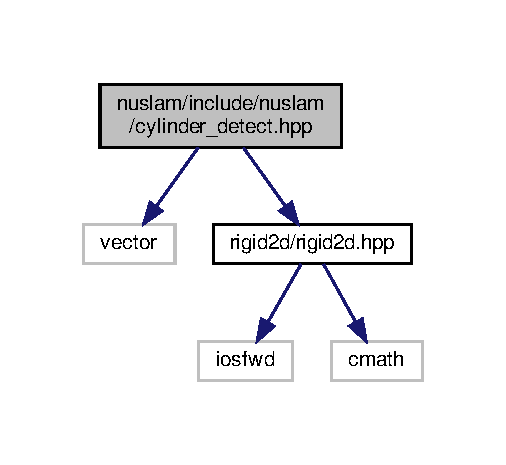
\includegraphics[width=243pt]{dd/d3a/cylinder__detect_8hpp__incl}
\end{center}
\end{figure}
This graph shows which files directly or indirectly include this file\+:\nopagebreak
\begin{figure}[H]
\begin{center}
\leavevmode
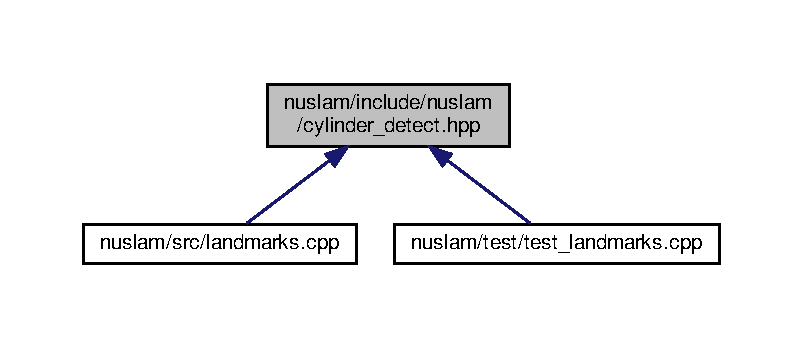
\includegraphics[width=350pt]{d9/d9e/cylinder__detect_8hpp__dep__incl}
\end{center}
\end{figure}
\subsection*{Functions}
\begin{DoxyCompactItemize}
\item 
std\+::vector$<$ double $>$ \hyperlink{cylinder__detect_8hpp_a5351498f6edb96444bf8d93c4f743793}{cylinder\+::fit\+\_\+circles} (std\+::vector$<$ \hyperlink{structrigid2d_1_1Vector2D}{rigid2d\+::\+Vector2D} $>$ cluster)
\begin{DoxyCompactList}\small\item\em function to fit a circle to a cluster of points \end{DoxyCompactList}\end{DoxyCompactItemize}


\subsection{Detailed Description}
function to fit circles. 



\subsection{Function Documentation}
\mbox{\Hypertarget{cylinder__detect_8hpp_file_a5351498f6edb96444bf8d93c4f743793}\label{cylinder__detect_8hpp_file_a5351498f6edb96444bf8d93c4f743793}} 
\index{cylinder\+\_\+detect.\+hpp@{cylinder\+\_\+detect.\+hpp}!fit\+\_\+circles@{fit\+\_\+circles}}
\index{fit\+\_\+circles@{fit\+\_\+circles}!cylinder\+\_\+detect.\+hpp@{cylinder\+\_\+detect.\+hpp}}
\subsubsection{\texorpdfstring{fit\+\_\+circles()}{fit\_circles()}}
{\footnotesize\ttfamily std\+::vector$<$ double $>$ cylinder\+::fit\+\_\+circles (\begin{DoxyParamCaption}\item[{std\+::vector$<$ \hyperlink{structrigid2d_1_1Vector2D}{rigid2d\+::\+Vector2D} $>$}]{cluster }\end{DoxyParamCaption})}



function to fit a circle to a cluster of points 


\begin{DoxyParams}{Parameters}
{\em cluster} & a vector of x,y points that are physically near each other \\
\hline
\end{DoxyParams}
\begin{DoxyReturn}{Returns}
circle\+\_\+params\+: a vector where the first two number are the cenroid coordinates and the third is the radius 
\end{DoxyReturn}

\hypertarget{ekf__slam_8hpp}{}\section{nuslam/include/nuslam/ekf\+\_\+slam.hpp File Reference}
\label{ekf__slam_8hpp}\index{nuslam/include/nuslam/ekf\+\_\+slam.\+hpp@{nuslam/include/nuslam/ekf\+\_\+slam.\+hpp}}


Library to contain S\+L\+AM class and supporting functions.  


{\ttfamily \#include $<$eigen3/\+Eigen/\+Dense$>$}\newline
{\ttfamily \#include $<$vector$>$}\newline
{\ttfamily \#include $<$iostream$>$}\newline
{\ttfamily \#include \char`\"{}geometry\+\_\+msgs/\+Point.\+h\char`\"{}}\newline
{\ttfamily \#include \char`\"{}rigid2d/rigid2d.\+hpp\char`\"{}}\newline
Include dependency graph for ekf\+\_\+slam.\+hpp\+:
\nopagebreak
\begin{figure}[H]
\begin{center}
\leavevmode
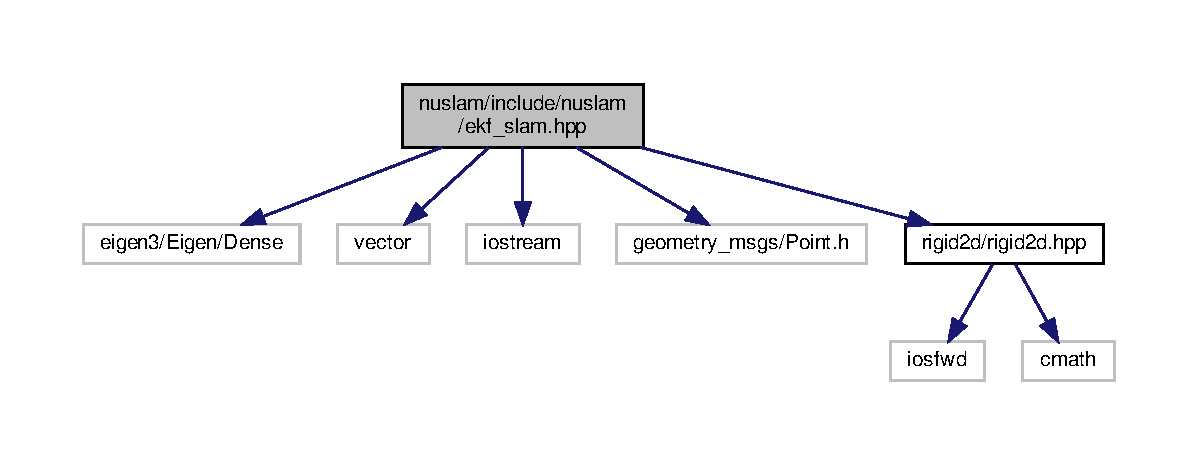
\includegraphics[width=350pt]{d7/dc4/ekf__slam_8hpp__incl}
\end{center}
\end{figure}
This graph shows which files directly or indirectly include this file\+:
\nopagebreak
\begin{figure}[H]
\begin{center}
\leavevmode
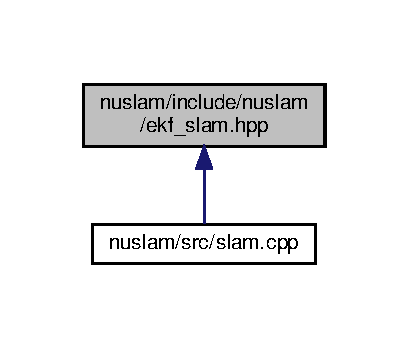
\includegraphics[width=196pt]{db/d24/ekf__slam_8hpp__dep__incl}
\end{center}
\end{figure}
\subsection*{Classes}
\begin{DoxyCompactItemize}
\item 
class \hyperlink{classekf__slam_1_1Slam}{ekf\+\_\+slam\+::\+Slam}
\end{DoxyCompactItemize}
\subsection*{Functions}
\begin{DoxyCompactItemize}
\item 
\mbox{\Hypertarget{ekf__slam_8hpp_a4db5cb1b575327c82d0bde88900522e7}\label{ekf__slam_8hpp_a4db5cb1b575327c82d0bde88900522e7}} 
double \hyperlink{ekf__slam_8hpp_a4db5cb1b575327c82d0bde88900522e7}{ekf\+\_\+slam\+::sample\+Normal\+Distribution} ()
\begin{DoxyCompactList}\small\item\em Draw a random value from a normal distribution. \end{DoxyCompactList}\end{DoxyCompactItemize}


\subsection{Detailed Description}
Library to contain S\+L\+AM class and supporting functions. 


\hypertarget{analysis_8cpp}{}\section{nuslam/src/analysis.cpp File Reference}
\label{analysis_8cpp}\index{nuslam/src/analysis.\+cpp@{nuslam/src/analysis.\+cpp}}


This node takes the information from gazebo and publishes it for debuggin S\+L\+AM node.  


{\ttfamily \#include $<$ros/ros.\+h$>$}\newline
{\ttfamily \#include $<$string.\+h$>$}\newline
{\ttfamily \#include $<$vector$>$}\newline
{\ttfamily \#include $<$tf2/\+Linear\+Math/\+Quaternion.\+h$>$}\newline
{\ttfamily \#include $<$tf2\+\_\+geometry\+\_\+msgs/tf2\+\_\+geometry\+\_\+msgs.\+h$>$}\newline
{\ttfamily \#include \char`\"{}gazebo\+\_\+msgs/\+Model\+States.\+h\char`\"{}}\newline
{\ttfamily \#include \char`\"{}geometry\+\_\+msgs/\+Point.\+h\char`\"{}}\newline
{\ttfamily \#include \char`\"{}geometry\+\_\+msgs/\+Pose.\+h\char`\"{}}\newline
{\ttfamily \#include \char`\"{}nuslam/\+Turtle\+Map.\+h\char`\"{}}\newline
{\ttfamily \#include \char`\"{}nav\+\_\+msgs/\+Path.\+h\char`\"{}}\newline
{\ttfamily \#include \char`\"{}rigid2d/rigid2d.\+hpp\char`\"{}}\newline
Include dependency graph for analysis.\+cpp\+:\nopagebreak
\begin{figure}[H]
\begin{center}
\leavevmode
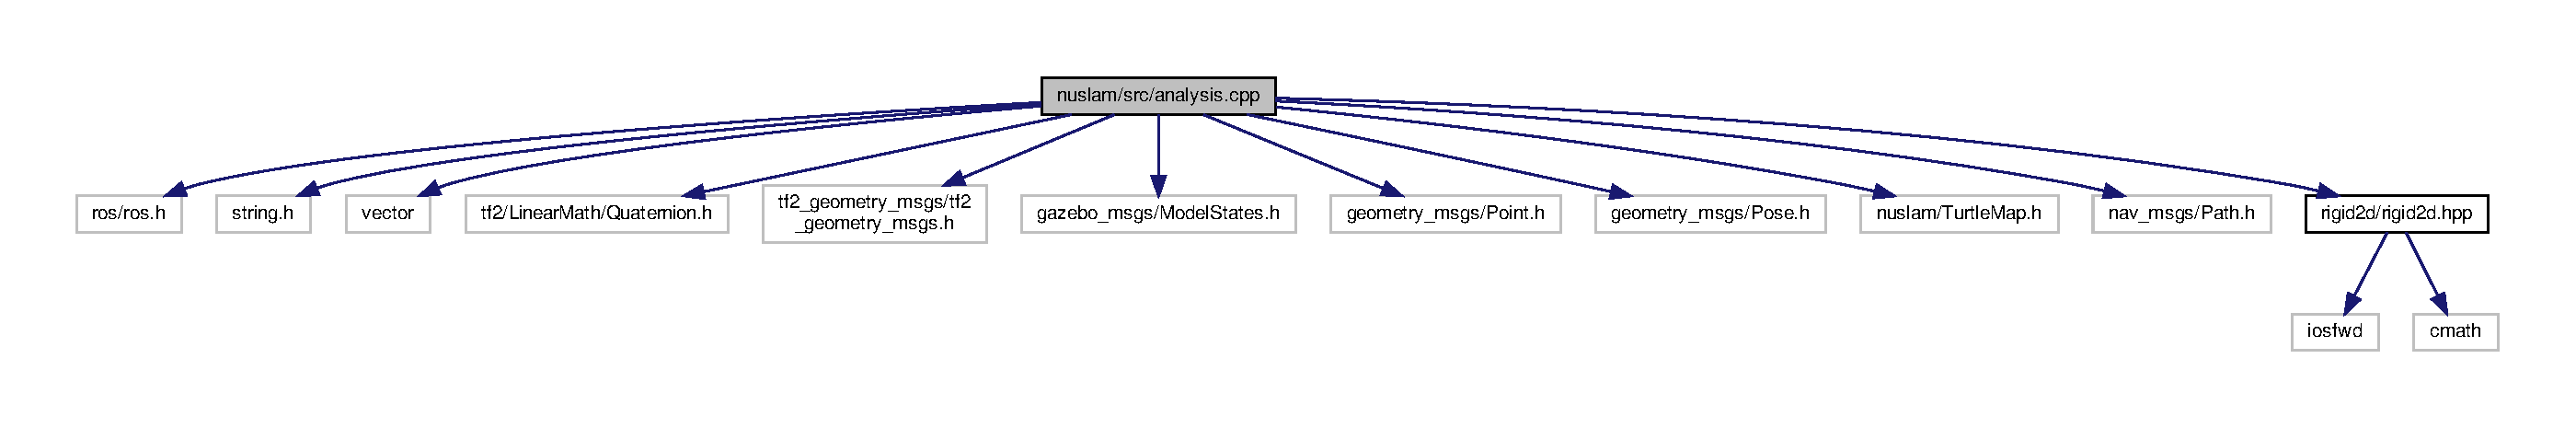
\includegraphics[width=350pt]{d5/dbb/analysis_8cpp__incl}
\end{center}
\end{figure}
\subsection*{Functions}
\begin{DoxyCompactItemize}
\item 
\mbox{\Hypertarget{analysis_8cpp_ab2abfd62ddd28e7ce8c819816d0ecce3}\label{analysis_8cpp_ab2abfd62ddd28e7ce8c819816d0ecce3}} 
void \hyperlink{analysis_8cpp_ab2abfd62ddd28e7ce8c819816d0ecce3}{callback\+\_\+gazebo\+\_\+data} (const gazebo\+\_\+msgs\+::\+Model\+States \&data)
\begin{DoxyCompactList}\small\item\em Convert gazebo data to Turtle\+Map format. \end{DoxyCompactList}\item 
\mbox{\Hypertarget{analysis_8cpp_a3c04138a5bfe5d72780bb7e82a18e627}\label{analysis_8cpp_a3c04138a5bfe5d72780bb7e82a18e627}} 
int \hyperlink{analysis_8cpp_a3c04138a5bfe5d72780bb7e82a18e627}{main} (int argc, char $\ast$$\ast$argv)
\begin{DoxyCompactList}\small\item\em main function \end{DoxyCompactList}\end{DoxyCompactItemize}
\subsection*{Variables}
\begin{DoxyCompactItemize}
\item 
\mbox{\Hypertarget{analysis_8cpp_af5ed1bf78a7815965ed969a543baa453}\label{analysis_8cpp_af5ed1bf78a7815965ed969a543baa453}} 
ros\+::\+Publisher \hyperlink{analysis_8cpp_af5ed1bf78a7815965ed969a543baa453}{landmark\+\_\+pub}
\begin{DoxyCompactList}\small\item\em publishers for data \end{DoxyCompactList}\item 
\mbox{\Hypertarget{analysis_8cpp_a24746d09d4d0396dff9b6af1d85d7eab}\label{analysis_8cpp_a24746d09d4d0396dff9b6af1d85d7eab}} 
ros\+::\+Publisher {\bfseries gt\+\_\+path\+\_\+pub}
\item 
\mbox{\Hypertarget{analysis_8cpp_a227c1a91d207173756cbab9b46a53370}\label{analysis_8cpp_a227c1a91d207173756cbab9b46a53370}} 
std\+::string \hyperlink{analysis_8cpp_a227c1a91d207173756cbab9b46a53370}{landmark\+\_\+frame\+\_\+id} = \char`\"{}base\+\_\+scan\char`\"{}
\begin{DoxyCompactList}\small\item\em frame to publish landmarks in \end{DoxyCompactList}\item 
\mbox{\Hypertarget{analysis_8cpp_a724bb3846d820f32ae58cb3b4a863b8d}\label{analysis_8cpp_a724bb3846d820f32ae58cb3b4a863b8d}} 
std\+::string \hyperlink{analysis_8cpp_a724bb3846d820f32ae58cb3b4a863b8d}{path\+\_\+frame\+\_\+id} = \char`\"{}map\char`\"{}
\begin{DoxyCompactList}\small\item\em frame to publish landmarks in \end{DoxyCompactList}\item 
\mbox{\Hypertarget{analysis_8cpp_a3b5bbcd0e93dca30ec3cc609f1f5373e}\label{analysis_8cpp_a3b5bbcd0e93dca30ec3cc609f1f5373e}} 
std\+::string \hyperlink{analysis_8cpp_a3b5bbcd0e93dca30ec3cc609f1f5373e}{robot\+\_\+name} = \char`\"{}diff\+\_\+drive\char`\"{}
\begin{DoxyCompactList}\small\item\em robot name from urdf \end{DoxyCompactList}\item 
\mbox{\Hypertarget{analysis_8cpp_a916d0ff4a78282a91804e6c3f692e41f}\label{analysis_8cpp_a916d0ff4a78282a91804e6c3f692e41f}} 
std\+::vector$<$ geometry\+\_\+msgs\+::\+Pose\+Stamped $>$ \hyperlink{analysis_8cpp_a916d0ff4a78282a91804e6c3f692e41f}{gt\+\_\+points}
\begin{DoxyCompactList}\small\item\em groundtruth poses over time \end{DoxyCompactList}\item 
\mbox{\Hypertarget{analysis_8cpp_a1004ef5a6465c20ff5c860d754fbefbf}\label{analysis_8cpp_a1004ef5a6465c20ff5c860d754fbefbf}} 
double \hyperlink{analysis_8cpp_a1004ef5a6465c20ff5c860d754fbefbf}{radius\+\_\+threshold} = 0
\begin{DoxyCompactList}\small\item\em radius threshold \end{DoxyCompactList}\end{DoxyCompactItemize}


\subsection{Detailed Description}
This node takes the information from gazebo and publishes it for debuggin S\+L\+AM node. 

P\+U\+B\+L\+I\+S\+H\+ES\+: landmarks\+: (nuslam/\+Turtle\+Map) The groundtruth landmark information S\+U\+B\+S\+C\+R\+I\+B\+ES\+: gazebo/model\+\_\+states (gazebo\+\_\+msgs/\+Model\+States) The groundtruth position of all of the landmarks 
\hypertarget{draw__map_8cpp}{}\section{nuslam/src/draw\+\_\+map.cpp File Reference}
\label{draw__map_8cpp}\index{nuslam/src/draw\+\_\+map.\+cpp@{nuslam/src/draw\+\_\+map.\+cpp}}


This node takes a list of centers and radii to draw the coresponding map.  


{\ttfamily \#include $<$ros/ros.\+h$>$}\newline
{\ttfamily \#include \char`\"{}geometry\+\_\+msgs/\+Point.\+h\char`\"{}}\newline
{\ttfamily \#include \char`\"{}visualization\+\_\+msgs/\+Marker\+Array.\+h\char`\"{}}\newline
{\ttfamily \#include \char`\"{}visualization\+\_\+msgs/\+Marker.\+h\char`\"{}}\newline
{\ttfamily \#include \char`\"{}nuslam/\+Turtle\+Map.\+h\char`\"{}}\newline
{\ttfamily \#include \char`\"{}rigid2d/rigid2d.\+hpp\char`\"{}}\newline
Include dependency graph for draw\+\_\+map.\+cpp\+:\nopagebreak
\begin{figure}[H]
\begin{center}
\leavevmode
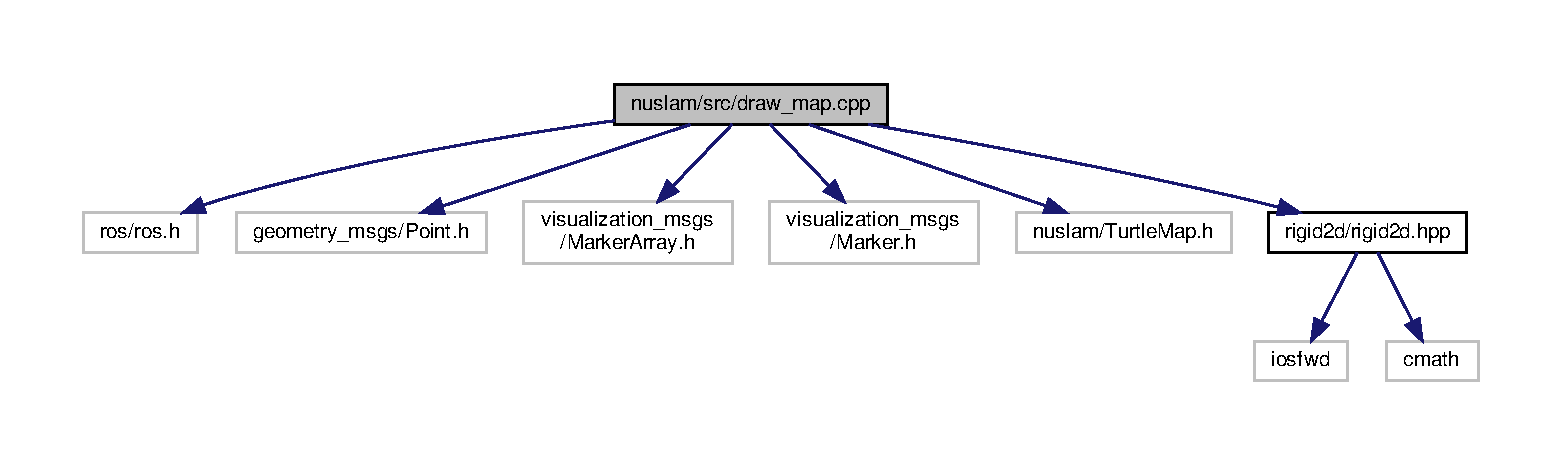
\includegraphics[width=350pt]{df/de5/draw__map_8cpp__incl}
\end{center}
\end{figure}
\subsection*{Functions}
\begin{DoxyCompactItemize}
\item 
\mbox{\Hypertarget{draw__map_8cpp_a382b97f22527718198670efe9d2f07aa}\label{draw__map_8cpp_a382b97f22527718198670efe9d2f07aa}} 
void \hyperlink{draw__map_8cpp_a382b97f22527718198670efe9d2f07aa}{callback\+\_\+landmark\+\_\+data} (nuslam\+::\+Turtle\+Map\+::\+Const\+Ptr data)
\begin{DoxyCompactList}\small\item\em callback fuction for to save the landmark data \end{DoxyCompactList}\item 
\mbox{\Hypertarget{draw__map_8cpp_a3c04138a5bfe5d72780bb7e82a18e627}\label{draw__map_8cpp_a3c04138a5bfe5d72780bb7e82a18e627}} 
int \hyperlink{draw__map_8cpp_a3c04138a5bfe5d72780bb7e82a18e627}{main} (int argc, char $\ast$$\ast$argv)
\begin{DoxyCompactList}\small\item\em main function to create the real\+\_\+waypoints node \end{DoxyCompactList}\end{DoxyCompactItemize}


\subsection{Detailed Description}
This node takes a list of centers and radii to draw the coresponding map. 

P\+A\+R\+A\+M\+E\+T\+E\+RS\+: P\+U\+B\+L\+I\+S\+H\+ES\+: /visualization\+\_\+marker\+\_\+array (visualization\+\_\+msgs\+::\+Marker\+Array) markers S\+U\+B\+S\+C\+R\+I\+B\+ES\+: /landmark\+\_\+data\+: (nuslam/\+Turtle\+Map) a list of centers and radii for cylindrical landmarks S\+E\+R\+I\+V\+C\+ES\+: 
\hypertarget{landmarks_8cpp}{}\section{nuslam/src/landmarks.cpp File Reference}
\label{landmarks_8cpp}\index{nuslam/src/landmarks.\+cpp@{nuslam/src/landmarks.\+cpp}}


This node clusters laser scan data points and fits each cluster to a circular landmark.  


{\ttfamily \#include $<$vector$>$}\newline
{\ttfamily \#include $<$Eigen/\+Dense$>$}\newline
{\ttfamily \#include \char`\"{}ros/ros.\+h\char`\"{}}\newline
{\ttfamily \#include \char`\"{}std\+\_\+msgs/\+Header.\+h\char`\"{}}\newline
{\ttfamily \#include \char`\"{}geometry\+\_\+msgs/\+Point.\+h\char`\"{}}\newline
{\ttfamily \#include \char`\"{}geometry\+\_\+msgs/\+Point32.\+h\char`\"{}}\newline
{\ttfamily \#include \char`\"{}nuslam/\+Turtle\+Map.\+h\char`\"{}}\newline
{\ttfamily \#include \char`\"{}sensor\+\_\+msgs/\+Laser\+Scan.\+h\char`\"{}}\newline
{\ttfamily \#include \char`\"{}sensor\+\_\+msgs/\+Point\+Cloud.\+h\char`\"{}}\newline
{\ttfamily \#include \char`\"{}rigid2d/rigid2d.\+hpp\char`\"{}}\newline
{\ttfamily \#include \char`\"{}nuslam/cylinder\+\_\+detect.\+hpp\char`\"{}}\newline
Include dependency graph for landmarks.\+cpp\+:
\nopagebreak
\begin{figure}[H]
\begin{center}
\leavevmode
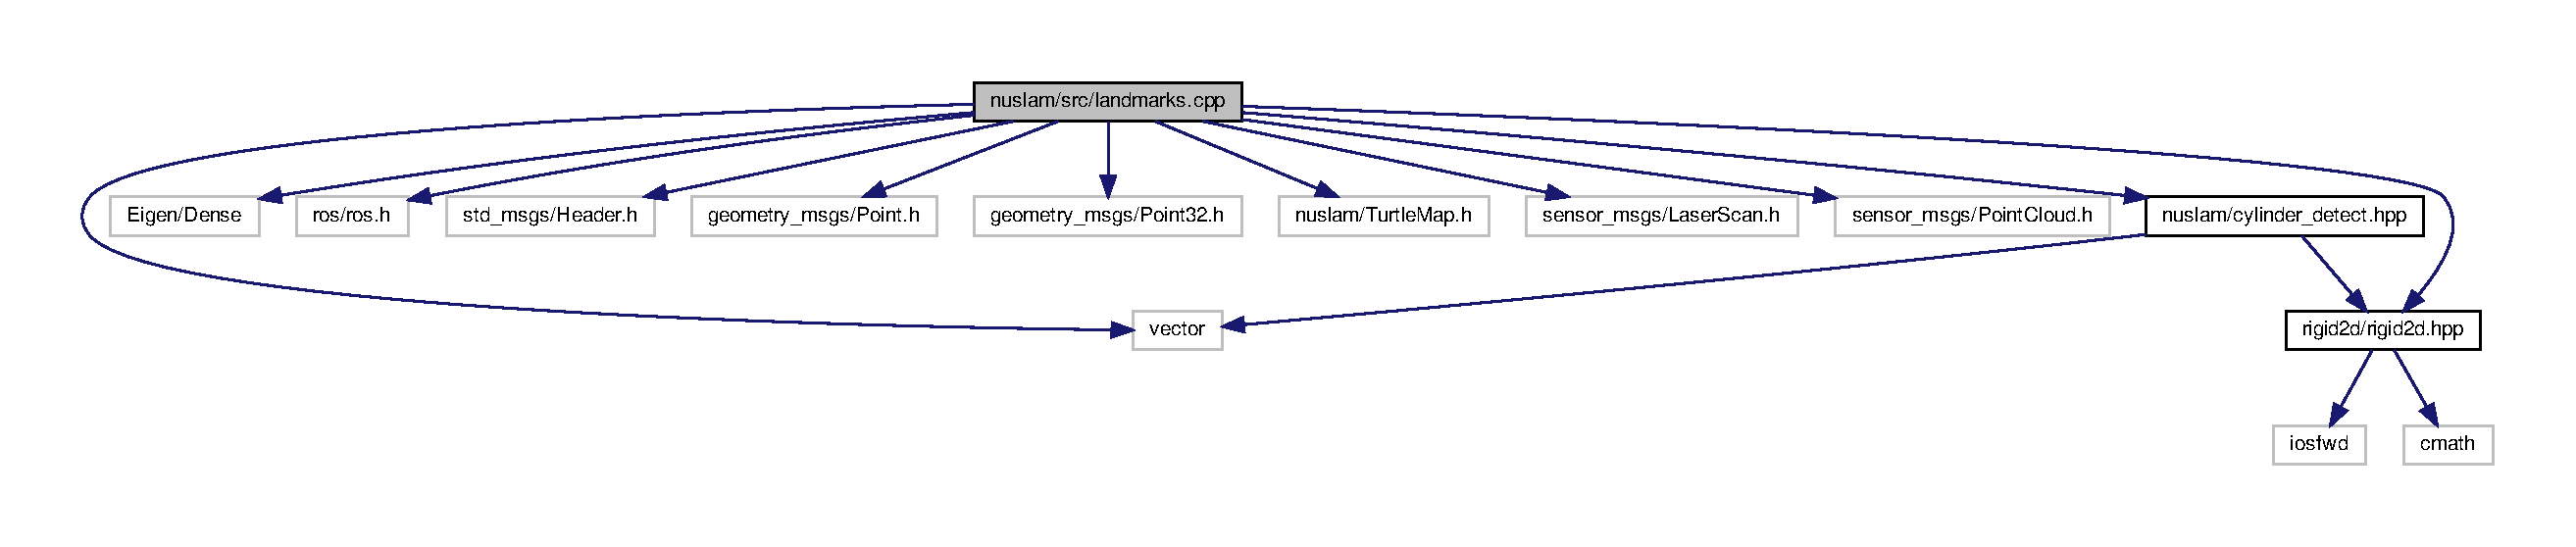
\includegraphics[width=350pt]{d4/d0e/landmarks_8cpp__incl}
\end{center}
\end{figure}
\subsection*{Functions}
\begin{DoxyCompactItemize}
\item 
\hyperlink{structrigid2d_1_1Vector2D}{rigid2d\+::\+Vector2D} \hyperlink{landmarks_8cpp_a9007899199072a8b1e71eeb2635ef9dd}{polar2cart} (double r, double theta)
\begin{DoxyCompactList}\small\item\em converts a point in polar coordinates into cartesian coordinates \end{DoxyCompactList}\item 
\mbox{\Hypertarget{landmarks_8cpp_ab62a3e576fa8343e7c7e299c41ae01f1}\label{landmarks_8cpp_ab62a3e576fa8343e7c7e299c41ae01f1}} 
void \hyperlink{landmarks_8cpp_ab62a3e576fa8343e7c7e299c41ae01f1}{callback\+\_\+robot\+Scan} (sensor\+\_\+msgs\+::\+Laser\+Scan\+::\+Const\+Ptr data)
\begin{DoxyCompactList}\small\item\em Callback function for the sensor subscriber. \end{DoxyCompactList}\item 
\mbox{\Hypertarget{landmarks_8cpp_a3c04138a5bfe5d72780bb7e82a18e627}\label{landmarks_8cpp_a3c04138a5bfe5d72780bb7e82a18e627}} 
int \hyperlink{landmarks_8cpp_a3c04138a5bfe5d72780bb7e82a18e627}{main} (int argc, char $\ast$$\ast$argv)
\begin{DoxyCompactList}\small\item\em main function to create the real\+\_\+waypoints node \end{DoxyCompactList}\end{DoxyCompactItemize}


\subsection{Detailed Description}
This node clusters laser scan data points and fits each cluster to a circular landmark. 

P\+A\+R\+A\+M\+E\+T\+E\+RS\+: distance\+\_\+threshold\+: (double) Threshold to determine if a point is in a cluster radius\+\_\+threshold\+: (double) Threshold to determine if a cirlce fit is valid for an obstacle frame\+\_\+id\+: (string) The frame the Laser scan data is relative to P\+U\+B\+L\+I\+S\+H\+ES\+: /landmark\+\_\+data\+: (nuslam/\+Turtle\+Map) a list of centers and radii for cylindrical landmarks S\+U\+B\+S\+C\+R\+I\+B\+ES\+: /scan\+: (sensor\+\_\+msgs/\+Laser\+Scan) the raw laser data from the turtlebot S\+E\+R\+I\+V\+C\+ES\+: 

\subsection{Function Documentation}
\mbox{\Hypertarget{landmarks_8cpp_a9007899199072a8b1e71eeb2635ef9dd}\label{landmarks_8cpp_a9007899199072a8b1e71eeb2635ef9dd}} 
\index{landmarks.\+cpp@{landmarks.\+cpp}!polar2cart@{polar2cart}}
\index{polar2cart@{polar2cart}!landmarks.\+cpp@{landmarks.\+cpp}}
\subsubsection{\texorpdfstring{polar2cart()}{polar2cart()}}
{\footnotesize\ttfamily \hyperlink{structrigid2d_1_1Vector2D}{rigid2d\+::\+Vector2D} polar2cart (\begin{DoxyParamCaption}\item[{double}]{r,  }\item[{double}]{theta }\end{DoxyParamCaption})}



converts a point in polar coordinates into cartesian coordinates 


\begin{DoxyParams}{Parameters}
{\em r} & the distange to the point \\
\hline
{\em theta} & the angle to the point \\
\hline
\end{DoxyParams}
\begin{DoxyReturn}{Returns}
(\hyperlink{structrigid2d_1_1Vector2D}{rigid2d\+::\+Vector2D}) x,y coordinates of the point 
\end{DoxyReturn}

\hypertarget{slam_8cpp}{}\section{nuslam/src/slam.cpp File Reference}
\label{slam_8cpp}\index{nuslam/src/slam.\+cpp@{nuslam/src/slam.\+cpp}}


This node publishes an estimate of the robot state using E\+KF S\+L\+AM.  


{\ttfamily \#include $<$iostream$>$}\newline
{\ttfamily \#include $<$ros/ros.\+h$>$}\newline
{\ttfamily \#include $<$tf2\+\_\+ros/transform\+\_\+broadcaster.\+h$>$}\newline
{\ttfamily \#include $<$tf2/\+Linear\+Math/\+Quaternion.\+h$>$}\newline
{\ttfamily \#include $<$tf2\+\_\+geometry\+\_\+msgs/tf2\+\_\+geometry\+\_\+msgs.\+h$>$}\newline
{\ttfamily \#include $<$geometry\+\_\+msgs/\+Transform\+Stamped.\+h$>$}\newline
{\ttfamily \#include $<$geometry\+\_\+msgs/\+Quaternion.\+h$>$}\newline
{\ttfamily \#include $<$nav\+\_\+msgs/\+Odometry.\+h$>$}\newline
{\ttfamily \#include $<$nav\+\_\+msgs/\+Path.\+h$>$}\newline
{\ttfamily \#include $<$sensor\+\_\+msgs/\+Joint\+State.\+h$>$}\newline
{\ttfamily \#include \char`\"{}nuslam/\+Turtle\+Map.\+h\char`\"{}}\newline
{\ttfamily \#include \char`\"{}rigid2d/\+Set\+Pose.\+h\char`\"{}}\newline
{\ttfamily \#include \char`\"{}rigid2d/rigid2d.\+hpp\char`\"{}}\newline
{\ttfamily \#include \char`\"{}rigid2d/diff\+\_\+drive.\+hpp\char`\"{}}\newline
{\ttfamily \#include \char`\"{}nuslam/ekf\+\_\+slam.\+hpp\char`\"{}}\newline
Include dependency graph for slam.\+cpp\+:\nopagebreak
\begin{figure}[H]
\begin{center}
\leavevmode
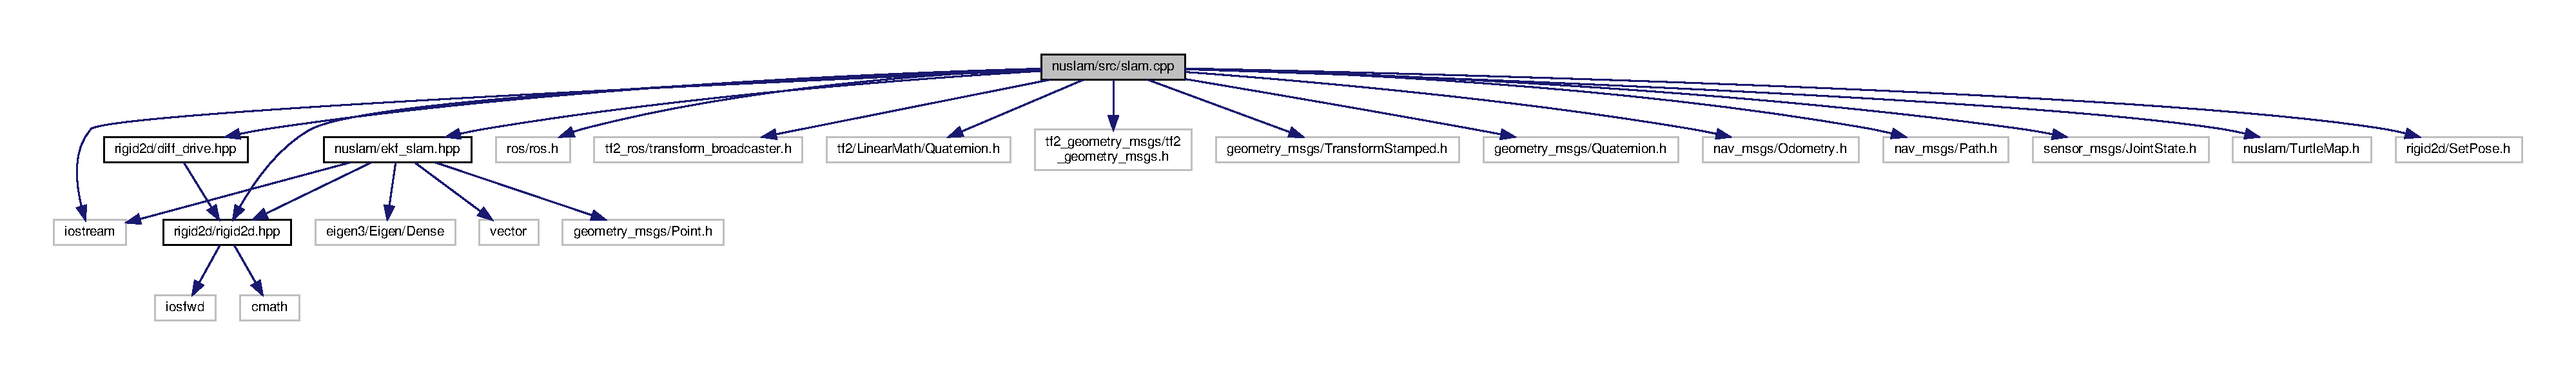
\includegraphics[width=350pt]{d2/d57/slam_8cpp__incl}
\end{center}
\end{figure}
\subsection*{Functions}
\begin{DoxyCompactItemize}
\item 
int \hyperlink{slam_8cpp_ad248270d37c5224dcb705be8b925ff29}{find\+Joint\+Index} (std\+::vector$<$ std\+::string $>$ joints, std\+::string target)
\begin{DoxyCompactList}\small\item\em Use to search through the all joint names and return the index of the desired joint. \end{DoxyCompactList}\item 
\mbox{\Hypertarget{slam_8cpp_a32393f00b4e0f87fc20fd049f9f29e13}\label{slam_8cpp_a32393f00b4e0f87fc20fd049f9f29e13}} 
void \hyperlink{slam_8cpp_a32393f00b4e0f87fc20fd049f9f29e13}{callback\+\_\+joints} (const sensor\+\_\+msgs\+::\+Joint\+State\+::\+Const\+Ptr data)
\begin{DoxyCompactList}\small\item\em Callback for the joint state subscriber. \end{DoxyCompactList}\item 
\mbox{\Hypertarget{slam_8cpp_af118ce6bdc73b978a440f3f2b69e32e4}\label{slam_8cpp_af118ce6bdc73b978a440f3f2b69e32e4}} 
void \hyperlink{slam_8cpp_af118ce6bdc73b978a440f3f2b69e32e4}{callback\+\_\+landmarks} (const nuslam\+::\+Turtle\+Map\+::\+Const\+Ptr data)
\begin{DoxyCompactList}\small\item\em Callback for the landmark data. \end{DoxyCompactList}\item 
\mbox{\Hypertarget{slam_8cpp_a3c04138a5bfe5d72780bb7e82a18e627}\label{slam_8cpp_a3c04138a5bfe5d72780bb7e82a18e627}} 
int \hyperlink{slam_8cpp_a3c04138a5bfe5d72780bb7e82a18e627}{main} (int argc, char $\ast$$\ast$argv)
\begin{DoxyCompactList}\small\item\em Main function for the odometer node. \end{DoxyCompactList}\end{DoxyCompactItemize}


\subsection{Detailed Description}
This node publishes an estimate of the robot state using E\+KF S\+L\+AM. 

P\+A\+R\+A\+M\+E\+T\+E\+RS\+: odom\+\_\+frame\+\_\+id (std\+::string) the name of the odometer frame base\+\_\+frame\+\_\+id (std\+::string) the name of the base frame left\+\_\+wheel\+\_\+joint (std\+::string) the name of the left wheel joint right\+\_\+wheel\+\_\+joint (std\+::string) the name of the right wheel joint wheel\+\_\+base (double) the distance between the two wheels of the diff drive robot wheel\+\_\+radius (double) the radius of the wheels frequency (double) the frequency to publish joint states at num\+\_\+landmarks (int) the number of landmarks allowed in the state vector map\+\_\+frame\+\_\+id (std\+::string) the name of the map frame P\+U\+B\+L\+I\+S\+H\+ES\+: /odom\+\_\+path (nav\+\_\+msgs/\+Path)\+: The path of the robot following purely odometry /slam\+\_\+path (nav\+\_\+msgs/\+Path)\+: The path of the robot following slam estimate /slam\+\_\+landmark\+\_\+data (nuslam/\+Turtle\+Map)\+: landmark state estimate from slam S\+U\+B\+S\+C\+R\+I\+B\+ES\+: /joint\+\_\+states (sensor\+\_\+msgs/\+Joint\+State)\+: Retrieves the calculated wheel velocities and change in wheel position /landmark\+\_\+data (nuslam/\+Turtle\+Map)\+: landmark position and size information 

\subsection{Function Documentation}
\mbox{\Hypertarget{slam_8cpp_ad248270d37c5224dcb705be8b925ff29}\label{slam_8cpp_ad248270d37c5224dcb705be8b925ff29}} 
\index{slam.\+cpp@{slam.\+cpp}!find\+Joint\+Index@{find\+Joint\+Index}}
\index{find\+Joint\+Index@{find\+Joint\+Index}!slam.\+cpp@{slam.\+cpp}}
\subsubsection{\texorpdfstring{find\+Joint\+Index()}{findJointIndex()}}
{\footnotesize\ttfamily int find\+Joint\+Index (\begin{DoxyParamCaption}\item[{std\+::vector$<$ std\+::string $>$}]{joints,  }\item[{std\+::string}]{target }\end{DoxyParamCaption})}



Use to search through the all joint names and return the index of the desired joint. 


\begin{DoxyParams}{Parameters}
{\em joints} & -\/ a vector of all the joint names \\
\hline
{\em target} & -\/ the desire joint name to find \\
\hline
\end{DoxyParams}
\begin{DoxyReturn}{Returns}
the index of the desired joint name 
\end{DoxyReturn}

\hypertarget{test__landmarks_8cpp}{}\section{nuslam/test/test\+\_\+landmarks.cpp File Reference}
\label{test__landmarks_8cpp}\index{nuslam/test/test\+\_\+landmarks.\+cpp@{nuslam/test/test\+\_\+landmarks.\+cpp}}


This node tests the landmark node circle fitting functions.  


{\ttfamily \#include $<$gtest/gtest.\+h$>$}\newline
{\ttfamily \#include $<$sstream$>$}\newline
{\ttfamily \#include $<$iostream$>$}\newline
{\ttfamily \#include $<$vector$>$}\newline
{\ttfamily \#include \char`\"{}rigid2d/rigid2d.\+hpp\char`\"{}}\newline
{\ttfamily \#include \char`\"{}nuslam/cylinder\+\_\+detect.\+hpp\char`\"{}}\newline
Include dependency graph for test\+\_\+landmarks.\+cpp\+:\nopagebreak
\begin{figure}[H]
\begin{center}
\leavevmode
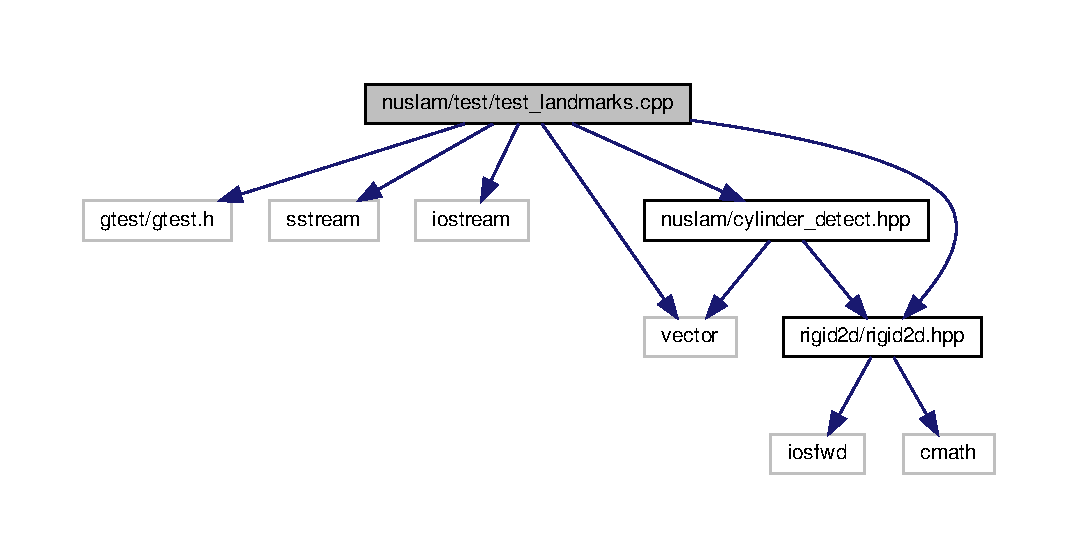
\includegraphics[width=350pt]{d7/d4e/test__landmarks_8cpp__incl}
\end{center}
\end{figure}
\subsection*{Functions}
\begin{DoxyCompactItemize}
\item 
\mbox{\Hypertarget{test__landmarks_8cpp_a384522a7bfc39e94d18b53b8786bfa1e}\label{test__landmarks_8cpp_a384522a7bfc39e94d18b53b8786bfa1e}} 
{\bfseries T\+E\+ST} (Landmark, Circle\+Test1)
\item 
\mbox{\Hypertarget{test__landmarks_8cpp_aa9c3f3945309c0d42ecf3816d5a3d199}\label{test__landmarks_8cpp_aa9c3f3945309c0d42ecf3816d5a3d199}} 
{\bfseries T\+E\+ST} (Landmark, Circle\+Test2)
\end{DoxyCompactItemize}


\subsection{Detailed Description}
This node tests the landmark node circle fitting functions. 


\hypertarget{real__waypoints_8cpp}{}\section{nuturtle\+\_\+robot/src/real\+\_\+waypoints.cpp File Reference}
\label{real__waypoints_8cpp}\index{nuturtle\+\_\+robot/src/real\+\_\+waypoints.\+cpp@{nuturtle\+\_\+robot/src/real\+\_\+waypoints.\+cpp}}


This node publishes a twist to drive the turtlebot along a path of waypoints.  


{\ttfamily \#include $<$ros/ros.\+h$>$}\newline
{\ttfamily \#include $<$iostream$>$}\newline
{\ttfamily \#include $<$tf2/\+Linear\+Math/\+Quaternion.\+h$>$}\newline
{\ttfamily \#include $<$tf2\+\_\+geometry\+\_\+msgs/tf2\+\_\+geometry\+\_\+msgs.\+h$>$}\newline
{\ttfamily \#include \char`\"{}rigid2d/rigid2d.\+hpp\char`\"{}}\newline
{\ttfamily \#include \char`\"{}rigid2d/waypoints.\+hpp\char`\"{}}\newline
{\ttfamily \#include $<$geometry\+\_\+msgs/\+Twist.\+h$>$}\newline
{\ttfamily \#include $<$geometry\+\_\+msgs/\+Quaternion.\+h$>$}\newline
{\ttfamily \#include $<$nav\+\_\+msgs/\+Odometry.\+h$>$}\newline
{\ttfamily \#include $<$std\+\_\+srvs/\+Empty.\+h$>$}\newline
{\ttfamily \#include \char`\"{}rigid2d/\+Set\+Pose.\+h\char`\"{}}\newline
{\ttfamily \#include \char`\"{}rigid2d/\+Pose.\+h\char`\"{}}\newline
{\ttfamily \#include $<$visualization\+\_\+msgs/\+Marker.\+h$>$}\newline
Include dependency graph for real\+\_\+waypoints.\+cpp\+:
\nopagebreak
\begin{figure}[H]
\begin{center}
\leavevmode
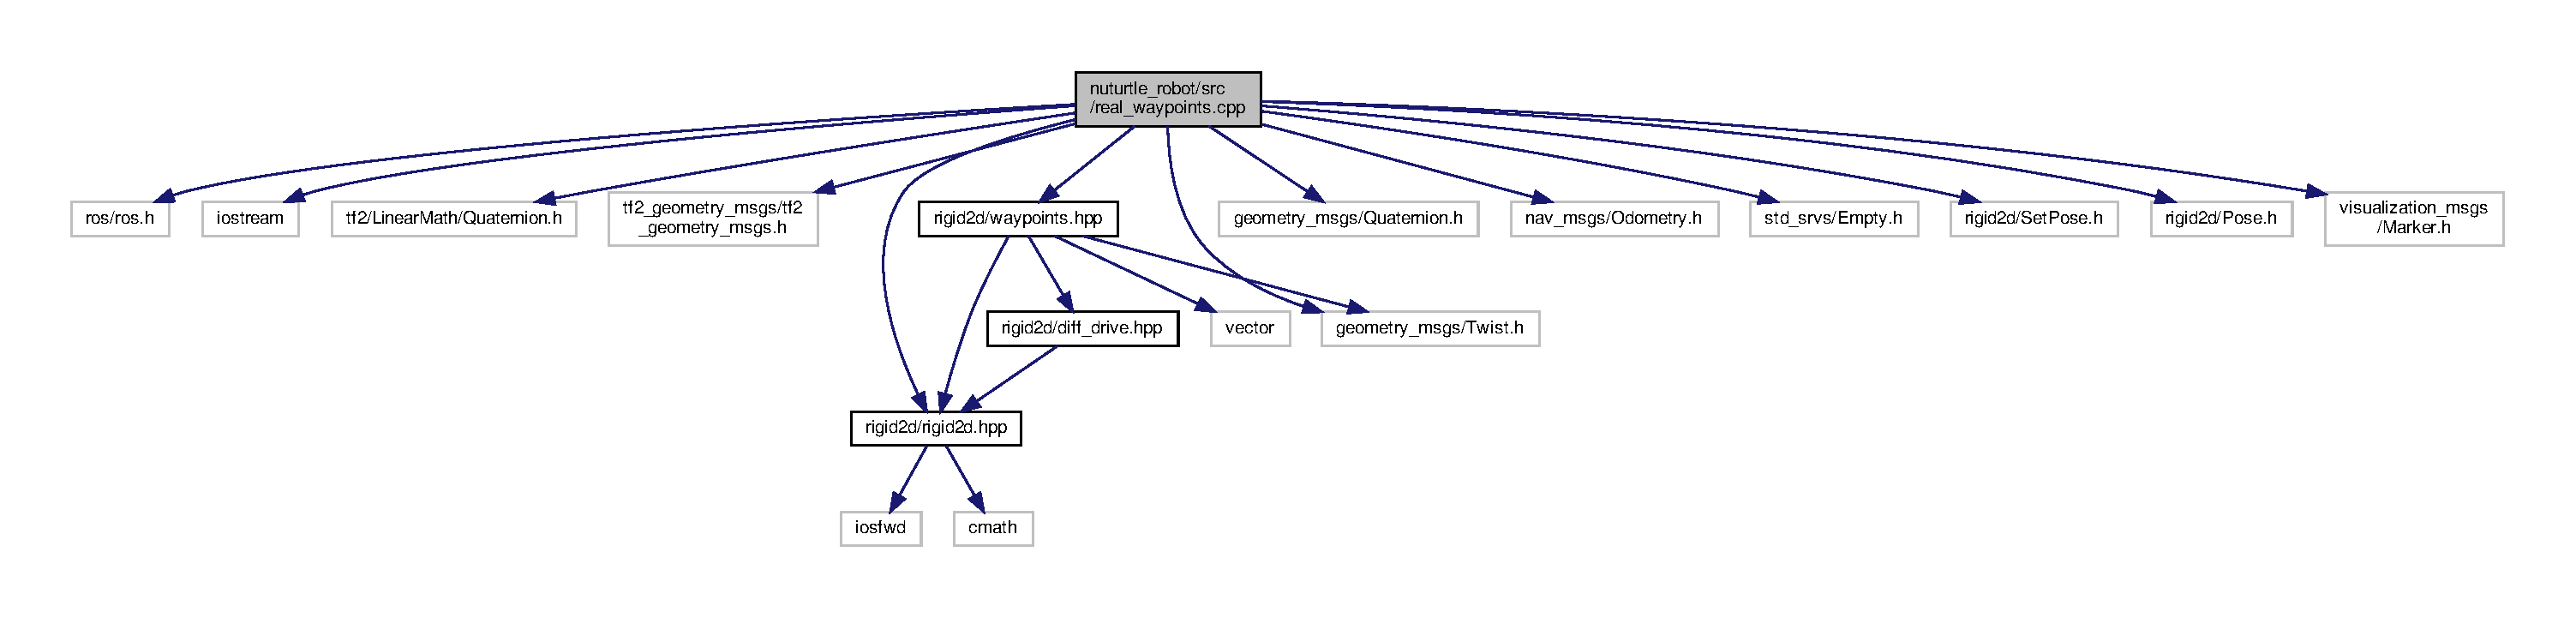
\includegraphics[width=350pt]{dc/d52/real__waypoints_8cpp__incl}
\end{center}
\end{figure}
\subsection*{Functions}
\begin{DoxyCompactItemize}
\item 
\mbox{\Hypertarget{real__waypoints_8cpp_a6101e6c32b9cbe3586175efc2a0096eb}\label{real__waypoints_8cpp_a6101e6c32b9cbe3586175efc2a0096eb}} 
bool \hyperlink{real__waypoints_8cpp_a6101e6c32b9cbe3586175efc2a0096eb}{callback\+\_\+start} (std\+\_\+srvs\+::\+Empty\+::\+Request \&, std\+\_\+srvs\+::\+Empty\+::\+Response \&)
\begin{DoxyCompactList}\small\item\em Callback for the start service \end{DoxyCompactList}\item 
\mbox{\Hypertarget{real__waypoints_8cpp_ae6f5d827466617c084abe7ac286d4f27}\label{real__waypoints_8cpp_ae6f5d827466617c084abe7ac286d4f27}} 
void \hyperlink{real__waypoints_8cpp_ae6f5d827466617c084abe7ac286d4f27}{callback\+\_\+pose} (nav\+\_\+msgs\+::\+Odometry\+::\+Const\+Ptr odom)
\begin{DoxyCompactList}\small\item\em Callback for the odom subscriber \end{DoxyCompactList}\item 
\mbox{\Hypertarget{real__waypoints_8cpp_a8bc0a8cc07be82fba19164d8a67bcb66}\label{real__waypoints_8cpp_a8bc0a8cc07be82fba19164d8a67bcb66}} 
bool \hyperlink{real__waypoints_8cpp_a8bc0a8cc07be82fba19164d8a67bcb66}{callback\+\_\+stop} (std\+\_\+srvs\+::\+Empty\+::\+Request \&, std\+\_\+srvs\+::\+Empty\+::\+Response \&)
\begin{DoxyCompactList}\small\item\em Callback for the stop service \end{DoxyCompactList}\item 
\mbox{\Hypertarget{real__waypoints_8cpp_a3c04138a5bfe5d72780bb7e82a18e627}\label{real__waypoints_8cpp_a3c04138a5bfe5d72780bb7e82a18e627}} 
int \hyperlink{real__waypoints_8cpp_a3c04138a5bfe5d72780bb7e82a18e627}{main} (int argc, char $\ast$$\ast$argv)
\begin{DoxyCompactList}\small\item\em main function to create the real\+\_\+waypoints node \end{DoxyCompactList}\end{DoxyCompactItemize}
\subsection*{Variables}
\begin{DoxyCompactItemize}
\item 
\mbox{\Hypertarget{real__waypoints_8cpp_af884c9d7e4937faf15d46131d87c8f93}\label{real__waypoints_8cpp_af884c9d7e4937faf15d46131d87c8f93}} 
ros\+::\+Publisher {\bfseries marker\+\_\+pub}
\end{DoxyCompactItemize}


\subsection{Detailed Description}
This node publishes a twist to drive the turtlebot along a path of waypoints. 

P\+A\+R\+A\+M\+E\+T\+E\+RS\+: frac\+\_\+val\+: (double) proportion of max speed to use avel\+\_\+lim\+: (double) max robot angular velocity tvel\+\_\+lim\+: (double) max robot linear velocity frequency\+: (int) frequency to publish at waypoint\+\_\+x\+: (double) A list of the x coordinates for a series of waypoints waypoint\+\_\+y\+: (double) A list of the y coordinates for a series of waypoints P\+U\+B\+L\+I\+S\+H\+ES\+: /cmd\+\_\+vel\+: (geometry\+\_\+msgs/\+Twist) the twist command S\+U\+B\+S\+C\+R\+I\+B\+ES\+: /odom\+: (nav\+\_\+msgs/\+Odometry) the current estimated pose of the robot S\+E\+R\+I\+V\+C\+ES\+: /start\+: (std\+\_\+srvs/\+Empty) Starts the movement of the robot /stop\+: (std\+\_\+srvs/\+Empty) Stops the movement of the robot 
\hypertarget{rotation_8cpp}{}\section{nuturtle\+\_\+robot/src/rotation.cpp File Reference}
\label{rotation_8cpp}\index{nuturtle\+\_\+robot/src/rotation.\+cpp@{nuturtle\+\_\+robot/src/rotation.\+cpp}}


This node interfaces between a main computer and the raspberri pi on the turtlebot.  


{\ttfamily \#include $<$ros/ros.\+h$>$}\newline
{\ttfamily \#include \char`\"{}rigid2d/rigid2d.\+hpp\char`\"{}}\newline
{\ttfamily \#include $<$geometry\+\_\+msgs/\+Twist.\+h$>$}\newline
{\ttfamily \#include $<$std\+\_\+srvs/\+Set\+Bool.\+h$>$}\newline
{\ttfamily \#include \char`\"{}rigid2d/\+Set\+Pose.\+h\char`\"{}}\newline
{\ttfamily \#include \char`\"{}rigid2d/\+Pose.\+h\char`\"{}}\newline
Include dependency graph for rotation.\+cpp\+:
\nopagebreak
\begin{figure}[H]
\begin{center}
\leavevmode
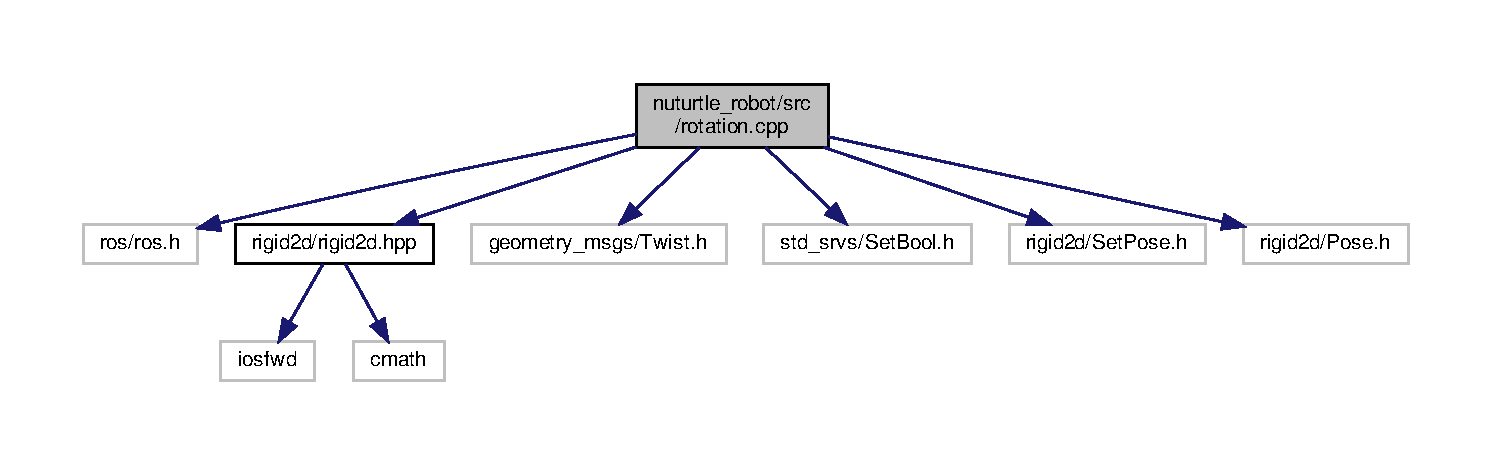
\includegraphics[width=350pt]{dc/df1/rotation_8cpp__incl}
\end{center}
\end{figure}
\subsection*{Functions}
\begin{DoxyCompactItemize}
\item 
bool \hyperlink{rotation_8cpp_a8a003764bae77bc3a8d005a76365ce0b}{callback\+\_\+start} (std\+\_\+srvs\+::\+Set\+Bool\+::\+Request \&req, std\+\_\+srvs\+::\+Set\+Bool\+::\+Response \&)
\begin{DoxyCompactList}\small\item\em Callback for start service. \end{DoxyCompactList}\item 
void \hyperlink{rotation_8cpp_a6f56faf21488465a1fc832f74a795952}{callback\+\_\+timer} (const ros\+::\+Timer\+Event \&)
\begin{DoxyCompactList}\small\item\em Callback for Timer. \end{DoxyCompactList}\item 
\mbox{\Hypertarget{rotation_8cpp_a3c04138a5bfe5d72780bb7e82a18e627}\label{rotation_8cpp_a3c04138a5bfe5d72780bb7e82a18e627}} 
int \hyperlink{rotation_8cpp_a3c04138a5bfe5d72780bb7e82a18e627}{main} (int argc, char $\ast$$\ast$argv)
\begin{DoxyCompactList}\small\item\em main function to create the rotation node \end{DoxyCompactList}\end{DoxyCompactItemize}


\subsection{Detailed Description}
This node interfaces between a main computer and the raspberri pi on the turtlebot. 

P\+A\+R\+A\+M\+E\+T\+E\+RS\+: /rotation/frac\+\_\+val\+: proportion of max speed to use /avel\+\_\+lim\+: max robot angular velocity P\+U\+B\+L\+I\+S\+H\+ES\+: /cmd\+\_\+vel (geometry\+\_\+msgs/\+Twist)\+: the twist command S\+E\+R\+I\+V\+C\+ES\+: /start (std\+\_\+srvs/\+Set\+Bool)\+: Starts the movement of the robot given an initial direction. 0 is C\+C\+W/\+Forwards, 1 is C\+W/\+Backwards 

\subsection{Function Documentation}
\mbox{\Hypertarget{rotation_8cpp_a8a003764bae77bc3a8d005a76365ce0b}\label{rotation_8cpp_a8a003764bae77bc3a8d005a76365ce0b}} 
\index{rotation.\+cpp@{rotation.\+cpp}!callback\+\_\+start@{callback\+\_\+start}}
\index{callback\+\_\+start@{callback\+\_\+start}!rotation.\+cpp@{rotation.\+cpp}}
\subsubsection{\texorpdfstring{callback\+\_\+start()}{callback\_start()}}
{\footnotesize\ttfamily bool callback\+\_\+start (\begin{DoxyParamCaption}\item[{std\+\_\+srvs\+::\+Set\+Bool\+::\+Request \&}]{req,  }\item[{std\+\_\+srvs\+::\+Set\+Bool\+::\+Response \&}]{ }\end{DoxyParamCaption})}



Callback for start service. 

\begin{DoxyReturn}{Returns}
1 for success 
\end{DoxyReturn}
\mbox{\Hypertarget{rotation_8cpp_a6f56faf21488465a1fc832f74a795952}\label{rotation_8cpp_a6f56faf21488465a1fc832f74a795952}} 
\index{rotation.\+cpp@{rotation.\+cpp}!callback\+\_\+timer@{callback\+\_\+timer}}
\index{callback\+\_\+timer@{callback\+\_\+timer}!rotation.\+cpp@{rotation.\+cpp}}
\subsubsection{\texorpdfstring{callback\+\_\+timer()}{callback\_timer()}}
{\footnotesize\ttfamily void callback\+\_\+timer (\begin{DoxyParamCaption}\item[{const ros\+::\+Timer\+Event \&}]{ }\end{DoxyParamCaption})}



Callback for Timer. 

\begin{DoxyReturn}{Returns}
1 for success 
\end{DoxyReturn}

\hypertarget{test__turtle__interface_8cpp}{}\section{nuturtle\+\_\+robot/src/test/test\+\_\+turtle\+\_\+interface.cpp File Reference}
\label{test__turtle__interface_8cpp}\index{nuturtle\+\_\+robot/src/test/test\+\_\+turtle\+\_\+interface.\+cpp@{nuturtle\+\_\+robot/src/test/test\+\_\+turtle\+\_\+interface.\+cpp}}


This node tests the turtle interface node.  


{\ttfamily \#include $<$gtest/gtest.\+h$>$}\newline
{\ttfamily \#include $<$sstream$>$}\newline
{\ttfamily \#include $<$ros/ros.\+h$>$}\newline
{\ttfamily \#include \char`\"{}rigid2d/rigid2d.\+hpp\char`\"{}}\newline
{\ttfamily \#include \char`\"{}geometry\+\_\+msgs/\+Twist.\+h\char`\"{}}\newline
{\ttfamily \#include \char`\"{}nuturtlebot/\+Wheel\+Commands.\+h\char`\"{}}\newline
{\ttfamily \#include \char`\"{}nuturtlebot/\+Sensor\+Data.\+h\char`\"{}}\newline
{\ttfamily \#include \char`\"{}sensor\+\_\+msgs/\+Joint\+State.\+h\char`\"{}}\newline
Include dependency graph for test\+\_\+turtle\+\_\+interface.\+cpp\+:\nopagebreak
\begin{figure}[H]
\begin{center}
\leavevmode
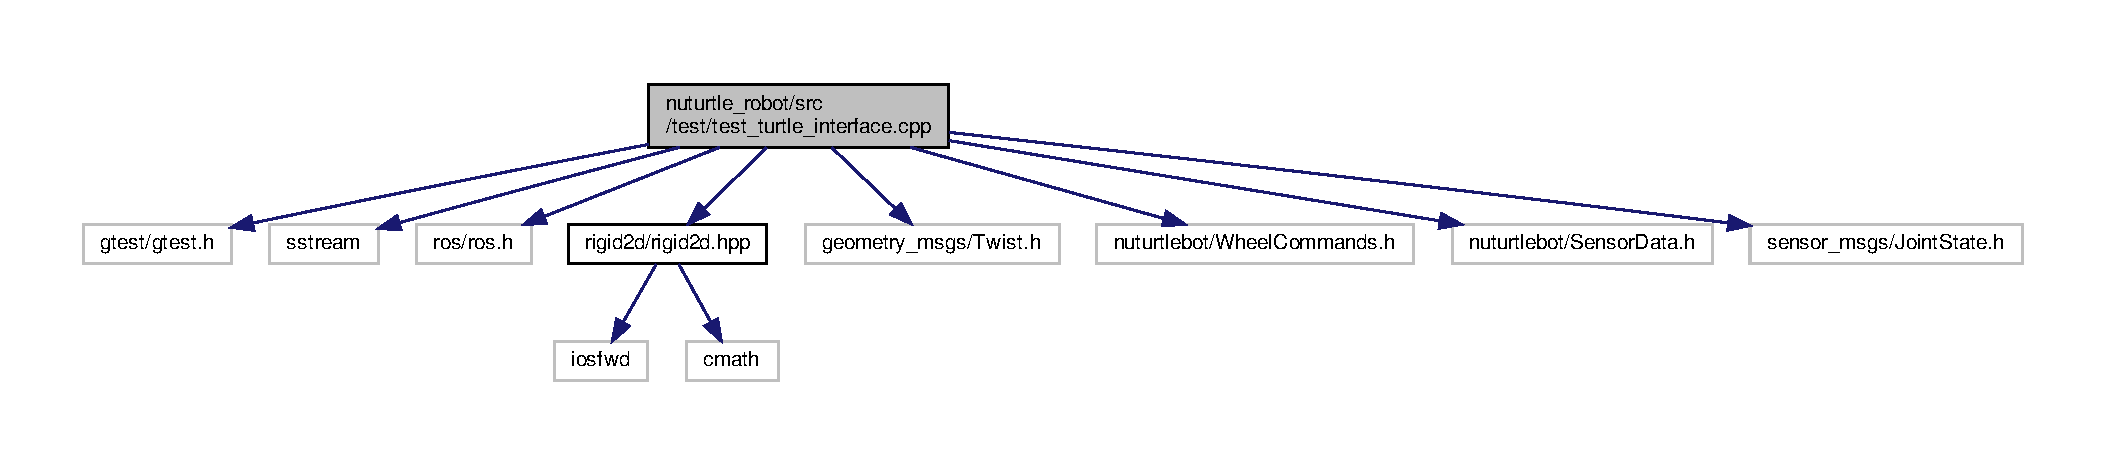
\includegraphics[width=350pt]{d0/df1/test__turtle__interface_8cpp__incl}
\end{center}
\end{figure}
\subsection*{Functions}
\begin{DoxyCompactItemize}
\item 
\mbox{\Hypertarget{test__turtle__interface_8cpp_aba35a82eceda5d601d138e18c85739c4}\label{test__turtle__interface_8cpp_aba35a82eceda5d601d138e18c85739c4}} 
void \hyperlink{test__turtle__interface_8cpp_aba35a82eceda5d601d138e18c85739c4}{callback\+\_\+wheels} (nuturtlebot\+::\+Wheel\+Commands\+::\+Const\+Ptr data)
\begin{DoxyCompactList}\small\item\em Callback for wheel\+\_\+cmd subscriber \end{DoxyCompactList}\item 
\mbox{\Hypertarget{test__turtle__interface_8cpp_a04d67c3fcfa3f2187242f4f77997ab41}\label{test__turtle__interface_8cpp_a04d67c3fcfa3f2187242f4f77997ab41}} 
void \hyperlink{test__turtle__interface_8cpp_a04d67c3fcfa3f2187242f4f77997ab41}{callback\+\_\+joints} (sensor\+\_\+msgs\+::\+Joint\+State\+::\+Const\+Ptr data)
\begin{DoxyCompactList}\small\item\em Callback for joint\+\_\+states subscriber \end{DoxyCompactList}\item 
\mbox{\Hypertarget{test__turtle__interface_8cpp_a171da9d53bcf1e807cacb1669fdf90a2}\label{test__turtle__interface_8cpp_a171da9d53bcf1e807cacb1669fdf90a2}} 
{\bfseries T\+E\+ST} (Turtle\+Interface, Trans\+Only)
\item 
\mbox{\Hypertarget{test__turtle__interface_8cpp_adeeeef210e8b88091ff2bcbf5029ce13}\label{test__turtle__interface_8cpp_adeeeef210e8b88091ff2bcbf5029ce13}} 
{\bfseries T\+E\+ST} (Turtle\+Interface, Rot\+Only)
\item 
\mbox{\Hypertarget{test__turtle__interface_8cpp_a9255d0ecfb79606f015d9d6a8a379bcd}\label{test__turtle__interface_8cpp_a9255d0ecfb79606f015d9d6a8a379bcd}} 
{\bfseries T\+E\+ST} (Turtle\+Interface, Rot\+And\+Trans)
\item 
\mbox{\Hypertarget{test__turtle__interface_8cpp_a95b1341f9409103ab6305ef4b678facd}\label{test__turtle__interface_8cpp_a95b1341f9409103ab6305ef4b678facd}} 
{\bfseries T\+E\+ST} (Turtle\+Interface, Valid\+Encs)
\item 
\mbox{\Hypertarget{test__turtle__interface_8cpp_a3c04138a5bfe5d72780bb7e82a18e627}\label{test__turtle__interface_8cpp_a3c04138a5bfe5d72780bb7e82a18e627}} 
int {\bfseries main} (int argc, char $\ast$$\ast$argv)
\end{DoxyCompactItemize}


\subsection{Detailed Description}
This node tests the turtle interface node. 

P\+U\+B\+L\+I\+S\+H\+ES\+: /cmd\+\_\+vel (geometry\+\_\+msgs/\+Twist)\+: the twist command from the turtlesim package /sensor\+\_\+data (nuturtlebot/\+Sensor\+Data)\+: retrives sensor info from the turtlebot S\+U\+B\+S\+C\+R\+I\+B\+ES\+: /wheel\+\_\+cmd (nutrutlebot/\+Wheel\+Commands)\+: a command to control the motors on the turtlebot /joint\+\_\+states (sensor\+\_\+msgs/\+Joint\+State)\+: the wheel position and velocities of the turtlebot 
\hypertarget{turtle__interface_8cpp}{}\section{nuturtle\+\_\+robot/src/turtle\+\_\+interface.cpp File Reference}
\label{turtle__interface_8cpp}\index{nuturtle\+\_\+robot/src/turtle\+\_\+interface.\+cpp@{nuturtle\+\_\+robot/src/turtle\+\_\+interface.\+cpp}}


This node interfaces between a main computer and the raspberri pi on the turtlebot.  


{\ttfamily \#include $<$iostream$>$}\newline
{\ttfamily \#include $<$ros/ros.\+h$>$}\newline
{\ttfamily \#include $<$geometry\+\_\+msgs/\+Twist.\+h$>$}\newline
{\ttfamily \#include $<$sensor\+\_\+msgs/\+Joint\+State.\+h$>$}\newline
{\ttfamily \#include \char`\"{}nuturtlebot/\+Sensor\+Data.\+h\char`\"{}}\newline
{\ttfamily \#include \char`\"{}nuturtlebot/\+Wheel\+Commands.\+h\char`\"{}}\newline
{\ttfamily \#include \char`\"{}rigid2d/diff\+\_\+drive.\+hpp\char`\"{}}\newline
{\ttfamily \#include \char`\"{}rigid2d/waypoints.\+hpp\char`\"{}}\newline
Include dependency graph for turtle\+\_\+interface.\+cpp\+:\nopagebreak
\begin{figure}[H]
\begin{center}
\leavevmode
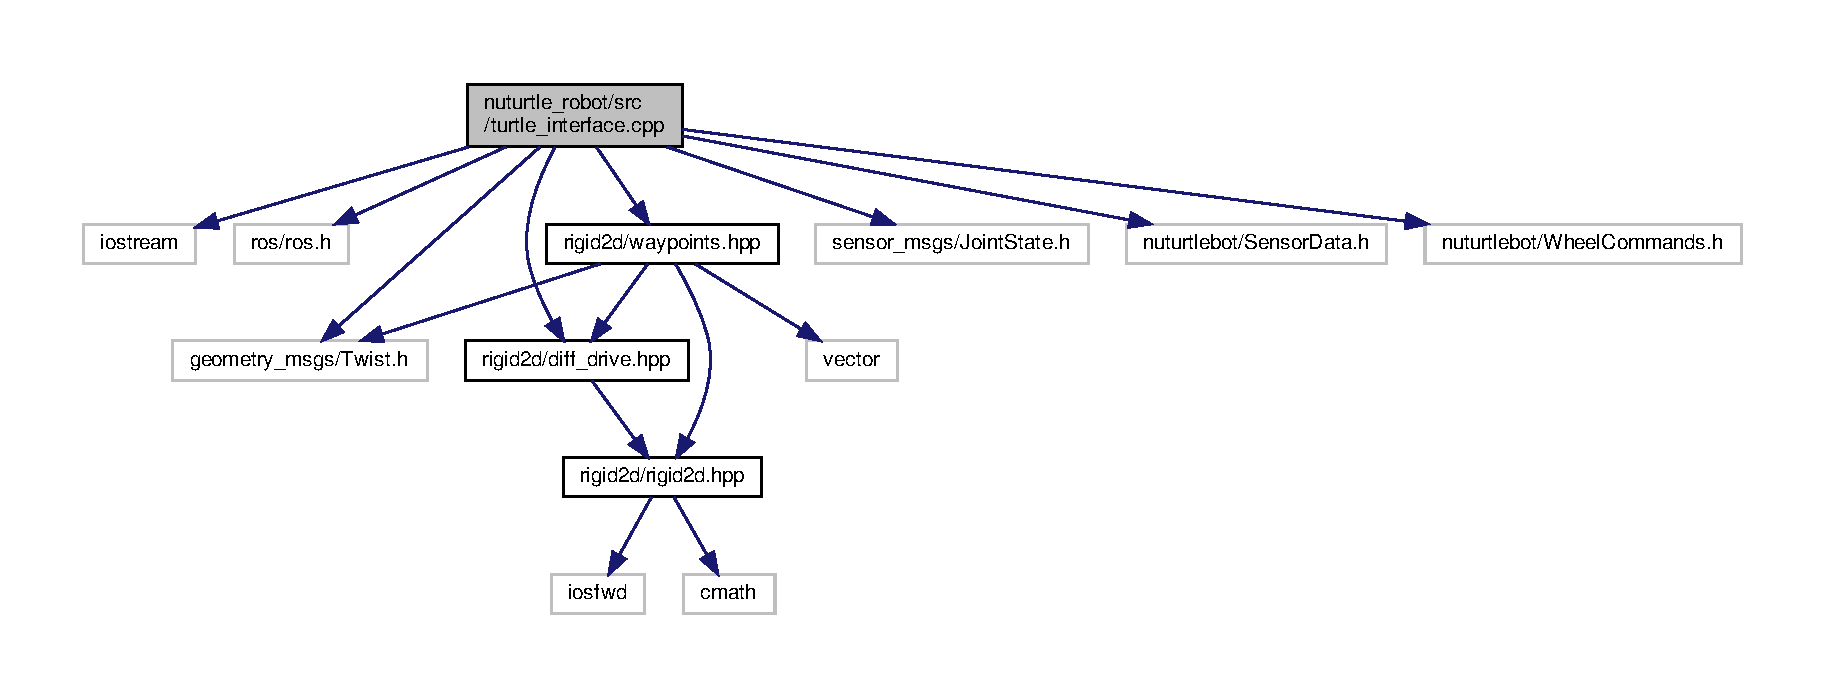
\includegraphics[width=350pt]{d5/d71/turtle__interface_8cpp__incl}
\end{center}
\end{figure}
\subsection*{Functions}
\begin{DoxyCompactItemize}
\item 
\mbox{\Hypertarget{turtle__interface_8cpp_aa32dbd2ab8d28b3c08460b9f2a3d62c7}\label{turtle__interface_8cpp_aa32dbd2ab8d28b3c08460b9f2a3d62c7}} 
void \hyperlink{turtle__interface_8cpp_aa32dbd2ab8d28b3c08460b9f2a3d62c7}{pub\+Wheel\+Commands} ()
\begin{DoxyCompactList}\small\item\em Calculates the proper wheel command given a twist. \end{DoxyCompactList}\item 
\mbox{\Hypertarget{turtle__interface_8cpp_a44c94965143735655ba35b308a070518}\label{turtle__interface_8cpp_a44c94965143735655ba35b308a070518}} 
void \hyperlink{turtle__interface_8cpp_a44c94965143735655ba35b308a070518}{callback\+\_\+twist} (geometry\+\_\+msgs\+::\+Twist\+::\+Const\+Ptr data)
\begin{DoxyCompactList}\small\item\em callback funtion for the cmd\+\_\+vel subscriber \end{DoxyCompactList}\item 
\mbox{\Hypertarget{turtle__interface_8cpp_af39206c46f7e964bd309340466518ee3}\label{turtle__interface_8cpp_af39206c46f7e964bd309340466518ee3}} 
void \hyperlink{turtle__interface_8cpp_af39206c46f7e964bd309340466518ee3}{callback\+\_\+sensors} (nuturtlebot\+::\+Sensor\+Data\+::\+Const\+Ptr data)
\begin{DoxyCompactList}\small\item\em callback funtion for the sensor\+\_\+data subscriber \end{DoxyCompactList}\item 
\mbox{\Hypertarget{turtle__interface_8cpp_a3c04138a5bfe5d72780bb7e82a18e627}\label{turtle__interface_8cpp_a3c04138a5bfe5d72780bb7e82a18e627}} 
int \hyperlink{turtle__interface_8cpp_a3c04138a5bfe5d72780bb7e82a18e627}{main} (int argc, char $\ast$$\ast$argv)
\begin{DoxyCompactList}\small\item\em Main function to create the turtle\+\_\+interface node. \end{DoxyCompactList}\end{DoxyCompactItemize}


\subsection{Detailed Description}
This node interfaces between a main computer and the raspberri pi on the turtlebot. 

P\+A\+R\+A\+M\+E\+T\+E\+RS\+: left\+\_\+wheel\+\_\+joint (std\+::string)\+: the name of the left wheel joint right\+\_\+wheel\+\_\+joint (std\+::string)\+: the name of the right wheel joint wheel\+\_\+base (double)\+: the distance between the two wheels of the diff drive robot wheel\+\_\+radius (double)\+: the radius of the wheels frequency (double)\+: the frequency to publish joint states at tvel\+\_\+lim (double)\+: the maximum translational velocity avel\+\_\+lim (double)\+: the maximum angular velocity motor\+\_\+lim (double)\+: the maximum rotation velocity of the motor encoder\+\_\+ticks\+\_\+per\+\_\+rev (int)\+: the number of encoder pulses per revolution of the wheel motor\+\_\+power (int)\+: the max command value to send the motor P\+U\+B\+L\+I\+S\+H\+ES\+: /wheel\+\_\+cmd (nuturtlebot/\+Wheel\+Commands)\+: a command to control the motors on the turtlebot /joint\+\_\+states (sensor\+\_\+msgs/\+Joint\+State)\+: the wheel position and velocities of the turtlebot S\+U\+B\+S\+C\+R\+I\+B\+ES\+: /cmd\+\_\+vel (geometry\+\_\+msgs/\+Twist)\+: the twist command from the turtlesim package /sensor\+\_\+data (nuturtlebot/\+Sensor\+Data)\+: retrives sensor info from the turtlebot 
\hypertarget{diff__drive_8hpp}{}\section{rigid2d/include/rigid2d/diff\+\_\+drive.hpp File Reference}
\label{diff__drive_8hpp}\index{rigid2d/include/rigid2d/diff\+\_\+drive.\+hpp@{rigid2d/include/rigid2d/diff\+\_\+drive.\+hpp}}


Library for tracking the state of a diff drive robot.  


{\ttfamily \#include \char`\"{}rigid2d/rigid2d.\+hpp\char`\"{}}\newline
Include dependency graph for diff\+\_\+drive.\+hpp\+:
\nopagebreak
\begin{figure}[H]
\begin{center}
\leavevmode
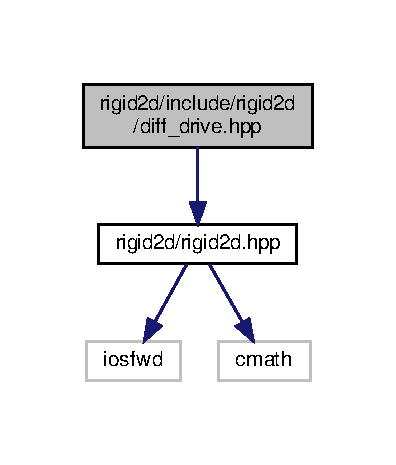
\includegraphics[width=190pt]{dd/d54/diff__drive_8hpp__incl}
\end{center}
\end{figure}
This graph shows which files directly or indirectly include this file\+:
\nopagebreak
\begin{figure}[H]
\begin{center}
\leavevmode
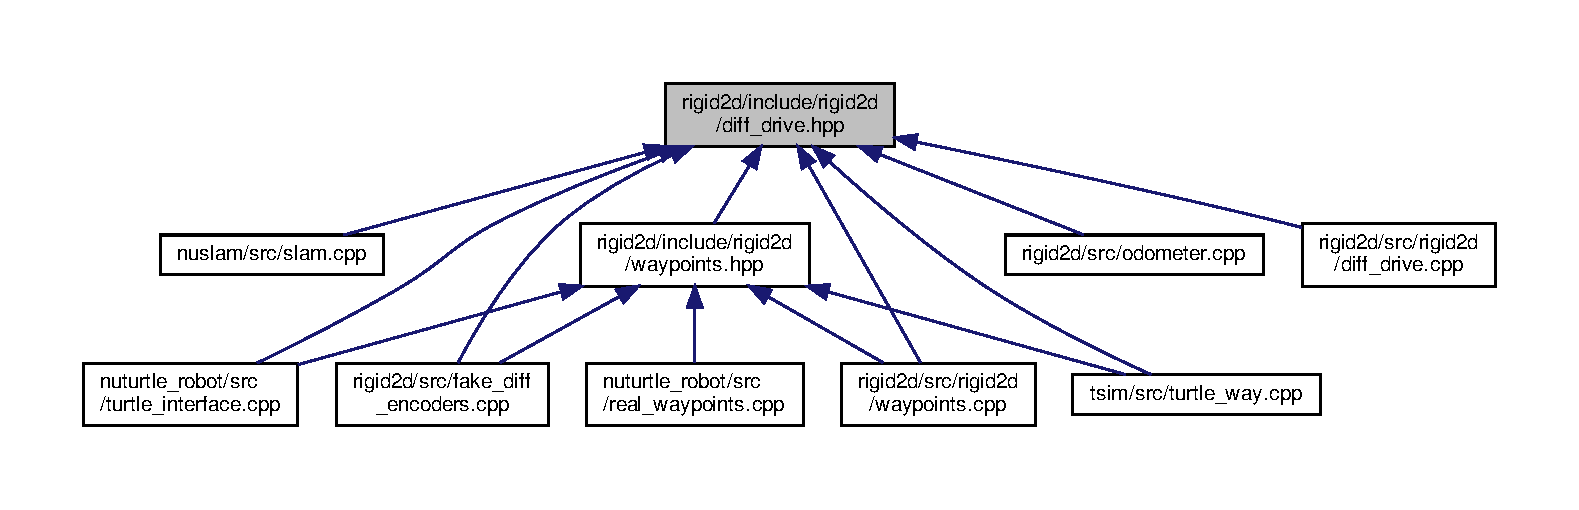
\includegraphics[width=350pt]{dc/d97/diff__drive_8hpp__dep__incl}
\end{center}
\end{figure}
\subsection*{Classes}
\begin{DoxyCompactItemize}
\item 
struct \hyperlink{structrigid2d_1_1WheelVelocities}{rigid2d\+::\+Wheel\+Velocities}
\begin{DoxyCompactList}\small\item\em Wheel velocities for a diff drive robot. \end{DoxyCompactList}\item 
class \hyperlink{classrigid2d_1_1DiffDrive}{rigid2d\+::\+Diff\+Drive}
\end{DoxyCompactItemize}


\subsection{Detailed Description}
Library for tracking the state of a diff drive robot. 


\hypertarget{rigid2d_8hpp}{}\section{rigid2d/include/rigid2d/rigid2d.hpp File Reference}
\label{rigid2d_8hpp}\index{rigid2d/include/rigid2d/rigid2d.\+hpp@{rigid2d/include/rigid2d/rigid2d.\+hpp}}


Library for two-\/dimensional rigid body transformations.  


{\ttfamily \#include $<$iosfwd$>$}\newline
{\ttfamily \#include $<$cmath$>$}\newline
Include dependency graph for rigid2d.\+hpp\+:
\nopagebreak
\begin{figure}[H]
\begin{center}
\leavevmode
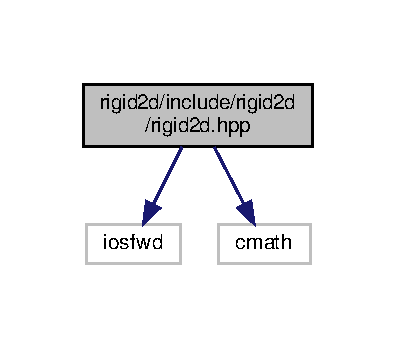
\includegraphics[width=190pt]{d9/d5e/rigid2d_8hpp__incl}
\end{center}
\end{figure}
This graph shows which files directly or indirectly include this file\+:
\nopagebreak
\begin{figure}[H]
\begin{center}
\leavevmode
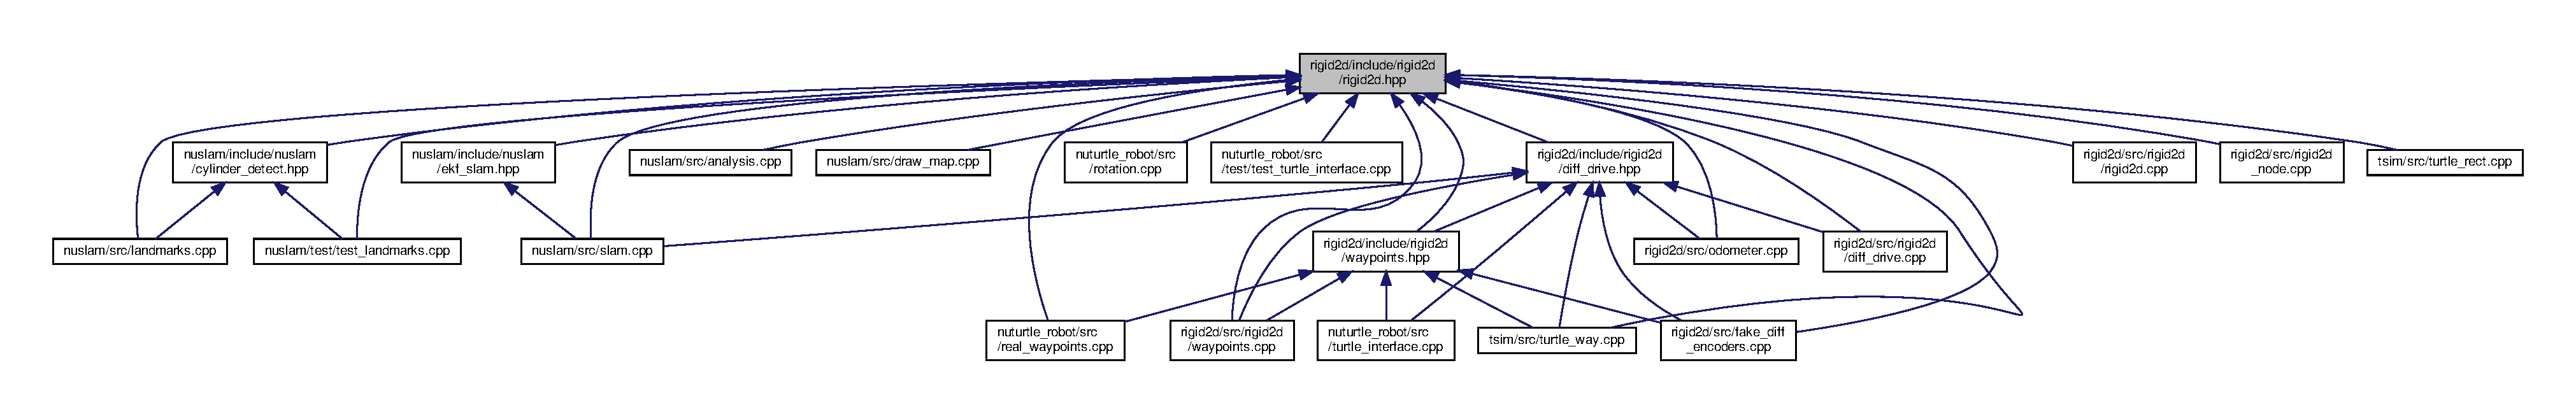
\includegraphics[width=350pt]{dc/ddb/rigid2d_8hpp__dep__incl}
\end{center}
\end{figure}
\subsection*{Classes}
\begin{DoxyCompactItemize}
\item 
struct \hyperlink{structrigid2d_1_1Vector2D}{rigid2d\+::\+Vector2D}
\begin{DoxyCompactList}\small\item\em A 2-\/\+Dimensional Vector. \end{DoxyCompactList}\item 
struct \hyperlink{structrigid2d_1_1Twist2D}{rigid2d\+::\+Twist2D}
\begin{DoxyCompactList}\small\item\em A 2-\/\+Dimensional Twist. \end{DoxyCompactList}\item 
struct \hyperlink{structrigid2d_1_1Pose2D}{rigid2d\+::\+Pose2D}
\begin{DoxyCompactList}\small\item\em A 2-\/\+Dimensional Pose. \end{DoxyCompactList}\item 
class \hyperlink{classrigid2d_1_1Transform2D}{rigid2d\+::\+Transform2D}
\begin{DoxyCompactList}\small\item\em a rigid body transformation in 2 dimensions \end{DoxyCompactList}\end{DoxyCompactItemize}
\subsection*{Functions}
\begin{DoxyCompactItemize}
\item 
constexpr bool \hyperlink{rigid2d_8hpp_aa56fa40a409082af8395dbd4e1a25b1b}{rigid2d\+::almost\+\_\+equal} (double d1, double d2, double epsilon=1.\+0e-\/12)
\begin{DoxyCompactList}\small\item\em approximately compare two floating-\/point numbers using an absolute comparison \end{DoxyCompactList}\item 
constexpr double \hyperlink{rigid2d_8hpp_a58a218146f51c0c2454e5fe1a83cb04c}{rigid2d\+::deg2rad} (double deg)
\begin{DoxyCompactList}\small\item\em convert degrees to radians \end{DoxyCompactList}\item 
constexpr double \hyperlink{rigid2d_8hpp_a6883dbf1c0018c962e890754e9d5f62f}{rigid2d\+::rad2deg} (double rad)
\begin{DoxyCompactList}\small\item\em convert radians to degrees \end{DoxyCompactList}\item 
constexpr double \hyperlink{rigid2d_8hpp_a0366e0678d25f256b74525151b28b1e0}{rigid2d\+::normalize\+\_\+angle} (double rad)
\begin{DoxyCompactList}\small\item\em maps an angle to the range \mbox{[}-\/pi, pi) \end{DoxyCompactList}\item 
constexpr double \hyperlink{rigid2d_8hpp_aff95bc5b895478d464a8424063ed6de4}{rigid2d\+::lin\+Interp} (double x, const double xlims\mbox{[}$\,$\mbox{]}, const double ylims\mbox{[}$\,$\mbox{]})
\begin{DoxyCompactList}\small\item\em Linear Interpolation function. \end{DoxyCompactList}\item 
Vector2D \hyperlink{rigid2d_8hpp_ab95aed81cda08daff1f578f143356af5}{rigid2d\+::operator+} (Vector2D lhs, const Vector2D \&rhs)
\begin{DoxyCompactList}\small\item\em add two vectors together, returning their composition \end{DoxyCompactList}\item 
Vector2D \hyperlink{rigid2d_8hpp_a05afe9efdfd7e1d908b43fb110eacd0a}{rigid2d\+::operator-\/} (Vector2D lhs, const Vector2D \&rhs)
\begin{DoxyCompactList}\small\item\em subtract two vectors together, returning their composition \end{DoxyCompactList}\item 
Vector2D \hyperlink{rigid2d_8hpp_a9181a2dd89fe44f433e4796d135c06d1}{rigid2d\+::operator$\ast$} (Vector2D lhs, const Vector2D \&rhs)
\begin{DoxyCompactList}\small\item\em multiply(scalar) two vectors together, returning their composition \end{DoxyCompactList}\item 
\mbox{\Hypertarget{rigid2d_8hpp_ad6225047f92d9b508ea8169ac629a33d}\label{rigid2d_8hpp_ad6225047f92d9b508ea8169ac629a33d}} 
std\+::ostream \& \hyperlink{rigid2d_8hpp_ad6225047f92d9b508ea8169ac629a33d}{rigid2d\+::operator$<$$<$} (std\+::ostream \&os, const Vector2D \&v)
\begin{DoxyCompactList}\small\item\em output a 2 dimensional vector as \mbox{[}xcomponent ycomponent\mbox{]} os -\/ stream to output to v -\/ the vector to print \end{DoxyCompactList}\item 
\mbox{\Hypertarget{rigid2d_8hpp_a6be2725ac611fb926359452705a2a78b}\label{rigid2d_8hpp_a6be2725ac611fb926359452705a2a78b}} 
std\+::istream \& \hyperlink{rigid2d_8hpp_a6be2725ac611fb926359452705a2a78b}{rigid2d\+::operator$>$$>$} (std\+::istream \&is, Vector2D \&v)
\begin{DoxyCompactList}\small\item\em input a 2 dimensional vector You should be able to read vectors entered as two numbers separated by a newline or a space, or entered as \mbox{[}xcomponent ycomponent\mbox{]} is -\/ stream from which to read v \mbox{[}out\mbox{]} -\/ output vector Hint\+: The following may be useful\+: \href{https://en.cppreference.com/w/cpp/io/basic_istream/peek}{\tt https\+://en.\+cppreference.\+com/w/cpp/io/basic\+\_\+istream/peek} \href{https://en.cppreference.com/w/cpp/io/basic_istream/get}{\tt https\+://en.\+cppreference.\+com/w/cpp/io/basic\+\_\+istream/get} \end{DoxyCompactList}\item 
\mbox{\Hypertarget{rigid2d_8hpp_ac5c87da47bdcc94113443c120872aa2f}\label{rigid2d_8hpp_ac5c87da47bdcc94113443c120872aa2f}} 
std\+::ostream \& \hyperlink{rigid2d_8hpp_ac5c87da47bdcc94113443c120872aa2f}{rigid2d\+::operator$<$$<$} (std\+::ostream \&os, const Twist2D \&tw)
\begin{DoxyCompactList}\small\item\em output a 2 dimensional twist as \mbox{[}wx wy vx vy\mbox{]} os -\/ stream to output to tw -\/ the twist to print \end{DoxyCompactList}\item 
\mbox{\Hypertarget{rigid2d_8hpp_ab3dbb63aa66f6e11552fa74402b74166}\label{rigid2d_8hpp_ab3dbb63aa66f6e11552fa74402b74166}} 
std\+::istream \& \hyperlink{rigid2d_8hpp_ab3dbb63aa66f6e11552fa74402b74166}{rigid2d\+::operator$>$$>$} (std\+::istream \&is, Twist2D \&tw)
\begin{DoxyCompactList}\small\item\em input a 2 dimensional twist tw \mbox{[}out\mbox{]} -\/ output twist \end{DoxyCompactList}\item 
Transform2D \hyperlink{rigid2d_8hpp_a49fcfeea66e35833abb25774a2e58612}{rigid2d\+::transform\+From\+Twist} (Twist2D tw)
\begin{DoxyCompactList}\small\item\em Compute the transform relative to the initial position after following the given twist. \end{DoxyCompactList}\item 
std\+::ostream \& \hyperlink{rigid2d_8hpp_aa6e4ecc06706f3e94aaebb9ba4598d30}{rigid2d\+::operator$<$$<$} (std\+::ostream \&os, const Transform2D \&tf)
\begin{DoxyCompactList}\small\item\em should print a human readable version of the transform\+: An example output\+: dtheta (degrees)\+: 90 dx\+: 3 dy\+: 5 \end{DoxyCompactList}\item 
\mbox{\Hypertarget{rigid2d_8hpp_aa8a4c013498f57be323a74a4a39d7355}\label{rigid2d_8hpp_aa8a4c013498f57be323a74a4a39d7355}} 
std\+::istream \& \hyperlink{rigid2d_8hpp_aa8a4c013498f57be323a74a4a39d7355}{rigid2d\+::operator$>$$>$} (std\+::istream \&is, Transform2D \&tf)
\begin{DoxyCompactList}\small\item\em Read a transformation from stdin Should be able to read input either as output by operator$<$$<$ or as 3 numbers (degrees, dx, dy) separated by spaces or newlines. \end{DoxyCompactList}\item 
Transform2D \hyperlink{rigid2d_8hpp_aed5e0a41db1d3ae524adbb2d7b084a5d}{rigid2d\+::operator$\ast$} (Transform2D lhs, const Transform2D \&rhs)
\begin{DoxyCompactList}\small\item\em multiply two transforms together, returning their composition \end{DoxyCompactList}\end{DoxyCompactItemize}
\subsection*{Variables}
\begin{DoxyCompactItemize}
\item 
\mbox{\Hypertarget{rigid2d_8hpp_af68d2597a40a3021e2c66d1c23019952}\label{rigid2d_8hpp_af68d2597a40a3021e2c66d1c23019952}} 
constexpr double \hyperlink{rigid2d_8hpp_af68d2597a40a3021e2c66d1c23019952}{rigid2d\+::\+PI} =3.\+14159265358979323846
\begin{DoxyCompactList}\small\item\em PI. Not in C++ standard until C++20. \end{DoxyCompactList}\end{DoxyCompactItemize}


\subsection{Detailed Description}
Library for two-\/dimensional rigid body transformations. 



\subsection{Function Documentation}
\mbox{\Hypertarget{rigid2d_8hpp_file_aa56fa40a409082af8395dbd4e1a25b1b}\label{rigid2d_8hpp_file_aa56fa40a409082af8395dbd4e1a25b1b}} 
\index{rigid2d.\+hpp@{rigid2d.\+hpp}!almost\+\_\+equal@{almost\+\_\+equal}}
\index{almost\+\_\+equal@{almost\+\_\+equal}!rigid2d.\+hpp@{rigid2d.\+hpp}}
\subsubsection{\texorpdfstring{almost\+\_\+equal()}{almost\_equal()}}
{\footnotesize\ttfamily constexpr bool rigid2d\+::almost\+\_\+equal (\begin{DoxyParamCaption}\item[{double}]{d1,  }\item[{double}]{d2,  }\item[{double}]{epsilon = {\ttfamily 1.0e-\/12} }\end{DoxyParamCaption})}



approximately compare two floating-\/point numbers using an absolute comparison 


\begin{DoxyParams}{Parameters}
{\em d1} & -\/ a number to compare \\
\hline
{\em d2} & -\/ a second number to compare \\
\hline
{\em epsilon} & -\/ absolute threshold required for equality \\
\hline
\end{DoxyParams}
\begin{DoxyReturn}{Returns}
true if abs(d1 -\/ d2) $<$ epsilon Note\+: the fabs function in $<$cmath$>$ (c++ equivalent of math.\+h) will be useful here 
\end{DoxyReturn}
\mbox{\Hypertarget{rigid2d_8hpp_file_a58a218146f51c0c2454e5fe1a83cb04c}\label{rigid2d_8hpp_file_a58a218146f51c0c2454e5fe1a83cb04c}} 
\index{rigid2d.\+hpp@{rigid2d.\+hpp}!deg2rad@{deg2rad}}
\index{deg2rad@{deg2rad}!rigid2d.\+hpp@{rigid2d.\+hpp}}
\subsubsection{\texorpdfstring{deg2rad()}{deg2rad()}}
{\footnotesize\ttfamily constexpr double rigid2d\+::deg2rad (\begin{DoxyParamCaption}\item[{double}]{deg }\end{DoxyParamCaption})}



convert degrees to radians 


\begin{DoxyParams}{Parameters}
{\em deg} & -\/ angle in degrees \\
\hline
\end{DoxyParams}
\begin{DoxyReturn}{Returns}
radians N\+O\+TE\+: implement this in the header file constexpr means that the function can be computed at compile time if given a compile-\/time constant as input 
\end{DoxyReturn}
\mbox{\Hypertarget{rigid2d_8hpp_file_aff95bc5b895478d464a8424063ed6de4}\label{rigid2d_8hpp_file_aff95bc5b895478d464a8424063ed6de4}} 
\index{rigid2d.\+hpp@{rigid2d.\+hpp}!lin\+Interp@{lin\+Interp}}
\index{lin\+Interp@{lin\+Interp}!rigid2d.\+hpp@{rigid2d.\+hpp}}
\subsubsection{\texorpdfstring{lin\+Interp()}{linInterp()}}
{\footnotesize\ttfamily constexpr double rigid2d\+::lin\+Interp (\begin{DoxyParamCaption}\item[{double}]{x,  }\item[{const double}]{xlims\mbox{[}$\,$\mbox{]},  }\item[{const double}]{ylims\mbox{[}$\,$\mbox{]} }\end{DoxyParamCaption})}



Linear Interpolation function. 


\begin{DoxyParams}{Parameters}
{\em x} & value to interpolate from xlims to ylims \\
\hline
{\em xlims} & limits for the input range \\
\hline
{\em ylims} & limits for the output range \\
\hline
\end{DoxyParams}
\begin{DoxyReturn}{Returns}
angle mapped to the range \mbox{[}-\/pi, pi) 
\end{DoxyReturn}
\mbox{\Hypertarget{rigid2d_8hpp_file_a0366e0678d25f256b74525151b28b1e0}\label{rigid2d_8hpp_file_a0366e0678d25f256b74525151b28b1e0}} 
\index{rigid2d.\+hpp@{rigid2d.\+hpp}!normalize\+\_\+angle@{normalize\+\_\+angle}}
\index{normalize\+\_\+angle@{normalize\+\_\+angle}!rigid2d.\+hpp@{rigid2d.\+hpp}}
\subsubsection{\texorpdfstring{normalize\+\_\+angle()}{normalize\_angle()}}
{\footnotesize\ttfamily constexpr double rigid2d\+::normalize\+\_\+angle (\begin{DoxyParamCaption}\item[{double}]{rad }\end{DoxyParamCaption})}



maps an angle to the range \mbox{[}-\/pi, pi) 


\begin{DoxyParams}{Parameters}
{\em rad} & -\/ any angle \\
\hline
\end{DoxyParams}
\begin{DoxyReturn}{Returns}
angle mapped to the range \mbox{[}-\/pi, pi) 
\end{DoxyReturn}
\mbox{\Hypertarget{rigid2d_8hpp_file_a9181a2dd89fe44f433e4796d135c06d1}\label{rigid2d_8hpp_file_a9181a2dd89fe44f433e4796d135c06d1}} 
\index{rigid2d.\+hpp@{rigid2d.\+hpp}!operator$\ast$@{operator$\ast$}}
\index{operator$\ast$@{operator$\ast$}!rigid2d.\+hpp@{rigid2d.\+hpp}}
\subsubsection{\texorpdfstring{operator$\ast$()}{operator*()}\hspace{0.1cm}{\footnotesize\ttfamily [1/2]}}
{\footnotesize\ttfamily Vector2D rigid2d\+::operator$\ast$ (\begin{DoxyParamCaption}\item[{\hyperlink{structrigid2d_1_1Vector2D}{Vector2D}}]{lhs,  }\item[{const \hyperlink{structrigid2d_1_1Vector2D}{Vector2D} \&}]{rhs }\end{DoxyParamCaption})}



multiply(scalar) two vectors together, returning their composition 


\begin{DoxyParams}{Parameters}
{\em lhs} & -\/ the left hand operand \\
\hline
{\em rhs} & -\/ the right hand operand \\
\hline
\end{DoxyParams}
\begin{DoxyReturn}{Returns}
the composition of the two vectors 
\end{DoxyReturn}
\mbox{\Hypertarget{rigid2d_8hpp_file_aed5e0a41db1d3ae524adbb2d7b084a5d}\label{rigid2d_8hpp_file_aed5e0a41db1d3ae524adbb2d7b084a5d}} 
\index{rigid2d.\+hpp@{rigid2d.\+hpp}!operator$\ast$@{operator$\ast$}}
\index{operator$\ast$@{operator$\ast$}!rigid2d.\+hpp@{rigid2d.\+hpp}}
\subsubsection{\texorpdfstring{operator$\ast$()}{operator*()}\hspace{0.1cm}{\footnotesize\ttfamily [2/2]}}
{\footnotesize\ttfamily Transform2D rigid2d\+::operator$\ast$ (\begin{DoxyParamCaption}\item[{\hyperlink{classrigid2d_1_1Transform2D}{Transform2D}}]{lhs,  }\item[{const \hyperlink{classrigid2d_1_1Transform2D}{Transform2D} \&}]{rhs }\end{DoxyParamCaption})}



multiply two transforms together, returning their composition 


\begin{DoxyParams}{Parameters}
{\em lhs} & -\/ the left hand operand \\
\hline
{\em rhs} & -\/ the right hand operand \\
\hline
\end{DoxyParams}
\begin{DoxyReturn}{Returns}
the composition of the two transforms 
\end{DoxyReturn}
\mbox{\Hypertarget{rigid2d_8hpp_file_ab95aed81cda08daff1f578f143356af5}\label{rigid2d_8hpp_file_ab95aed81cda08daff1f578f143356af5}} 
\index{rigid2d.\+hpp@{rigid2d.\+hpp}!operator+@{operator+}}
\index{operator+@{operator+}!rigid2d.\+hpp@{rigid2d.\+hpp}}
\subsubsection{\texorpdfstring{operator+()}{operator+()}}
{\footnotesize\ttfamily Vector2D rigid2d\+::operator+ (\begin{DoxyParamCaption}\item[{\hyperlink{structrigid2d_1_1Vector2D}{Vector2D}}]{lhs,  }\item[{const \hyperlink{structrigid2d_1_1Vector2D}{Vector2D} \&}]{rhs }\end{DoxyParamCaption})}



add two vectors together, returning their composition 


\begin{DoxyParams}{Parameters}
{\em lhs} & -\/ the left hand operand \\
\hline
{\em rhs} & -\/ the right hand operand \\
\hline
\end{DoxyParams}
\begin{DoxyReturn}{Returns}
the composition of the two vectors 
\end{DoxyReturn}
\mbox{\Hypertarget{rigid2d_8hpp_file_a05afe9efdfd7e1d908b43fb110eacd0a}\label{rigid2d_8hpp_file_a05afe9efdfd7e1d908b43fb110eacd0a}} 
\index{rigid2d.\+hpp@{rigid2d.\+hpp}!operator-\/@{operator-\/}}
\index{operator-\/@{operator-\/}!rigid2d.\+hpp@{rigid2d.\+hpp}}
\subsubsection{\texorpdfstring{operator-\/()}{operator-()}}
{\footnotesize\ttfamily Vector2D rigid2d\+::operator-\/ (\begin{DoxyParamCaption}\item[{\hyperlink{structrigid2d_1_1Vector2D}{Vector2D}}]{lhs,  }\item[{const \hyperlink{structrigid2d_1_1Vector2D}{Vector2D} \&}]{rhs }\end{DoxyParamCaption})}



subtract two vectors together, returning their composition 


\begin{DoxyParams}{Parameters}
{\em lhs} & -\/ the left hand operand \\
\hline
{\em rhs} & -\/ the right hand operand \\
\hline
\end{DoxyParams}
\begin{DoxyReturn}{Returns}
the composition of the two vectors 
\end{DoxyReturn}
\mbox{\Hypertarget{rigid2d_8hpp_file_aa6e4ecc06706f3e94aaebb9ba4598d30}\label{rigid2d_8hpp_file_aa6e4ecc06706f3e94aaebb9ba4598d30}} 
\index{rigid2d.\+hpp@{rigid2d.\+hpp}!operator$<$$<$@{operator$<$$<$}}
\index{operator$<$$<$@{operator$<$$<$}!rigid2d.\+hpp@{rigid2d.\+hpp}}
\subsubsection{\texorpdfstring{operator$<$$<$()}{operator<<()}}
{\footnotesize\ttfamily std\+::ostream \& rigid2d\+::operator$<$$<$ (\begin{DoxyParamCaption}\item[{std\+::ostream \&}]{os,  }\item[{const \hyperlink{classrigid2d_1_1Transform2D}{Transform2D} \&}]{tf }\end{DoxyParamCaption})}



should print a human readable version of the transform\+: An example output\+: dtheta (degrees)\+: 90 dx\+: 3 dy\+: 5 


\begin{DoxyParams}{Parameters}
{\em os} & -\/ an output stream \\
\hline
{\em tf} & -\/ the transform to print \\
\hline
\end{DoxyParams}
\mbox{\Hypertarget{rigid2d_8hpp_file_a6883dbf1c0018c962e890754e9d5f62f}\label{rigid2d_8hpp_file_a6883dbf1c0018c962e890754e9d5f62f}} 
\index{rigid2d.\+hpp@{rigid2d.\+hpp}!rad2deg@{rad2deg}}
\index{rad2deg@{rad2deg}!rigid2d.\+hpp@{rigid2d.\+hpp}}
\subsubsection{\texorpdfstring{rad2deg()}{rad2deg()}}
{\footnotesize\ttfamily constexpr double rigid2d\+::rad2deg (\begin{DoxyParamCaption}\item[{double}]{rad }\end{DoxyParamCaption})}



convert radians to degrees 


\begin{DoxyParams}{Parameters}
{\em rad} & -\/ angle in radians \\
\hline
\end{DoxyParams}
\begin{DoxyReturn}{Returns}
the angle in degrees 
\end{DoxyReturn}
\mbox{\Hypertarget{rigid2d_8hpp_file_a49fcfeea66e35833abb25774a2e58612}\label{rigid2d_8hpp_file_a49fcfeea66e35833abb25774a2e58612}} 
\index{rigid2d.\+hpp@{rigid2d.\+hpp}!transform\+From\+Twist@{transform\+From\+Twist}}
\index{transform\+From\+Twist@{transform\+From\+Twist}!rigid2d.\+hpp@{rigid2d.\+hpp}}
\subsubsection{\texorpdfstring{transform\+From\+Twist()}{transformFromTwist()}}
{\footnotesize\ttfamily Transform2D rigid2d\+::transform\+From\+Twist (\begin{DoxyParamCaption}\item[{\hyperlink{structrigid2d_1_1Twist2D}{Twist2D}}]{tw }\end{DoxyParamCaption})}



Compute the transform relative to the initial position after following the given twist. 


\begin{DoxyParams}{Parameters}
{\em tw} & -\/ the twist to follow \\
\hline
\end{DoxyParams}
\begin{DoxyReturn}{Returns}
the transform relative to the initial position after following the given twist 
\end{DoxyReturn}

\hypertarget{waypoints_8hpp}{}\section{rigid2d/include/rigid2d/waypoints.hpp File Reference}
\label{waypoints_8hpp}\index{rigid2d/include/rigid2d/waypoints.\+hpp@{rigid2d/include/rigid2d/waypoints.\+hpp}}


Library for calculating the velocities to move between waypoints.  


{\ttfamily \#include \char`\"{}rigid2d/rigid2d.\+hpp\char`\"{}}\newline
{\ttfamily \#include \char`\"{}rigid2d/diff\+\_\+drive.\+hpp\char`\"{}}\newline
{\ttfamily \#include $<$vector$>$}\newline
{\ttfamily \#include \char`\"{}geometry\+\_\+msgs/\+Twist.\+h\char`\"{}}\newline
Include dependency graph for waypoints.\+hpp\+:
\nopagebreak
\begin{figure}[H]
\begin{center}
\leavevmode
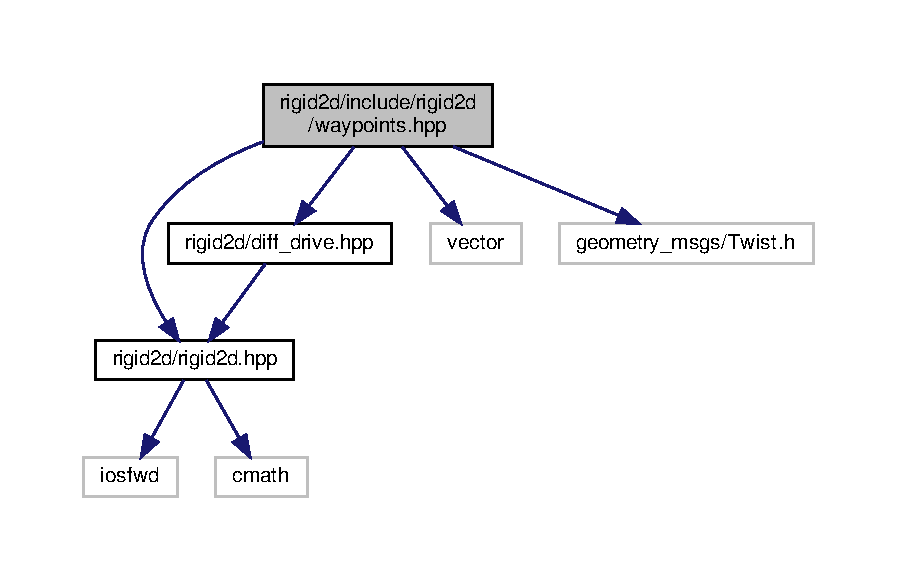
\includegraphics[width=350pt]{d1/d11/waypoints_8hpp__incl}
\end{center}
\end{figure}
This graph shows which files directly or indirectly include this file\+:
\nopagebreak
\begin{figure}[H]
\begin{center}
\leavevmode
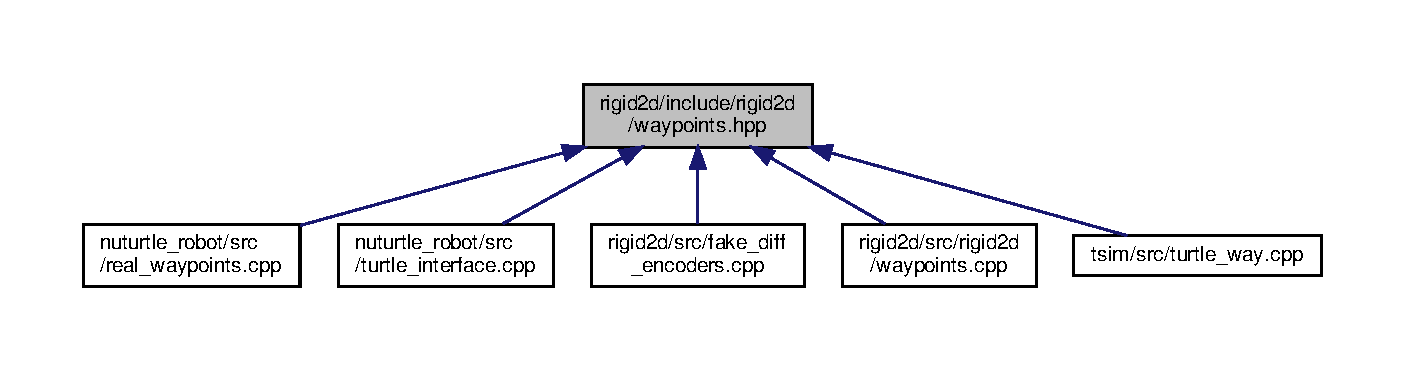
\includegraphics[width=350pt]{d0/d66/waypoints_8hpp__dep__incl}
\end{center}
\end{figure}
\subsection*{Classes}
\begin{DoxyCompactItemize}
\item 
class \hyperlink{classrigid2d_1_1Waypoints}{rigid2d\+::\+Waypoints}
\end{DoxyCompactItemize}
\subsection*{Functions}
\begin{DoxyCompactItemize}
\item 
geometry\+\_\+msgs\+::\+Twist \hyperlink{waypoints_8hpp_a4fb2a740032a89733675537e6816e767}{rigid2d\+::\+Twist2\+Dto\+Geo\+Twist} (Twist2D tw)
\begin{DoxyCompactList}\small\item\em convert a \hyperlink{structrigid2d_1_1Twist2D}{Twist2D} into a geometry\+\_\+msgs\+::\+Twist \end{DoxyCompactList}\item 
Twist2D \hyperlink{waypoints_8hpp_a01bafc1ac1170daac0d7f781eb010d02}{rigid2d\+::\+Geo\+Twistto\+Twist2D} (geometry\+\_\+msgs\+::\+Twist gtw)
\begin{DoxyCompactList}\small\item\em convert a geometry\+\_\+msgs\+::\+Twist into a \hyperlink{structrigid2d_1_1Twist2D}{Twist2D} \end{DoxyCompactList}\end{DoxyCompactItemize}


\subsection{Detailed Description}
Library for calculating the velocities to move between waypoints. 



\subsection{Function Documentation}
\mbox{\Hypertarget{waypoints_8hpp_file_a01bafc1ac1170daac0d7f781eb010d02}\label{waypoints_8hpp_file_a01bafc1ac1170daac0d7f781eb010d02}} 
\index{waypoints.\+hpp@{waypoints.\+hpp}!Geo\+Twistto\+Twist2D@{Geo\+Twistto\+Twist2D}}
\index{Geo\+Twistto\+Twist2D@{Geo\+Twistto\+Twist2D}!waypoints.\+hpp@{waypoints.\+hpp}}
\subsubsection{\texorpdfstring{Geo\+Twistto\+Twist2\+D()}{GeoTwisttoTwist2D()}}
{\footnotesize\ttfamily Twist2D rigid2d\+::\+Geo\+Twistto\+Twist2D (\begin{DoxyParamCaption}\item[{geometry\+\_\+msgs\+::\+Twist}]{gtw }\end{DoxyParamCaption})}



convert a geometry\+\_\+msgs\+::\+Twist into a Twist2D 


\begin{DoxyParams}{Parameters}
{\em twg} & -\/ a geometry\+\_\+msgs\+::\+Twist to convert \\
\hline
\end{DoxyParams}
\begin{DoxyReturn}{Returns}
the equivalent Twist2D 
\end{DoxyReturn}
\mbox{\Hypertarget{waypoints_8hpp_file_a4fb2a740032a89733675537e6816e767}\label{waypoints_8hpp_file_a4fb2a740032a89733675537e6816e767}} 
\index{waypoints.\+hpp@{waypoints.\+hpp}!Twist2\+Dto\+Geo\+Twist@{Twist2\+Dto\+Geo\+Twist}}
\index{Twist2\+Dto\+Geo\+Twist@{Twist2\+Dto\+Geo\+Twist}!waypoints.\+hpp@{waypoints.\+hpp}}
\subsubsection{\texorpdfstring{Twist2\+Dto\+Geo\+Twist()}{Twist2DtoGeoTwist()}}
{\footnotesize\ttfamily geometry\+\_\+msgs\+::\+Twist rigid2d\+::\+Twist2\+Dto\+Geo\+Twist (\begin{DoxyParamCaption}\item[{\hyperlink{structrigid2d_1_1Twist2D}{Twist2D}}]{tw }\end{DoxyParamCaption})}



convert a Twist2D into a geometry\+\_\+msgs\+::\+Twist 


\begin{DoxyParams}{Parameters}
{\em tw} & -\/ a Twist2D to convert \\
\hline
\end{DoxyParams}
\begin{DoxyReturn}{Returns}
the equivalent geometry\+\_\+msgs\+::\+Twist 
\end{DoxyReturn}

\hypertarget{fake__diff__encoders_8cpp}{}\section{rigid2d/src/fake\+\_\+diff\+\_\+encoders.cpp File Reference}
\label{fake__diff__encoders_8cpp}\index{rigid2d/src/fake\+\_\+diff\+\_\+encoders.\+cpp@{rigid2d/src/fake\+\_\+diff\+\_\+encoders.\+cpp}}


This file contains the source code for the turtle\+\_\+rect node. It pulls in parameters set from the yaml file and uses feed forward control to drive the turtle in a rectangle. It also calculates the positional error over time.  


{\ttfamily \#include $<$iostream$>$}\newline
{\ttfamily \#include $<$ros/ros.\+h$>$}\newline
{\ttfamily \#include \char`\"{}geometry\+\_\+msgs/\+Twist.\+h\char`\"{}}\newline
{\ttfamily \#include $<$sensor\+\_\+msgs/\+Joint\+State.\+h$>$}\newline
{\ttfamily \#include \char`\"{}rigid2d/rigid2d.\+hpp\char`\"{}}\newline
{\ttfamily \#include \char`\"{}rigid2d/diff\+\_\+drive.\+hpp\char`\"{}}\newline
{\ttfamily \#include \char`\"{}rigid2d/waypoints.\+hpp\char`\"{}}\newline
Include dependency graph for fake\+\_\+diff\+\_\+encoders.\+cpp\+:
\nopagebreak
\begin{figure}[H]
\begin{center}
\leavevmode
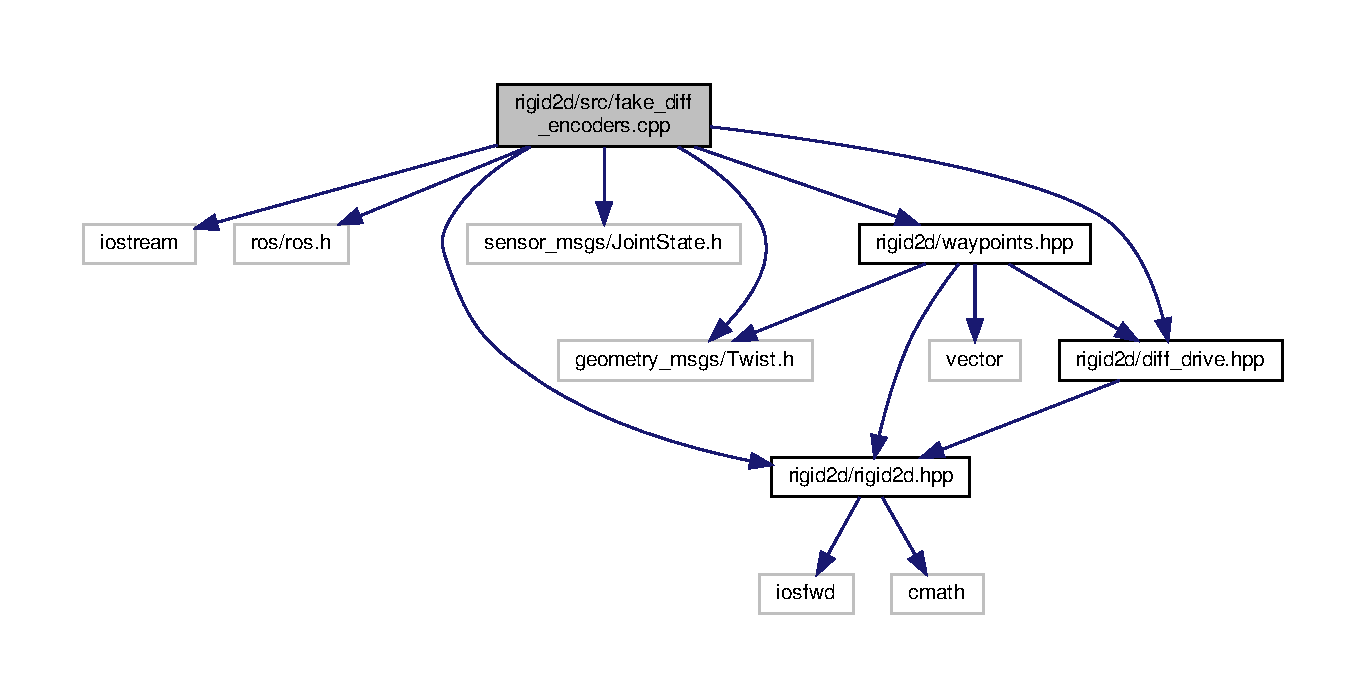
\includegraphics[width=350pt]{dd/d93/fake__diff__encoders_8cpp__incl}
\end{center}
\end{figure}
\subsection*{Functions}
\begin{DoxyCompactItemize}
\item 
\mbox{\Hypertarget{fake__diff__encoders_8cpp_a44c94965143735655ba35b308a070518}\label{fake__diff__encoders_8cpp_a44c94965143735655ba35b308a070518}} 
void \hyperlink{fake__diff__encoders_8cpp_a44c94965143735655ba35b308a070518}{callback\+\_\+twist} (geometry\+\_\+msgs\+::\+Twist\+::\+Const\+Ptr data)
\begin{DoxyCompactList}\small\item\em callback funtion for the /turtle1/cmd\+\_\+vel subscriber \end{DoxyCompactList}\item 
\mbox{\Hypertarget{fake__diff__encoders_8cpp_a3c04138a5bfe5d72780bb7e82a18e627}\label{fake__diff__encoders_8cpp_a3c04138a5bfe5d72780bb7e82a18e627}} 
int \hyperlink{fake__diff__encoders_8cpp_a3c04138a5bfe5d72780bb7e82a18e627}{main} (int argc, char $\ast$$\ast$argv)
\begin{DoxyCompactList}\small\item\em Main function to create the fake\+\_\+diff\+\_\+encoders node. \end{DoxyCompactList}\end{DoxyCompactItemize}


\subsection{Detailed Description}
This file contains the source code for the turtle\+\_\+rect node. It pulls in parameters set from the yaml file and uses feed forward control to drive the turtle in a rectangle. It also calculates the positional error over time. 

P\+A\+R\+A\+M\+E\+T\+E\+RS\+: left\+\_\+wheel\+\_\+joint (std\+::string) the name of the left wheel joint right\+\_\+wheel\+\_\+joint (std\+::string) the name of the right wheel joint wheel\+\_\+base (double) the distance between the two wheels of the diff drive robot wheel\+\_\+radius (double) the radius of the wheels frequency (double) the frequency to publish joint states at P\+U\+B\+L\+I\+S\+H\+ES\+: /joint\+\_\+states (sensor\+\_\+msgs/\+Joint\+State) publishs the scaled wheel velocities and the resulting distance of rotation for wheels moving at that velocity S\+U\+B\+S\+C\+R\+I\+B\+ES\+: /turtle1/cmd\+\_\+vel (geometry\+\_\+msgs/\+Twist)\+: Retrieves the current twist of the turtle 
\hypertarget{odometer_8cpp}{}\section{rigid2d/src/odometer.cpp File Reference}
\label{odometer_8cpp}\index{rigid2d/src/odometer.\+cpp@{rigid2d/src/odometer.\+cpp}}


This node publishes the Odometry messages per R\+OS standard format.  


{\ttfamily \#include $<$iostream$>$}\newline
{\ttfamily \#include $<$ros/ros.\+h$>$}\newline
{\ttfamily \#include $<$tf2\+\_\+ros/transform\+\_\+broadcaster.\+h$>$}\newline
{\ttfamily \#include $<$tf2/\+Linear\+Math/\+Quaternion.\+h$>$}\newline
{\ttfamily \#include $<$tf2\+\_\+geometry\+\_\+msgs/tf2\+\_\+geometry\+\_\+msgs.\+h$>$}\newline
{\ttfamily \#include $<$geometry\+\_\+msgs/\+Transform\+Stamped.\+h$>$}\newline
{\ttfamily \#include $<$geometry\+\_\+msgs/\+Quaternion.\+h$>$}\newline
{\ttfamily \#include $<$nav\+\_\+msgs/\+Odometry.\+h$>$}\newline
{\ttfamily \#include $<$sensor\+\_\+msgs/\+Joint\+State.\+h$>$}\newline
{\ttfamily \#include \char`\"{}rigid2d/\+Set\+Pose.\+h\char`\"{}}\newline
{\ttfamily \#include \char`\"{}rigid2d/rigid2d.\+hpp\char`\"{}}\newline
{\ttfamily \#include \char`\"{}rigid2d/diff\+\_\+drive.\+hpp\char`\"{}}\newline
Include dependency graph for odometer.\+cpp\+:\nopagebreak
\begin{figure}[H]
\begin{center}
\leavevmode
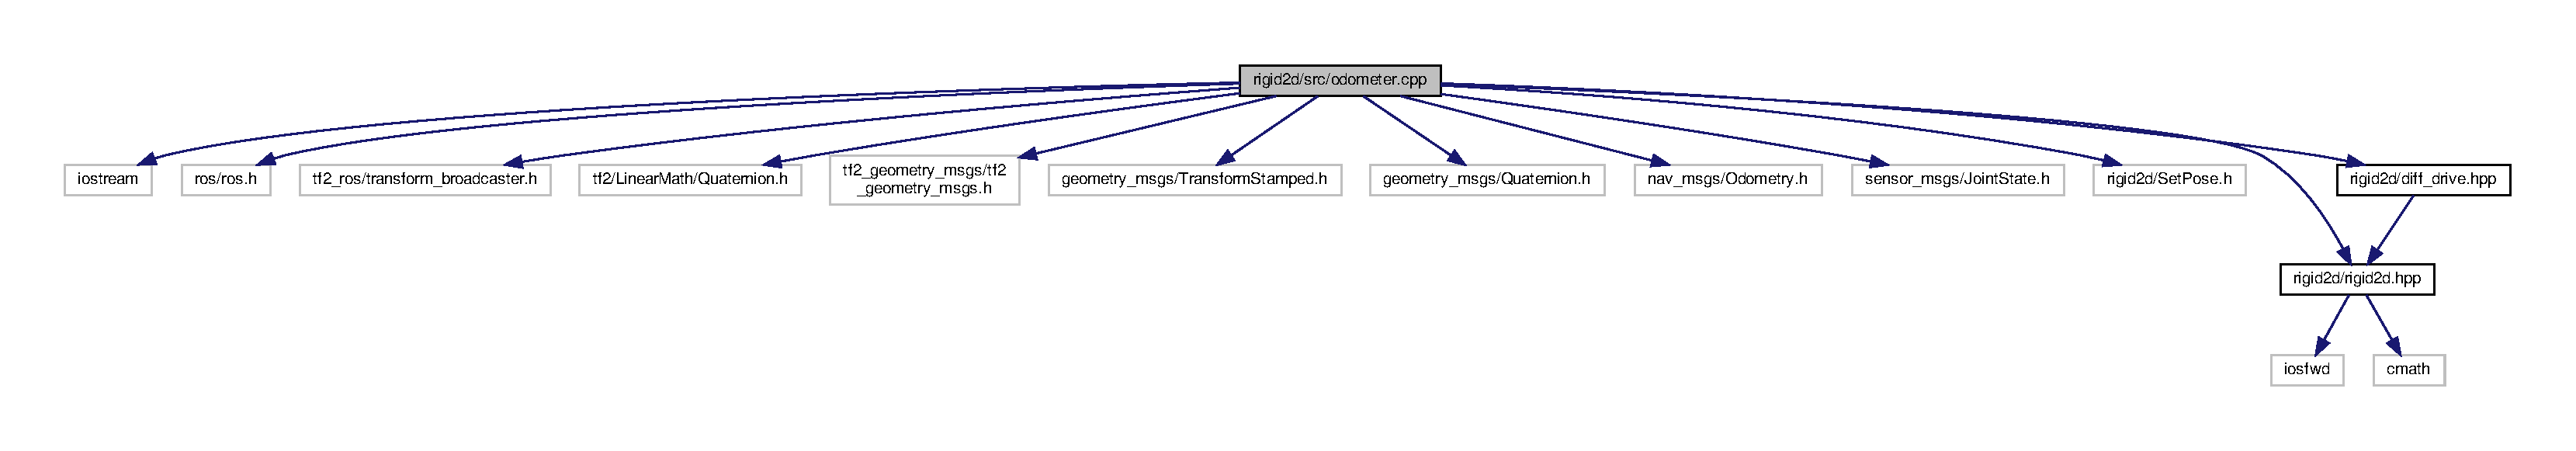
\includegraphics[width=350pt]{d3/d0e/odometer_8cpp__incl}
\end{center}
\end{figure}
\subsection*{Functions}
\begin{DoxyCompactItemize}
\item 
int \hyperlink{odometer_8cpp_ad248270d37c5224dcb705be8b925ff29}{find\+Joint\+Index} (std\+::vector$<$ std\+::string $>$ joints, std\+::string target)
\begin{DoxyCompactList}\small\item\em Use to search through the all joint names and return the index of the desired joint. \end{DoxyCompactList}\item 
\mbox{\Hypertarget{odometer_8cpp_a32393f00b4e0f87fc20fd049f9f29e13}\label{odometer_8cpp_a32393f00b4e0f87fc20fd049f9f29e13}} 
void \hyperlink{odometer_8cpp_a32393f00b4e0f87fc20fd049f9f29e13}{callback\+\_\+joints} (const sensor\+\_\+msgs\+::\+Joint\+State\+::\+Const\+Ptr data)
\begin{DoxyCompactList}\small\item\em Callback for the joint state subscriber. \end{DoxyCompactList}\item 
\mbox{\Hypertarget{odometer_8cpp_aae64b337e2786fc1bc955743eb5921bd}\label{odometer_8cpp_aae64b337e2786fc1bc955743eb5921bd}} 
bool \hyperlink{odometer_8cpp_aae64b337e2786fc1bc955743eb5921bd}{callback\+\_\+set\+\_\+pose} (rigid2d\+::\+Set\+Pose\+::\+Request \&req, rigid2d\+::\+Set\+Pose\+::\+Response \&)
\begin{DoxyCompactList}\small\item\em Callback for the set\+\_\+pose service. \end{DoxyCompactList}\item 
\mbox{\Hypertarget{odometer_8cpp_a3c04138a5bfe5d72780bb7e82a18e627}\label{odometer_8cpp_a3c04138a5bfe5d72780bb7e82a18e627}} 
int \hyperlink{odometer_8cpp_a3c04138a5bfe5d72780bb7e82a18e627}{main} (int argc, char $\ast$$\ast$argv)
\begin{DoxyCompactList}\small\item\em Main function for the odometer node. \end{DoxyCompactList}\end{DoxyCompactItemize}


\subsection{Detailed Description}
This node publishes the Odometry messages per R\+OS standard format. 

P\+A\+R\+A\+M\+E\+T\+E\+RS\+: odom\+\_\+frame\+\_\+id (std\+::string) the name of the odometer frame base\+\_\+frame\+\_\+id (std\+::string) the name of the base frame left\+\_\+wheel\+\_\+joint (std\+::string) the name of the left wheel joint right\+\_\+wheel\+\_\+joint (std\+::string) the name of the right wheel joint wheel\+\_\+base (double) the distance between the two wheels of the diff drive robot wheel\+\_\+radius (double) the radius of the wheels frequency (double) the frequency to publish joint states at P\+U\+B\+L\+I\+S\+H\+ES\+: /odom (nav\+\_\+msgs/\+Odometry)\+: The calculated odometry of the diff drive robot S\+U\+B\+S\+C\+R\+I\+B\+ES\+: /joint\+\_\+states (sensor\+\_\+msgs/\+Joint\+State)\+: Retrieves the calculated wheel velocities and change in wheel position S\+E\+R\+V\+I\+C\+ES\+: /set\+\_\+pose (rigid2d/\+Set\+Pose)\+: Sets the pose of the robot to the provided values 

\subsection{Function Documentation}
\mbox{\Hypertarget{odometer_8cpp_ad248270d37c5224dcb705be8b925ff29}\label{odometer_8cpp_ad248270d37c5224dcb705be8b925ff29}} 
\index{odometer.\+cpp@{odometer.\+cpp}!find\+Joint\+Index@{find\+Joint\+Index}}
\index{find\+Joint\+Index@{find\+Joint\+Index}!odometer.\+cpp@{odometer.\+cpp}}
\subsubsection{\texorpdfstring{find\+Joint\+Index()}{findJointIndex()}}
{\footnotesize\ttfamily int find\+Joint\+Index (\begin{DoxyParamCaption}\item[{std\+::vector$<$ std\+::string $>$}]{joints,  }\item[{std\+::string}]{target }\end{DoxyParamCaption})}



Use to search through the all joint names and return the index of the desired joint. 


\begin{DoxyParams}{Parameters}
{\em joints} & -\/ a vector of all the joint names \\
\hline
{\em target} & -\/ the desire joint name to find \\
\hline
\end{DoxyParams}
\begin{DoxyReturn}{Returns}
the index of the desired joint name 
\end{DoxyReturn}

\hypertarget{diff__drive_8cpp}{}\section{rigid2d/src/rigid2d/diff\+\_\+drive.cpp File Reference}
\label{diff__drive_8cpp}\index{rigid2d/src/rigid2d/diff\+\_\+drive.\+cpp@{rigid2d/src/rigid2d/diff\+\_\+drive.\+cpp}}


Source file for Diff Dirve Robot library.  


{\ttfamily \#include \char`\"{}rigid2d/rigid2d.\+hpp\char`\"{}}\newline
{\ttfamily \#include \char`\"{}rigid2d/diff\+\_\+drive.\+hpp\char`\"{}}\newline
{\ttfamily \#include $<$iostream$>$}\newline
Include dependency graph for diff\+\_\+drive.\+cpp\+:\nopagebreak
\begin{figure}[H]
\begin{center}
\leavevmode
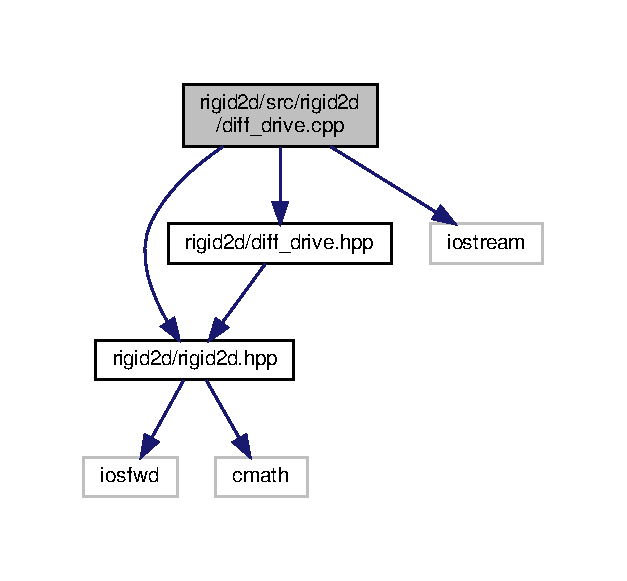
\includegraphics[width=301pt]{dc/d81/diff__drive_8cpp__incl}
\end{center}
\end{figure}


\subsection{Detailed Description}
Source file for Diff Dirve Robot library. 


\hypertarget{rigid2d_8cpp}{}\section{rigid2d/src/rigid2d/rigid2d.cpp File Reference}
\label{rigid2d_8cpp}\index{rigid2d/src/rigid2d/rigid2d.\+cpp@{rigid2d/src/rigid2d/rigid2d.\+cpp}}


Source file for rigid2D 2D Transformation library.  


{\ttfamily \#include $<$iostream$>$}\newline
{\ttfamily \#include \char`\"{}rigid2d/rigid2d.\+hpp\char`\"{}}\newline
Include dependency graph for rigid2d.\+cpp\+:
\nopagebreak
\begin{figure}[H]
\begin{center}
\leavevmode
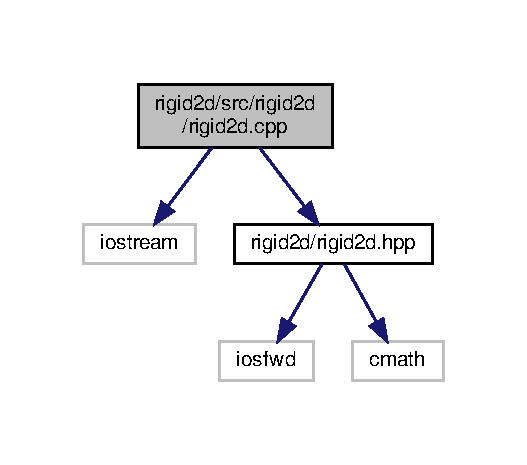
\includegraphics[width=253pt]{dc/dca/rigid2d_8cpp__incl}
\end{center}
\end{figure}
\subsection*{Functions}
\begin{DoxyCompactItemize}
\item 
\mbox{\Hypertarget{rigid2d_8hpp_ad6225047f92d9b508ea8169ac629a33d}\label{rigid2d_8hpp_ad6225047f92d9b508ea8169ac629a33d}} 
std\+::ostream \& \hyperlink{rigid2d_8hpp_ad6225047f92d9b508ea8169ac629a33d}{rigid2d\+::operator$<$$<$} (std\+::ostream \&os, const Vector2D \&v)
\begin{DoxyCompactList}\small\item\em output a 2 dimensional vector as \mbox{[}xcomponent ycomponent\mbox{]} os -\/ stream to output to v -\/ the vector to print \end{DoxyCompactList}\item 
\mbox{\Hypertarget{rigid2d_8hpp_ac5c87da47bdcc94113443c120872aa2f}\label{rigid2d_8hpp_ac5c87da47bdcc94113443c120872aa2f}} 
std\+::ostream \& \hyperlink{rigid2d_8hpp_ac5c87da47bdcc94113443c120872aa2f}{rigid2d\+::operator$<$$<$} (std\+::ostream \&os, const Twist2D \&tw)
\begin{DoxyCompactList}\small\item\em output a 2 dimensional twist as \mbox{[}wx wy vx vy\mbox{]} os -\/ stream to output to tw -\/ the twist to print \end{DoxyCompactList}\item 
std\+::ostream \& \hyperlink{rigid2d_8hpp_aa6e4ecc06706f3e94aaebb9ba4598d30}{rigid2d\+::operator$<$$<$} (std\+::ostream \&os, const Transform2D \&tf)
\begin{DoxyCompactList}\small\item\em should print a human readable version of the transform\+: An example output\+: dtheta (degrees)\+: 90 dx\+: 3 dy\+: 5 \end{DoxyCompactList}\item 
\mbox{\Hypertarget{rigid2d_8hpp_a6be2725ac611fb926359452705a2a78b}\label{rigid2d_8hpp_a6be2725ac611fb926359452705a2a78b}} 
std\+::istream \& \hyperlink{rigid2d_8hpp_a6be2725ac611fb926359452705a2a78b}{rigid2d\+::operator$>$$>$} (std\+::istream \&is, Vector2D \&v)
\begin{DoxyCompactList}\small\item\em input a 2 dimensional vector You should be able to read vectors entered as two numbers separated by a newline or a space, or entered as \mbox{[}xcomponent ycomponent\mbox{]} is -\/ stream from which to read v \mbox{[}out\mbox{]} -\/ output vector Hint\+: The following may be useful\+: \href{https://en.cppreference.com/w/cpp/io/basic_istream/peek}{\tt https\+://en.\+cppreference.\+com/w/cpp/io/basic\+\_\+istream/peek} \href{https://en.cppreference.com/w/cpp/io/basic_istream/get}{\tt https\+://en.\+cppreference.\+com/w/cpp/io/basic\+\_\+istream/get} \end{DoxyCompactList}\item 
\mbox{\Hypertarget{rigid2d_8hpp_ab3dbb63aa66f6e11552fa74402b74166}\label{rigid2d_8hpp_ab3dbb63aa66f6e11552fa74402b74166}} 
std\+::istream \& \hyperlink{rigid2d_8hpp_ab3dbb63aa66f6e11552fa74402b74166}{rigid2d\+::operator$>$$>$} (std\+::istream \&is, Twist2D \&tw)
\begin{DoxyCompactList}\small\item\em input a 2 dimensional twist tw \mbox{[}out\mbox{]} -\/ output twist \end{DoxyCompactList}\item 
\mbox{\Hypertarget{rigid2d_8hpp_aa8a4c013498f57be323a74a4a39d7355}\label{rigid2d_8hpp_aa8a4c013498f57be323a74a4a39d7355}} 
std\+::istream \& \hyperlink{rigid2d_8hpp_aa8a4c013498f57be323a74a4a39d7355}{rigid2d\+::operator$>$$>$} (std\+::istream \&is, Transform2D \&tf)
\begin{DoxyCompactList}\small\item\em Read a transformation from stdin Should be able to read input either as output by operator$<$$<$ or as 3 numbers (degrees, dx, dy) separated by spaces or newlines. \end{DoxyCompactList}\item 
Transform2D \hyperlink{rigid2d_8hpp_a49fcfeea66e35833abb25774a2e58612}{rigid2d\+::transform\+From\+Twist} (Twist2D tw)
\begin{DoxyCompactList}\small\item\em Compute the transform relative to the initial position after following the given twist. \end{DoxyCompactList}\item 
Vector2D \hyperlink{rigid2d_8hpp_ab95aed81cda08daff1f578f143356af5}{rigid2d\+::operator+} (Vector2D lhs, const Vector2D \&rhs)
\begin{DoxyCompactList}\small\item\em add two vectors together, returning their composition \end{DoxyCompactList}\item 
Vector2D \hyperlink{rigid2d_8hpp_a05afe9efdfd7e1d908b43fb110eacd0a}{rigid2d\+::operator-\/} (Vector2D lhs, const Vector2D \&rhs)
\begin{DoxyCompactList}\small\item\em subtract two vectors together, returning their composition \end{DoxyCompactList}\item 
Vector2D \hyperlink{rigid2d_8hpp_a9181a2dd89fe44f433e4796d135c06d1}{rigid2d\+::operator$\ast$} (Vector2D lhs, const Vector2D \&rhs)
\begin{DoxyCompactList}\small\item\em multiply(scalar) two vectors together, returning their composition \end{DoxyCompactList}\item 
Transform2D \hyperlink{rigid2d_8hpp_aed5e0a41db1d3ae524adbb2d7b084a5d}{rigid2d\+::operator$\ast$} (Transform2D lhs, const Transform2D \&rhs)
\begin{DoxyCompactList}\small\item\em multiply two transforms together, returning their composition \end{DoxyCompactList}\end{DoxyCompactItemize}


\subsection{Detailed Description}
Source file for rigid2D 2D Transformation library. 



\subsection{Function Documentation}
\mbox{\Hypertarget{rigid2d_8hpp_file_a9181a2dd89fe44f433e4796d135c06d1}\label{rigid2d_8hpp_file_a9181a2dd89fe44f433e4796d135c06d1}} 
\index{rigid2d.\+cpp@{rigid2d.\+cpp}!operator$\ast$@{operator$\ast$}}
\index{operator$\ast$@{operator$\ast$}!rigid2d.\+cpp@{rigid2d.\+cpp}}
\subsubsection{\texorpdfstring{operator$\ast$()}{operator*()}\hspace{0.1cm}{\footnotesize\ttfamily [1/2]}}
{\footnotesize\ttfamily Vector2D rigid2d\+::operator$\ast$ (\begin{DoxyParamCaption}\item[{\hyperlink{structrigid2d_1_1Vector2D}{Vector2D}}]{lhs,  }\item[{const \hyperlink{structrigid2d_1_1Vector2D}{Vector2D} \&}]{rhs }\end{DoxyParamCaption})}



multiply(scalar) two vectors together, returning their composition 


\begin{DoxyParams}{Parameters}
{\em lhs} & -\/ the left hand operand \\
\hline
{\em rhs} & -\/ the right hand operand \\
\hline
\end{DoxyParams}
\begin{DoxyReturn}{Returns}
the composition of the two vectors 
\end{DoxyReturn}
\mbox{\Hypertarget{rigid2d_8hpp_file_aed5e0a41db1d3ae524adbb2d7b084a5d}\label{rigid2d_8hpp_file_aed5e0a41db1d3ae524adbb2d7b084a5d}} 
\index{rigid2d.\+cpp@{rigid2d.\+cpp}!operator$\ast$@{operator$\ast$}}
\index{operator$\ast$@{operator$\ast$}!rigid2d.\+cpp@{rigid2d.\+cpp}}
\subsubsection{\texorpdfstring{operator$\ast$()}{operator*()}\hspace{0.1cm}{\footnotesize\ttfamily [2/2]}}
{\footnotesize\ttfamily Transform2D rigid2d\+::operator$\ast$ (\begin{DoxyParamCaption}\item[{\hyperlink{classrigid2d_1_1Transform2D}{Transform2D}}]{lhs,  }\item[{const \hyperlink{classrigid2d_1_1Transform2D}{Transform2D} \&}]{rhs }\end{DoxyParamCaption})}



multiply two transforms together, returning their composition 


\begin{DoxyParams}{Parameters}
{\em lhs} & -\/ the left hand operand \\
\hline
{\em rhs} & -\/ the right hand operand \\
\hline
\end{DoxyParams}
\begin{DoxyReturn}{Returns}
the composition of the two transforms 
\end{DoxyReturn}
\mbox{\Hypertarget{rigid2d_8hpp_file_ab95aed81cda08daff1f578f143356af5}\label{rigid2d_8hpp_file_ab95aed81cda08daff1f578f143356af5}} 
\index{rigid2d.\+cpp@{rigid2d.\+cpp}!operator+@{operator+}}
\index{operator+@{operator+}!rigid2d.\+cpp@{rigid2d.\+cpp}}
\subsubsection{\texorpdfstring{operator+()}{operator+()}}
{\footnotesize\ttfamily Vector2D rigid2d\+::operator+ (\begin{DoxyParamCaption}\item[{\hyperlink{structrigid2d_1_1Vector2D}{Vector2D}}]{lhs,  }\item[{const \hyperlink{structrigid2d_1_1Vector2D}{Vector2D} \&}]{rhs }\end{DoxyParamCaption})}



add two vectors together, returning their composition 


\begin{DoxyParams}{Parameters}
{\em lhs} & -\/ the left hand operand \\
\hline
{\em rhs} & -\/ the right hand operand \\
\hline
\end{DoxyParams}
\begin{DoxyReturn}{Returns}
the composition of the two vectors 
\end{DoxyReturn}
\mbox{\Hypertarget{rigid2d_8hpp_file_a05afe9efdfd7e1d908b43fb110eacd0a}\label{rigid2d_8hpp_file_a05afe9efdfd7e1d908b43fb110eacd0a}} 
\index{rigid2d.\+cpp@{rigid2d.\+cpp}!operator-\/@{operator-\/}}
\index{operator-\/@{operator-\/}!rigid2d.\+cpp@{rigid2d.\+cpp}}
\subsubsection{\texorpdfstring{operator-\/()}{operator-()}}
{\footnotesize\ttfamily Vector2D rigid2d\+::operator-\/ (\begin{DoxyParamCaption}\item[{\hyperlink{structrigid2d_1_1Vector2D}{Vector2D}}]{lhs,  }\item[{const \hyperlink{structrigid2d_1_1Vector2D}{Vector2D} \&}]{rhs }\end{DoxyParamCaption})}



subtract two vectors together, returning their composition 


\begin{DoxyParams}{Parameters}
{\em lhs} & -\/ the left hand operand \\
\hline
{\em rhs} & -\/ the right hand operand \\
\hline
\end{DoxyParams}
\begin{DoxyReturn}{Returns}
the composition of the two vectors 
\end{DoxyReturn}
\mbox{\Hypertarget{rigid2d_8hpp_file_aa6e4ecc06706f3e94aaebb9ba4598d30}\label{rigid2d_8hpp_file_aa6e4ecc06706f3e94aaebb9ba4598d30}} 
\index{rigid2d.\+cpp@{rigid2d.\+cpp}!operator$<$$<$@{operator$<$$<$}}
\index{operator$<$$<$@{operator$<$$<$}!rigid2d.\+cpp@{rigid2d.\+cpp}}
\subsubsection{\texorpdfstring{operator$<$$<$()}{operator<<()}}
{\footnotesize\ttfamily std\+::ostream \& rigid2d\+::operator$<$$<$ (\begin{DoxyParamCaption}\item[{std\+::ostream \&}]{os,  }\item[{const \hyperlink{classrigid2d_1_1Transform2D}{Transform2D} \&}]{tf }\end{DoxyParamCaption})}



should print a human readable version of the transform\+: An example output\+: dtheta (degrees)\+: 90 dx\+: 3 dy\+: 5 


\begin{DoxyParams}{Parameters}
{\em os} & -\/ an output stream \\
\hline
{\em tf} & -\/ the transform to print \\
\hline
\end{DoxyParams}
\mbox{\Hypertarget{rigid2d_8hpp_file_a49fcfeea66e35833abb25774a2e58612}\label{rigid2d_8hpp_file_a49fcfeea66e35833abb25774a2e58612}} 
\index{rigid2d.\+cpp@{rigid2d.\+cpp}!transform\+From\+Twist@{transform\+From\+Twist}}
\index{transform\+From\+Twist@{transform\+From\+Twist}!rigid2d.\+cpp@{rigid2d.\+cpp}}
\subsubsection{\texorpdfstring{transform\+From\+Twist()}{transformFromTwist()}}
{\footnotesize\ttfamily Transform2D rigid2d\+::transform\+From\+Twist (\begin{DoxyParamCaption}\item[{\hyperlink{structrigid2d_1_1Twist2D}{Twist2D}}]{tw }\end{DoxyParamCaption})}



Compute the transform relative to the initial position after following the given twist. 


\begin{DoxyParams}{Parameters}
{\em tw} & -\/ the twist to follow \\
\hline
\end{DoxyParams}
\begin{DoxyReturn}{Returns}
the transform relative to the initial position after following the given twist 
\end{DoxyReturn}

\hypertarget{waypoints_8cpp}{}\section{rigid2d/src/rigid2d/waypoints.cpp File Reference}
\label{waypoints_8cpp}\index{rigid2d/src/rigid2d/waypoints.\+cpp@{rigid2d/src/rigid2d/waypoints.\+cpp}}


Library for calculating the velocities to move between waypoints.  


{\ttfamily \#include $<$iostream$>$}\newline
{\ttfamily \#include $<$cmath$>$}\newline
{\ttfamily \#include \char`\"{}geometry\+\_\+msgs/\+Twist.\+h\char`\"{}}\newline
{\ttfamily \#include \char`\"{}rigid2d/rigid2d.\+hpp\char`\"{}}\newline
{\ttfamily \#include \char`\"{}rigid2d/diff\+\_\+drive.\+hpp\char`\"{}}\newline
{\ttfamily \#include \char`\"{}rigid2d/waypoints.\+hpp\char`\"{}}\newline
Include dependency graph for waypoints.\+cpp\+:
\nopagebreak
\begin{figure}[H]
\begin{center}
\leavevmode
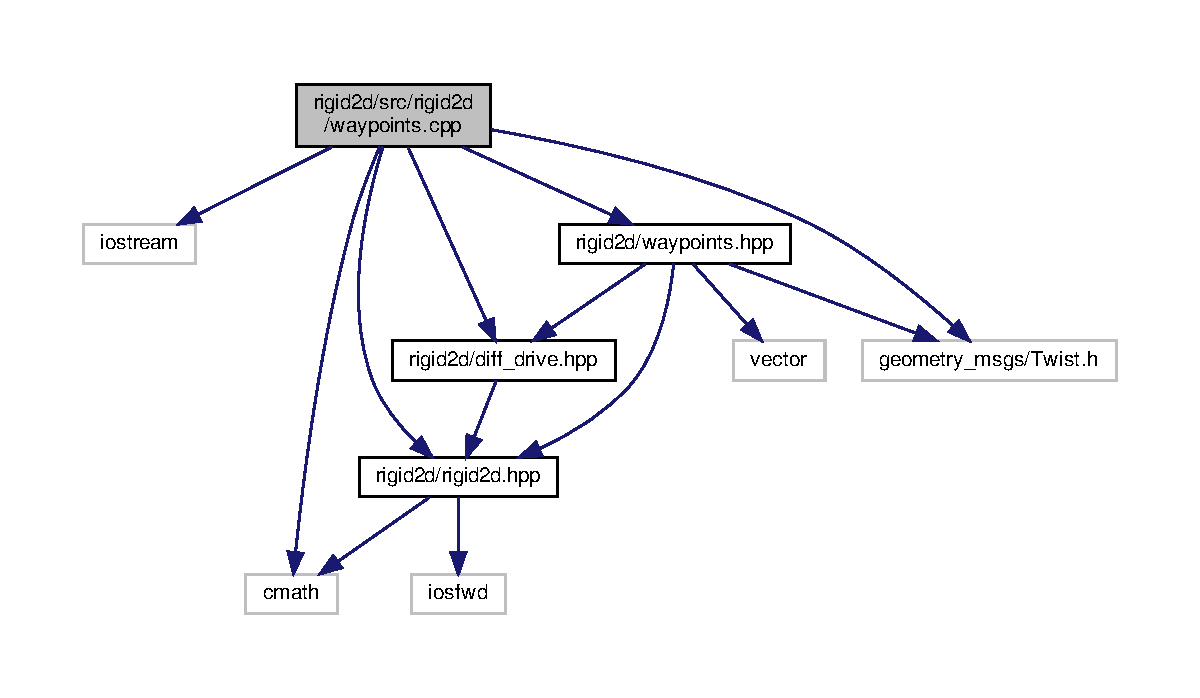
\includegraphics[width=350pt]{d0/db7/waypoints_8cpp__incl}
\end{center}
\end{figure}
\subsection*{Functions}
\begin{DoxyCompactItemize}
\item 
geometry\+\_\+msgs\+::\+Twist \hyperlink{waypoints_8hpp_a4fb2a740032a89733675537e6816e767}{rigid2d\+::\+Twist2\+Dto\+Geo\+Twist} (Twist2D tw)
\begin{DoxyCompactList}\small\item\em convert a \hyperlink{structrigid2d_1_1Twist2D}{Twist2D} into a geometry\+\_\+msgs\+::\+Twist \end{DoxyCompactList}\item 
Twist2D \hyperlink{waypoints_8hpp_a01bafc1ac1170daac0d7f781eb010d02}{rigid2d\+::\+Geo\+Twistto\+Twist2D} (geometry\+\_\+msgs\+::\+Twist gtw)
\begin{DoxyCompactList}\small\item\em convert a geometry\+\_\+msgs\+::\+Twist into a \hyperlink{structrigid2d_1_1Twist2D}{Twist2D} \end{DoxyCompactList}\end{DoxyCompactItemize}


\subsection{Detailed Description}
Library for calculating the velocities to move between waypoints. 



\subsection{Function Documentation}
\mbox{\Hypertarget{waypoints_8hpp_file_a01bafc1ac1170daac0d7f781eb010d02}\label{waypoints_8hpp_file_a01bafc1ac1170daac0d7f781eb010d02}} 
\index{waypoints.\+cpp@{waypoints.\+cpp}!Geo\+Twistto\+Twist2D@{Geo\+Twistto\+Twist2D}}
\index{Geo\+Twistto\+Twist2D@{Geo\+Twistto\+Twist2D}!waypoints.\+cpp@{waypoints.\+cpp}}
\subsubsection{\texorpdfstring{Geo\+Twistto\+Twist2\+D()}{GeoTwisttoTwist2D()}}
{\footnotesize\ttfamily Twist2D rigid2d\+::\+Geo\+Twistto\+Twist2D (\begin{DoxyParamCaption}\item[{geometry\+\_\+msgs\+::\+Twist}]{gtw }\end{DoxyParamCaption})}



convert a geometry\+\_\+msgs\+::\+Twist into a Twist2D 


\begin{DoxyParams}{Parameters}
{\em gtw} & -\/ a geometry\+\_\+msgs\+::\+Twist to convert \\
\hline
\end{DoxyParams}
\begin{DoxyReturn}{Returns}
the equivalent Twist2D 
\end{DoxyReturn}
\mbox{\Hypertarget{waypoints_8hpp_file_a4fb2a740032a89733675537e6816e767}\label{waypoints_8hpp_file_a4fb2a740032a89733675537e6816e767}} 
\index{waypoints.\+cpp@{waypoints.\+cpp}!Twist2\+Dto\+Geo\+Twist@{Twist2\+Dto\+Geo\+Twist}}
\index{Twist2\+Dto\+Geo\+Twist@{Twist2\+Dto\+Geo\+Twist}!waypoints.\+cpp@{waypoints.\+cpp}}
\subsubsection{\texorpdfstring{Twist2\+Dto\+Geo\+Twist()}{Twist2DtoGeoTwist()}}
{\footnotesize\ttfamily geometry\+\_\+msgs\+::\+Twist rigid2d\+::\+Twist2\+Dto\+Geo\+Twist (\begin{DoxyParamCaption}\item[{\hyperlink{structrigid2d_1_1Twist2D}{Twist2D}}]{tw }\end{DoxyParamCaption})}



convert a Twist2D into a geometry\+\_\+msgs\+::\+Twist 


\begin{DoxyParams}{Parameters}
{\em tw} & -\/ a Twist2D to convert \\
\hline
\end{DoxyParams}
\begin{DoxyReturn}{Returns}
the equivalent geometry\+\_\+msgs\+::\+Twist 
\end{DoxyReturn}

\hypertarget{rigid2d__node_8cpp}{}\section{rigid2d/src/rigid2d\+\_\+node.cpp File Reference}
\label{rigid2d__node_8cpp}\index{rigid2d/src/rigid2d\+\_\+node.\+cpp@{rigid2d/src/rigid2d\+\_\+node.\+cpp}}


Manipulates 2D Transforms, Vectors, and Twists to test the ridig2d files.  


{\ttfamily \#include $<$iostream$>$}\newline
{\ttfamily \#include \char`\"{}rigid2d/rigid2d.\+hpp\char`\"{}}\newline
Include dependency graph for rigid2d\+\_\+node.\+cpp\+:
\nopagebreak
\begin{figure}[H]
\begin{center}
\leavevmode
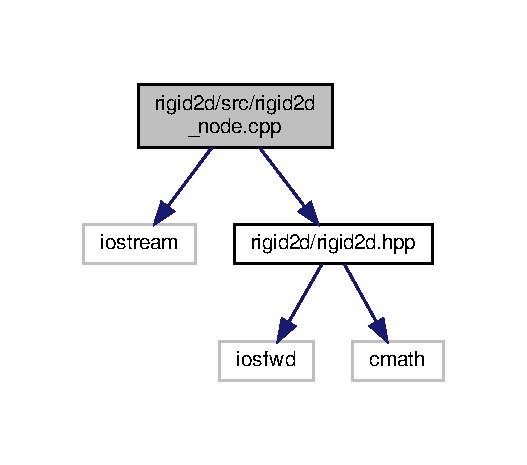
\includegraphics[width=253pt]{dd/d3c/rigid2d__node_8cpp__incl}
\end{center}
\end{figure}
\subsection*{Functions}
\begin{DoxyCompactItemize}
\item 
\mbox{\Hypertarget{rigid2d__node_8cpp_a840291bc02cba5474a4cb46a9b9566fe}\label{rigid2d__node_8cpp_a840291bc02cba5474a4cb46a9b9566fe}} 
int {\bfseries main} (void)
\end{DoxyCompactItemize}


\subsection{Detailed Description}
Manipulates 2D Transforms, Vectors, and Twists to test the ridig2d files. 


\hypertarget{turtle__rect_8cpp}{}\section{tsim/src/turtle\+\_\+rect.cpp File Reference}
\label{turtle__rect_8cpp}\index{tsim/src/turtle\+\_\+rect.\+cpp@{tsim/src/turtle\+\_\+rect.\+cpp}}


This file contains the source code for the turtle\+\_\+rect node. It pulls in parameters set from the yaml file and uses feed forward control to drive the turtle in a rectangle. It also calculates the positional error over time.  


{\ttfamily \#include $<$ros/ros.\+h$>$}\newline
{\ttfamily \#include \char`\"{}std\+\_\+srvs/\+Empty.\+h\char`\"{}}\newline
{\ttfamily \#include \char`\"{}turtlesim/\+Set\+Pen.\+h\char`\"{}}\newline
{\ttfamily \#include \char`\"{}turtlesim/\+Teleport\+Absolute.\+h\char`\"{}}\newline
{\ttfamily \#include \char`\"{}turtlesim/\+Pose.\+h\char`\"{}}\newline
{\ttfamily \#include \char`\"{}geometry\+\_\+msgs/\+Twist.\+h\char`\"{}}\newline
{\ttfamily \#include \char`\"{}tsim/\+Pose\+Error.\+h\char`\"{}}\newline
{\ttfamily \#include \char`\"{}rigid2d/rigid2d.\+hpp\char`\"{}}\newline
Include dependency graph for turtle\+\_\+rect.\+cpp\+:
\nopagebreak
\begin{figure}[H]
\begin{center}
\leavevmode
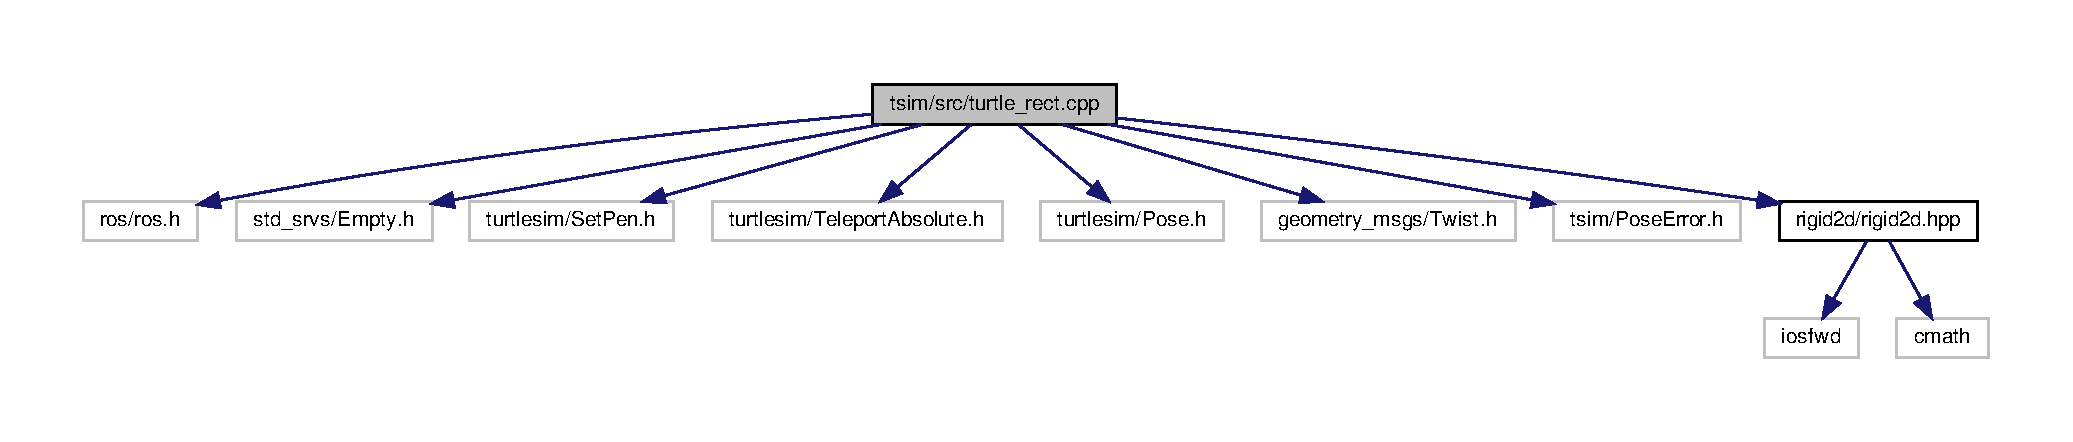
\includegraphics[width=350pt]{d7/df1/turtle__rect_8cpp__incl}
\end{center}
\end{figure}
\subsection*{Classes}
\begin{DoxyCompactItemize}
\item 
struct \hyperlink{structPoseVals}{Pose\+Vals}
\begin{DoxyCompactList}\small\item\em A struct to hold related positional values. \end{DoxyCompactList}\end{DoxyCompactItemize}
\subsection*{Functions}
\begin{DoxyCompactItemize}
\item 
\mbox{\Hypertarget{turtle__rect_8cpp_a10acaff3558ec865b3ddf7ac834a0efd}\label{turtle__rect_8cpp_a10acaff3558ec865b3ddf7ac834a0efd}} 
void \hyperlink{turtle__rect_8cpp_a10acaff3558ec865b3ddf7ac834a0efd}{teleport\+\_\+turtle} ()
\begin{DoxyCompactList}\small\item\em A helper function to teleport the turtle to the beginning of the trajectory. \end{DoxyCompactList}\item 
\mbox{\Hypertarget{turtle__rect_8cpp_a3bb8cd026aadeaeb2ab3eb9aa00eed6b}\label{turtle__rect_8cpp_a3bb8cd026aadeaeb2ab3eb9aa00eed6b}} 
void \hyperlink{turtle__rect_8cpp_a3bb8cd026aadeaeb2ab3eb9aa00eed6b}{calc\+\_\+error} ()
\begin{DoxyCompactList}\small\item\em Helper function to calculate the current positional error. \end{DoxyCompactList}\item 
\mbox{\Hypertarget{turtle__rect_8cpp_a4bb272c35c99026e08e491f264955c8f}\label{turtle__rect_8cpp_a4bb272c35c99026e08e491f264955c8f}} 
bool {\bfseries callback\+\_\+reset\+\_\+traj} (std\+\_\+srvs\+::\+Empty\+::\+Request \&, std\+\_\+srvs\+::\+Empty\+::\+Response \&)
\item 
\mbox{\Hypertarget{turtle__rect_8cpp_ae25546bb8a12b178c2644754e7875f1d}\label{turtle__rect_8cpp_ae25546bb8a12b178c2644754e7875f1d}} 
void \hyperlink{turtle__rect_8cpp_ae25546bb8a12b178c2644754e7875f1d}{callback\+\_\+pose} (const turtlesim\+::\+Pose \&msg)
\begin{DoxyCompactList}\small\item\em Callback function for the /turtle1/pose subscriber. \end{DoxyCompactList}\item 
\mbox{\Hypertarget{turtle__rect_8cpp_a3c04138a5bfe5d72780bb7e82a18e627}\label{turtle__rect_8cpp_a3c04138a5bfe5d72780bb7e82a18e627}} 
int \hyperlink{turtle__rect_8cpp_a3c04138a5bfe5d72780bb7e82a18e627}{main} (int argc, char $\ast$$\ast$argv)
\begin{DoxyCompactList}\small\item\em Main function to create the turtle\+\_\+rect node. \end{DoxyCompactList}\end{DoxyCompactItemize}


\subsection{Detailed Description}
This file contains the source code for the turtle\+\_\+rect node. It pulls in parameters set from the yaml file and uses feed forward control to drive the turtle in a rectangle. It also calculates the positional error over time. 

P\+A\+R\+A\+M\+E\+T\+E\+RS\+: g\+\_\+x (int) The x coordinate of the lower left corner of a rectangle g\+\_\+y (int) The y coordinate of the lower left corner of a rectangle width (int) The width of the rectangle height (int) The height of the rectangle trans\+\_\+vel (int) The translational velocity of the robot rot\+\_\+vel\+: (int) The rotational velocity of the robot frequency (int) The frequency of the control loop P\+U\+B\+L\+I\+S\+H\+ES\+: /pose\+\_\+error (tsim/\+Pose\+Error)\+: The positional error of the turtle at each cycle. /turtle1/cmd\+\_\+vel (geometry\+\_\+msgs/\+Twist)\+: The velcotiy command to control the turtle. S\+U\+B\+S\+C\+R\+I\+B\+ES\+: /turtle1/pose (turtlesim/\+Pose)\+: Retrieves the current pose of the turtle S\+E\+R\+V\+I\+C\+ES\+: /traj\+\_\+reset (std\+\_\+srvs/\+Empty)\+: resets the turtle to the beginning of the trajectory (lower left corner of the rectangle) 
\hypertarget{turtle__way_8cpp}{}\section{tsim/src/turtle\+\_\+way.cpp File Reference}
\label{turtle__way_8cpp}\index{tsim/src/turtle\+\_\+way.\+cpp@{tsim/src/turtle\+\_\+way.\+cpp}}


This file contains the source code for the turtle\+\_\+way node. It reads in a list of waypoints and sends commands to turtlesim to follow that path.  


{\ttfamily \#include $<$ros/ros.\+h$>$}\newline
{\ttfamily \#include \char`\"{}std\+\_\+srvs/\+Empty.\+h\char`\"{}}\newline
{\ttfamily \#include \char`\"{}turtlesim/\+Set\+Pen.\+h\char`\"{}}\newline
{\ttfamily \#include \char`\"{}turtlesim/\+Teleport\+Absolute.\+h\char`\"{}}\newline
{\ttfamily \#include \char`\"{}turtlesim/\+Pose.\+h\char`\"{}}\newline
{\ttfamily \#include \char`\"{}geometry\+\_\+msgs/\+Twist.\+h\char`\"{}}\newline
{\ttfamily \#include \char`\"{}tsim/\+Pose\+Error.\+h\char`\"{}}\newline
{\ttfamily \#include \char`\"{}rigid2d/rigid2d.\+hpp\char`\"{}}\newline
{\ttfamily \#include \char`\"{}rigid2d/diff\+\_\+drive.\+hpp\char`\"{}}\newline
{\ttfamily \#include \char`\"{}rigid2d/waypoints.\+hpp\char`\"{}}\newline
Include dependency graph for turtle\+\_\+way.\+cpp\+:\nopagebreak
\begin{figure}[H]
\begin{center}
\leavevmode
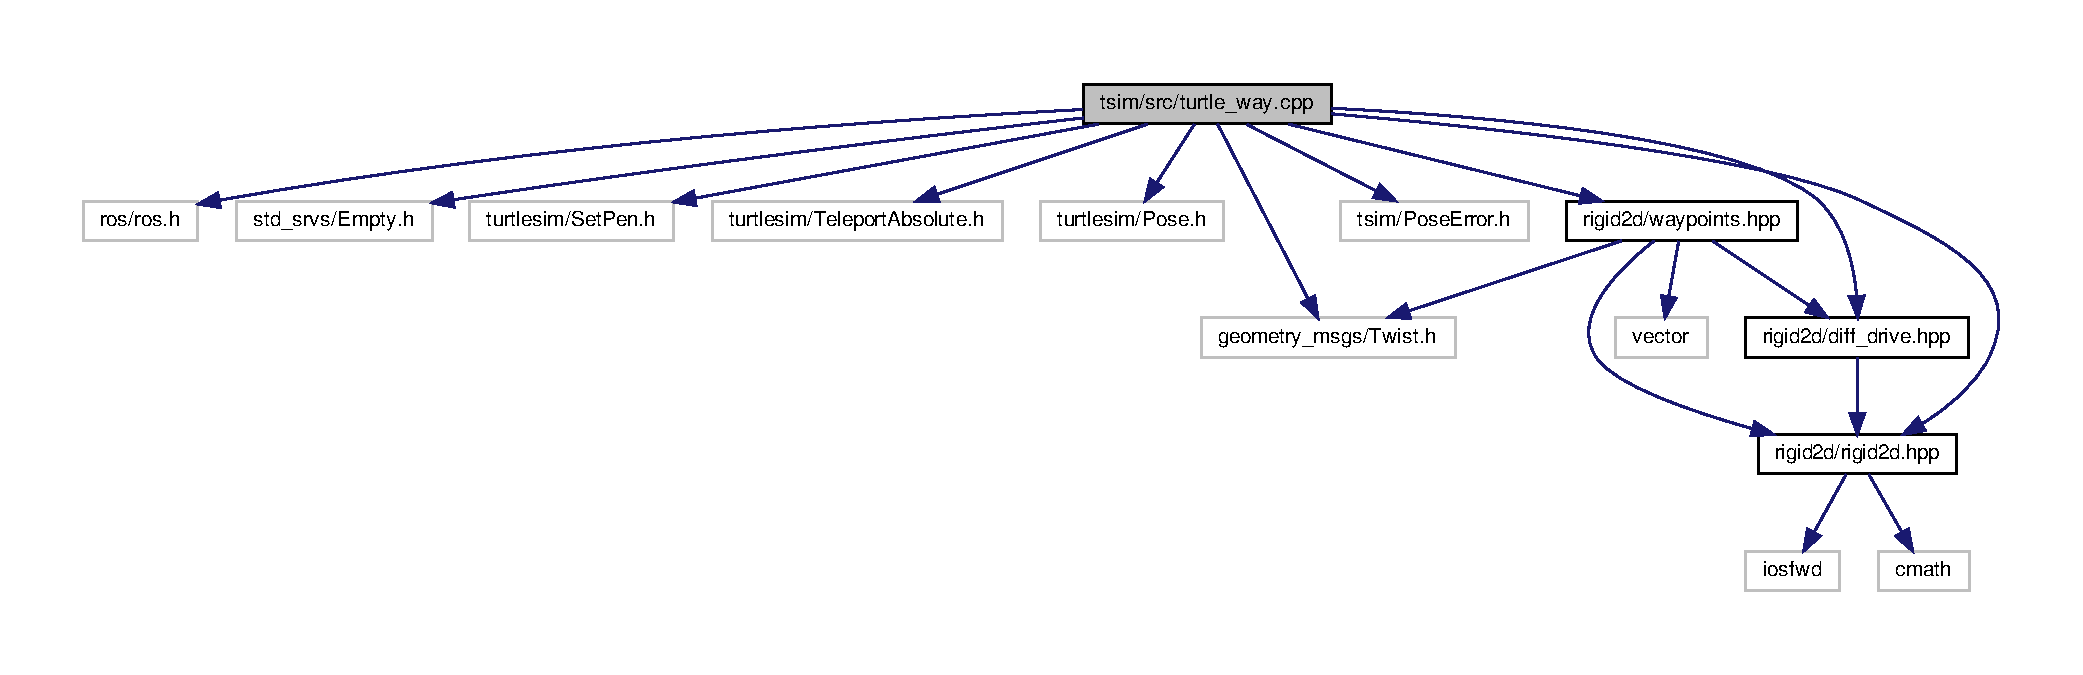
\includegraphics[width=350pt]{dd/dab/turtle__way_8cpp__incl}
\end{center}
\end{figure}
\subsection*{Functions}
\begin{DoxyCompactItemize}
\item 
\mbox{\Hypertarget{turtle__way_8cpp_aedd77161b6e4a108a487d13b225a51f3}\label{turtle__way_8cpp_aedd77161b6e4a108a487d13b225a51f3}} 
void \hyperlink{turtle__way_8cpp_aedd77161b6e4a108a487d13b225a51f3}{teleport\+\_\+turtle} (\hyperlink{structrigid2d_1_1Pose2D}{rigid2d\+::\+Pose2D} tele)
\begin{DoxyCompactList}\small\item\em A helper function to teleport the turtle to the beginning of the trajectory. \end{DoxyCompactList}\item 
\mbox{\Hypertarget{turtle__way_8cpp_a3bb8cd026aadeaeb2ab3eb9aa00eed6b}\label{turtle__way_8cpp_a3bb8cd026aadeaeb2ab3eb9aa00eed6b}} 
void \hyperlink{turtle__way_8cpp_a3bb8cd026aadeaeb2ab3eb9aa00eed6b}{calc\+\_\+error} ()
\begin{DoxyCompactList}\small\item\em Helper function to calculate the current positional error. \end{DoxyCompactList}\item 
\mbox{\Hypertarget{turtle__way_8cpp_ae25546bb8a12b178c2644754e7875f1d}\label{turtle__way_8cpp_ae25546bb8a12b178c2644754e7875f1d}} 
void \hyperlink{turtle__way_8cpp_ae25546bb8a12b178c2644754e7875f1d}{callback\+\_\+pose} (const turtlesim\+::\+Pose \&msg)
\begin{DoxyCompactList}\small\item\em Callback function for the /turtle1/pose subscriber. \end{DoxyCompactList}\item 
\mbox{\Hypertarget{turtle__way_8cpp_a3c04138a5bfe5d72780bb7e82a18e627}\label{turtle__way_8cpp_a3c04138a5bfe5d72780bb7e82a18e627}} 
int \hyperlink{turtle__way_8cpp_a3c04138a5bfe5d72780bb7e82a18e627}{main} (int argc, char $\ast$$\ast$argv)
\begin{DoxyCompactList}\small\item\em Main function to create the turtle\+\_\+way node. \end{DoxyCompactList}\end{DoxyCompactItemize}


\subsection{Detailed Description}
This file contains the source code for the turtle\+\_\+way node. It reads in a list of waypoints and sends commands to turtlesim to follow that path. 

P\+A\+R\+A\+M\+E\+T\+E\+RS\+: waypoint\+\_\+x\+: (int) A list of the x coordinates for a series of waypoints waypoint\+\_\+y\+: (int) A list of the y coordinates for a series of waypoints trans\+\_\+vel\+: (int) The translational velocity of the robot rot\+\_\+vel\+: (int) The rotational velocity of the robot frequency\+: (int) The frequency of the control loop wheel\+\_\+radius\+: (double) The radius of the wheels wheel\+\_\+base\+: (double) The distance between two wheels P\+U\+B\+L\+I\+S\+H\+ES\+: /pose\+\_\+error (tsim/\+Pose\+Error)\+: The positional error of the turtle at each cycle. /turtle1/cmd\+\_\+vel (geometry\+\_\+msgs/\+Twist)\+: The velcotiy command to control the turtle. S\+U\+B\+S\+C\+R\+I\+B\+ES\+: /turtle1/pose (turtlesim/\+Pose)\+: Retrieves the current pose of the turtle 
%--- End generated contents ---

% Index
\backmatter
\newpage
\phantomsection
\clearemptydoublepage
\addcontentsline{toc}{chapter}{Index}
\printindex

\end{document}
